% NYU PhD thesis format. Created by Jose Koiller 2007--2008.
% Adapted by Chen Wang 2016 July 27th
 
\documentclass[12pt,letterpaper]{report}
%% \usepackage[draft]{graphicx}

%% Replace the title, name, advisor name, graduation date and
%% dedication below with your own. Graduation months must be January,
%% May or September.
\newcommand{\thesistitle}{Closing the Loop: Holographic Feedback
for Soft-Matter Processes}
\newcommand{\thesisauthor}{Mark D. Hannel}
\newcommand{\thesisadvisor}{David G. Grier}
\newcommand{\graddate}{September, 2018}
\usepackage{fancyhdr}
\usepackage{graphicx}
\graphicspath{{./Figures/}}

%% This inputs your auxiliary file with \usepackage's and \newcommand's:
%% It is assumed that that file is called "definitions.tex".
%%%
%% Add your own definitions
%Packages to use
%%%%%%%%%%%%%%%%%%%%%%%%%%%%%%%%%%%%%%%%%%%%%%%%%%%%%%%%

\usepackage[nottoc]{tocbibind}
\usepackage[toc,page]{appendix}
% citations

\usepackage{cite}

\usepackage{geometry}               % See geometry.pdf to learn the
                                    % layout options. There are lots.
\usepackage{caption}
\captionsetup{font={stretch=1.5}}
\usepackage{color}
\usepackage{xcolor}
\usepackage{subcaption}  % Emma added it
\usepackage{amsmath,textcomp}
\usepackage{amssymb}
\usepackage{bm,upgreek}
\usepackage{enumerate}
\usepackage[utf8]{inputenc}

%\usepackage{fixmath}
%\usepackage[super,sort&compress,comma]{natbib}
\usepackage[numbers,square,sort&compress,comma]{natbib} 
%\usepackage[version=3]{mhchem}
%\usepackage{times,mathptmx}
%\usepackage{sectsty}
%\usepackage{balance}
%\usepackage{lastpage}
%\usepackage[format=plain,justification=raggedright,singlelinecheck=false,font=small,labelfont=bf,labelsep=space]{caption} 
%\usepackage{fancyhdr}
%\pagestyle{fancy}

%%%Jan Smreck packages
\usepackage{latexsym}
\usepackage{amsfonts}
\usepackage{hhline}
%%%%
\usepackage[separate-uncertainty=true,multi-part-units=single,per=slash,range-phrase=--,range-units=brackets,per-mode=symbol-or-fraction]{siunitx}
%\DeclareSIUnit{u}{\mu}
\usepackage{url}
\usepackage{indentfirst}
\usepackage{suffix}
\usepackage{tabularx}
\usepackage{booktabs}
\usepackage{parskip}
%% Controls spacing between lines (\doublespacing, \onehalfspacing,
%% etc.):
\usepackage{setspace}
\usepackage{hyperref}
\hypersetup{
	colorlinks=False,
        %hidelinks=True,
        %citecolor=blue,
        %urlcolor=black
        allcolors=black
}
%% ocgcolorlinks keeps colors for links when viewing via screen
%% but uses magic so that the links are black when printed.
\usepackage[ocgcolorlinks]{ocgx2} 
\usepackage[labelfont=bf]{caption}		%boldface caption labels

%\usepackage{xcolor,soul}
%	\sethlcolor{purple}
%\newcommand{\colorcomment}[1]{ {\color{white}\hl{  \bf #1 }}}
%modifying colors for links
%\colorlet{linkequation}{red}
%\usepackage[colorlinks=true,citecolor=blue,linkcolor=purple,urlcolor=black]{hyperref}
%\newcommand*{\SavedEqref}{}
%\let\SavedEqref\eqref
%\renewcommand*{\eqref}[1]{%
%	\begingroup
%	\hypersetup{
%		linkcolor=linkequation,
%		linkbordercolor=linkequation,
%	}%
%	\SavedEqref{#1}%
%	\endgroup
%}




%Define new commands
%%%%%%%%%%%%%%%%%%%%%%%%%%%%%%%%%%%%%%%%%%%%%%%%%%%%%%%%%%%%%%%%%%%%%


\renewcommand{\figurename}{\small{Fig.}~}
\renewcommand{\vec}[1]{\boldsymbol{#1}}
\newcommand{\oldvec}[1]{\vec{#1}}
%\renewcommand{\vec}[1]{\mathbf{#1}}
\newcommand{\uvec}[1]{\boldsymbol{\hat{#1}}}
\newcommand{\abs}[1]{\left\vert #1 \right\vert}
\newcommand{\imaginary}[1]{\Im\left\{ #1 \right\}}
\newcommand{\real}[1]{\Re\left\{ #1 \right\}}

\newcommand{\vecr}{\left(\vec{r}\right)}
\newcommand{\basisj}{\hat{e}_j}
\newcommand{\basis}{\left\{\basisj\right\}}
\newcommand\vectorpotential{\vec{A}\left(\vec{r},t\right)}
\WithSuffix\newcommand\vectorpotential*{\vec{A}^\ast\left(\vec{r},t\right)}
\newcommand{\electricfield}{\vec{E}\left(\vec{r},t\right)}
\WithSuffix\newcommand\electricfield*{\vec{E}^\ast\left(\vec{r},t\right)}
\newcommand{\magneticfield}{\vec{H}(\vec{r},t)}
\WithSuffix\newcommand\magneticfield*{\vec{H}^\ast\left(\vec{r},t\right)}
\newcommand{\amplitude}{u\vecr}
\newcommand{\ph}{\varphi}
\newcommand{\phj}{\ph_j}
\newcommand{\phase}{\ph\vecr}
\newcommand{\phasej}{\phj\vecr}
\newcommand{\pol}{\varepsilon}
\newcommand{\polj}{\pol_j}
\newcommand\polarization{\hat{\pol}\vecr}
\WithSuffix\newcommand\polarization*{\hat{\pol}^\ast\vecr}
\newcommand{\polarizationj}{\polj\vecr}
\WithSuffix\newcommand\polarizationj*{\polj^\ast\vecr}
\newcommand{\intensity}{I\vecr}
\newcommand{\action}{\mathcal{I}\vecr}
\newcommand{\momentum}{\vec{g}\vecr}
\newcommand{\spin}{\vec{s}}
\newcommand{\spindensity}{\spin\vecr}
\newcommand{\helicity}{\pmb{\sigma}\vecr}
\newcommand{\wavevector}{\vec{q}\vecr}
\newcommand{\wavenumber}{q\vecr}
\newcommand{\propagation}{\hat{q}\vecr}
%\newcommand{\orbitaldensity}{\vec{\ell}\vecr}
\newcommand{\orbitaldensity}{\pmb{\ell}\vecr}
\newcommand{\orbital}{\vec{\ell}\vecr}
\newcommand{\Lagr}{\mathcal{L}}

\newcommand{\mytilde}{\raise.17ex\hbox{$\scriptstyle\mathtt{\sim}$}}
\newcommand{\pos}{\left(\mathbf{r} \right)}
\newcommand{\bigN}[1]{\vec{N}_{nm}^{(#1)}(k\vec{r})}
\newcommand{\bigM}[1]{\vec{M}_{nm}^{(#1)}(k\vec{r})}

%Commands used by Jan Smreck for making list of appendices
\newcommand\listappendixname{List of Appendices}
\newcommand\appcaption[1]{%
  \addcontentsline{app}{section}{#1}}
\makeatletter
\newcommand\listofappendices{%
  \chapter*{\listappendixname}\@starttoc{app}}
\makeatother

%Commands hide a chapter from the table of contents
% from the following forum post:
% http://tex.stackexchange.com/questions/20543/excluding-chapters-from-toc-in-ams
\DeclareRobustCommand{\gobblefive}[5]{}
\newcommand*{\SkipTocEntry}{\addtocontents{toc}{\gobblefive}}

\makeatletter % Need for anything that contains an @ command 
\renewcommand{\maketitle} % Redefine maketitle to conserve space
{ \begingroup \vskip 10pt \begin{center} \large {\bf \@title}
	\vskip 10pt \large \@author \hskip 20pt \@date \end{center}
  \vskip 10pt \endgroup \setcounter{footnote}{0} }
\makeatother % End of region containing @ commands
\renewcommand{\labelenumi}{(\alph{enumi})} % Use letters for enumerate
% \DeclareMathOperator{\Sample}{Sample}
\let\vaccent=\v % rename builtin command \v{} to \vaccent{}
\renewcommand{\v}[1]{\ensuremath{\mathbf{#1}}} % for vectors
\newcommand{\gv}[1]{\ensuremath{\mbox{\boldmath$ #1 $}}} 
% for vectors of Greek letters
\newcommand{\uv}[1]{\ensuremath{\mathbf{\hat{#1}}}} % for unit vector
\newcommand{\avg}[1]{\left< #1 \right>} % for average

% For capital chapter references.
\let\orgautoref\autoref
\providecommand{\Autoref}[1]{\def\chapterautorefname{Chapter}\orgautoref{#1}}
\renewcommand{\autoref}[1]{\def\chapterautorefname{chapter}\orgautoref{#1}}


% Page setup
%%%%%%%%%%%%%%%%%%%%%%%%%%%%%%%%%%%%%%%%%%%%%%%%%%%%%%%%%%%%%%%%%%

%% The following makes chapters and sections, but not subsections,
%% appear in the TOC (table of contents). Increase to 2 or 3 to
%% make subsections or subsubsections appear, respectively. It seems
%% to be usual to use the "1" setting, however.
\setcounter{tocdepth}{2}

%% Sectional units up to subsubsections are numbered. To number
%% subsections, but not subsubsections, decrease this counter to 2.
\setcounter{secnumdepth}{3}

%% Page layout (customized to letter paper and NYU requirements):
\setlength{\parindent}{1.5cm}
\setlength{\oddsidemargin}{.35in}
\setlength{\textwidth}{5.8in}
\setlength{\topmargin}{.1in}
\setlength{\headheight}{0in}
\setlength{\headsep}{0in}
\setlength{\textheight}{8.3in}
\setlength{\footskip}{.5in}

%% Use the following commands, if desired, during production.
%% Comment them out for final version.
%\usepackage{layout} % defines the \layout command, see below
%\setlength{\hoffset}{-.75in} % creates a large right margin for notes and \showlabels


%% Use the line below for official NYU version, which requires
%% double line spacing. For all other uses, this is unnecessary,
%% so the line can be commented out.
\doublespacing % requires package setspace, invoked above

%% Each of the following lines defines the \com command, which produces
%% a comment (notes for yourself, for instance) in the output file.
%% Example:    \com{this will appear as a comment in the output}
%% Choose (uncomment) only one of the three forms:
%\newcommand{\com}[1]{[/// {#1} ///]}       % between [/// and ///].
\newcommand{\com}[1]{\marginpar{\tiny #1}} % as (tiny) margin notes
%\newcommand{\com}[1]{}                     % suppress all comments.


%% Cross-referencing utilities. Use one or the other--whichever you prefer--
%% but comment out both lines for final version.
%\usepackage{showlabels}
%\usepackage{showkeys}

%The Document
%%%%%%%%%%%%%%%%%%%%%%%%%%%%%%%%%%%%%%%%%%%%%%%%%%%%%%%%%%%%%%%%%%%%%
\begin{document}

%% Produces a test "layout" page, for "debugging" purposes only.
%% Comment out for final version.
%\layout % requires package layout (see above, on this same file)


    %%%%%%Preliminary pages
    %%%%%%%%%%%%%%%%%%%%%%%%%%%%%%%%%%%%%%%%%%%%%%%%%

    %% Sets page numbering to "roman style" i, ii, iii, iv, etc:
    \pagenumbering{roman}

    %%%%%% Title page %%%%%%
    \thispagestyle{empty}
\begin{center}
        
        {\large\textbf{\thesistitle}}
        
        \vspace{0.7in}
        by
        
        \vspace{0.7in}
        
        \text{\thesisauthor}
        
        \vspace{0.7in}
        
        \begin{doublespace}
           A dissertation submitted in partial fulfillment\\
           of the requirements for the degree of\\
           Doctor of Philosophy\\
           Department of Physics\\
           New York University\\
           \graddate
        \end{doublespace}
\end{center}
\vspace{.7in}
\noindent\makebox[\textwidth]{\hfill\makebox[2.5in]{\hrulefill}}\\
\makebox[\textwidth]{\hfill\makebox[2.5in]{\hfill\thesisadvisor\hfill}}

    \newpage
    
    %%%%%% Copyright %%%%%%
    %Copyright

\thispagestyle{empty}
\hbox{\ }

\vfill
\renewcommand{\baselinestretch}{1}
\small\normalsize

\vspace{-.65in}

\begin{center}
%\large
\normalsize{\copyright \hbox{ }
%Copyright by\\
\text{\thesisauthor}  %Type your name as it appears in University records
\\
\hspace{1in} \\
All Rights Reserved, 2018}
\end{center}

\vfill

    \doublespacing
    \newpage
    
    %%%%%% Blank page %%%%%%
    \thispagestyle{empty}
    \vspace*{0in}
    \newpage
    
    %%%%%% Copyright %%%%%%
    \chapter*{Dedication}
\addcontentsline{toc}{chapter}{Dedication}
\label{ch:list_of_appendices}
%\vspace*{\fill}
%\begin{center}  
%To my parents for starting this adventure and to all the lovely people, who at one time other, have joined me.
%\end{center}
\begin{quote}
  To my parents for starting this adventure and to all the lovely people, who at one time or another, have joined me.
\end{quote}
\vfill

    \newpage
    
    %%%%%% Acknowledgments %%%%%%
    \chapter*{Acknowledgments}
\addcontentsline{toc}{chapter}{Acknowledgments}
\label{ch:acknowledgments}

So long and thanks for all the fish!

    
    \newpage
    %\include{preface}
    %%%%%% Abstract %%%%%%
    \chapter*{Abstract}
\addcontentsline{toc}{chapter}{Abstract}
\label{ch:abstract}


\fancypagestyle{abstract_style}
{
\fancyhf{}
\lhead{{\bf Title: }\thesistitle\\
  {\bf Author: } \thesisauthor\\
  {\bf Advisor: } \thesisadvisor}
}

%\thispagestyle{abstract_style}

Colloidal systems exhibit a range of interesting behaviors that
underlie many fundamental processes and industrial applications.
Often these systems are comprised of
micrometer-sized constituents whose properties, namely their
size, refractive index, and three-dimensional position, can be measured
by holographic particle characterization (HPC).
The availability of this wealth of particle-resolved information
has inspired research activities around the world, and has rapidly
been adopted by industry.
Previous implementations of HPC have relied on \emph{ad hoc}
models and simplifying assumptions to extract information from
recorded holograms.
This thesis provides a firm foundation for the technique both by
advancing the theory of image formation in holographic microscopy
and also by reporting a suite of validation measurements
that establish the limits of precision and accuracy that can be
obtained from measurements based on holograms.

A particular focus of this work is to introduce and validate
the effective sphere model that extends the benefits of holographic
characterization to aspherical particles without incurring
an exorbitant cost in computational complexity.
In developing the effective sphere model, we furthermore 
introduce machine-learning implementations for fast and robust feature
detection and characterization.  These techniques enable us to
analyze dense and heterogeneous samples that ordinarily are
not amenable to optical characterization.
Finally, we apply our techniques to guide the design of colloidal
synthesis protocols, with a particular application to 
monodisperse spheres of 3-(trimethoxysilyl) propyl methacrylate
(TPM).

The effective sphere model proves to be an effective approach
to assess the properties of colloidal
systems compromised of aspherical particles such as rods,
aggregates, and dimpled spheres.
This line of inquiry addresses the question:
``To what extent does the Lorenz-Mie theory for light scattering
by spheres apply to aspherical and inhomogeneous colloidal particles?''
As a model system with a well-defined departure from sphericity,
we experimentally apply the effective sphere model to
characterizing dimpled spheres.
These studies demonstrate that standard holographic characterization
techniques yield a particle's radius to within \SI{1}{\percent} error
and its refractive index to within \SI{0.1}{\percent}
when the dimple comprises less than \SI{5}{\percent} of sphere's total volume.
Utilizing the discrete dipole
approximation, we simulate the scattering patterns of a myriad of
dimpled sphere geometries and find our experimental results are
typical for modest dimple sizes.

Heterogeneous samples pose a host of problems for automated
image analysis. Heuristics for detecting and localizing holographic
features typically employ a threshold which may overlook weaker
scatters or may identify several false positive in the vicinity of
overlapping features; dense, heterogeneous samples
particularly fall prey to these issues. To mitigate these constraints, we
develop two machine-learning implementations, namely convolutional
neural networks and cascade classifiers, to reduce the number of
false negative and false positive defections. 
Further characterization of a detected particle's properties require
sufficiently close initial parameter estimates so that the applied
fitting algorithm can converge to a global minimum.
 Given a heterogeneous sample
with disparate scatterer properties, a single \emph{a priori}
estimate may not suffice. We demonstrate that a class of machine-learning
algorithms known as support vector machines can be trained to
provide estimates of a scatterer's size, refractive index, and
position that are not only sufficient for bootstrapping subsequent
Lorenz-Mie analysis, but are accurate enough in themselves
for many end-use applications.

Methods for synthesizing colloidal spheres are often sensitive
to a multitude of protocol choices and environmental conditions. We
utilize HPC to investigate the synthesis of TPM spheres.
Specifically, we synthesize TPM spheres under a wide array of
conditions and apply holographic particle characterization to measure the
resulting distributions of particle size and refractive index.
The unique wealth of information provided by holographic characterization
enables us to assess directly how processing protocols influence
particles' final properties.


%HVM and pursuit of quantitative microscopy. Inherent assumptions
%and hang ups.
%This thesis validates and extends the domain of applicability for holographic characterization,
%and presents novel methods for analysis that enable new applications.

%Assumptions: Sphericity and vectorial nature of light propagation. Sphericity
% enables the effective sphere model.

%Analysis: Feature detection and localization. Enables analysis of denser flows, at a faster
%rate and with fewer false positives. Real time detection for automated trapping.
%ML for characterization. Automates and provides robust initial parameter estimation.
%Enables analysis of heterogeneous samples.

%Characterizing colloidal synthesis:  Utilizing HVM we will 


    %%%%%% Table of Contents %%%%%%
    {
      \hypersetup{linkcolor=black}
      \tableofcontents
    }
    \newpage

    %%%%%% List of Figures %%%%%%
    {
      \hypersetup{linkcolor=black}
      \listoffigures
    }
    \newpage

    %%%%%% List of Tables %%%%%%
    {
      \hypersetup{linkcolor=black}
      \listoftables
      }
    \newpage

    %%%%%% List of Appendices %%%%%%
    %If you have only one appedix comment this list of appendices out
    {
      \hypersetup{linkcolor=black}
      \listofappendices
    }
    \newpage
 
    %%%%%% Chapters %%%%%%
    %%%%%%%%%%%%%%%%%%%%%%%%%%%%%%%%%%%%%%%%%%%%%%%%%%%%%%%%
    \pagenumbering{arabic}
    
    \chapter{Introduction}
\label{ch:intro}

%    Move 1 establish your territory (say what the topic is about)
%    Move 2 establish a niche (show why there needs to be further research on your topic)
%    Move 3 introduce the current research (make hypotheses; state the research questions)


%    state the general topic and give some background
%    provide a review of the literature related to the topic
%    define the terms and scope of the topic
%    outline the current situation
%    evaluate the current situation (advantages/ disadvantages) and identify the gap
%    identify the importance of the proposed research
%    state the research problem/ questions
%    state the research aims and/or research objectives
%    state the hypotheses
%    outline the order of information in the thesis
%    outline the methodology

% https://www.scribbr.com/theses-examples/examples-dissertation-phd-theses/

% Soft matters ties to optical microscopy.
% Why advances in optical microscopy are necessary/fruitful.
% The advance of quantitative microscopy and HVM
% Outline of thesis in a narrative format.

% fluorescent labeling, super-resolution microscopy, digital microscopy
% provide increased localization.
% While ray optics paired with expensive optics leads researchers to
% interpret each microscopic image as a 1-to-1 depiction of life in the
% sample, the reality is much more complicated. Diffraction, real
% optics, focus.. images are complicated.
% Reseachers who want access to the deluge of quantitative
% information able via microscopy have 



\section{The pursuit of quantitative microscopy}

Microscopy has revolutionized the physical sciences by producing
detailed images of features that are invisible to the naked eye.
Optics manufacturing has 
Modern bright-field microscopes image samples up to the
Abbe diffraction limit \cite{abbe1873}
and several super-resolution techniques now exist for
circumventing this historic limit.
Many methods for extracting
quantitative information from microscopic images rely
on interpreting regions of contrast as features and
then 

Here we describe holographic particle characterization,
a quantitative microscopy technique, for extracting
the three-dimensional position, size, and refractive index of
colloidal scatterers. By 

\section{Organization}

% FIXME: Make Chapter part of the href.
Chapter \ref{ch:hvm} provides an extensive theoretical and practical
introduction to holographic particle characterization. The primary
experimental setup for all subsequent experiments is introduced.

In \autoref{ch:debye} we model the optical train to establish the
physical limits of HPC set by the imaging apparatus. The scattered
field and incident field are evaluated at several planes along the
optical train. The refraction of rays through optical element
may impart a phase shift, a polarization rotation and a scaling
of complex magnitude. We determine that a scalar theory
approximation successful accounts for the images arriving in the
focal plane for the range of scatterers we are interested in.

Chapter \ref{ch:dimpled} presents a series of experimental and
simulated studies to determine the effective of Lorenz-Mie
microscopy in characterizing slight aspherical particles.
Specifically, we synthesize three types of colloidal particles:
spheres, spheres will small dimples and spheres with large dimples.
The work of this chapters validates the use of the Lorenz-Mie theory
for analyzing spheres which have small geometrical deviations from
ideal sphericity. Additionally, our work determines that the Lorenz-Mie
theory acts as an effective sphere model for particles with
pronounced deviations from a spherical geometry and provides
accurate information on the scatterer.

The first step in holographic particle characterization
requires detecting and localizing holographic features in experimental
images. Heuristic algorithms perform admirably for isolated, homogeneous
features; after tuning the necessary empirical parameters, they achieve
sub-pixel localization while incurring few false positives. However their
performance deteriorates when presented overlapping features or even
heterogenous holographic features (axial range, size and refractive index).

We present in \autoref{ch:cascade} two machine-learning algorithms for
detecting and localizing holographic features: a convolution
neural network (CNN) and a cascade classifier. Direct comparison with the
heuristic algorithm over a range of experimental and synthetic images
shows promising results. The CNN demonstrates robust feature detection
for overlapping holograms or even highly heterogeneous holographic features
in the same image. The cascade classifier's localization precision
offers is a ten times worse than the CNN, but is also ten times faster than
the CNN. In fact the cascade classifier is fast enough for real-time
applications such as high-speed targeting in holographic optical
trapping systems.

After detecting a holographic feature, an initial estimate of the
scatter's size, refractive index, and three-dimensional position
is necessary for the subsequent fit to the Lorenz-Mie theory.
For homogeneous samples of a single particle type, the fitting procedure
can be bootstrapped with outside information. For heterogeneous samples
with disparate sizes or refractive indices, the fitting procedure
will likely lock onto local minima and return erroneous results for
the size and refractive index. holographic features to the Lorenz-Mie theory requires
In \autoref{ch:svr} we demonstrate the use of a support vector machine for
estimating the size and refractive index of scatterers from snapshots
of holographic features. Our implementation has several steps. Our fitting
algorithm usually fits the intensity pattern from \SI{40000}{} pixels;
We reduce the dimensionality of this problem by analyzing the radial
profile of the image made by taking an average over angles. In addition
we produce a SVM for the three properties we need to bootstrap:
size, refractive index, and height above the focal plane. We demonstrate these
support vector machines can resolve heterogeneous samples with four greatly
differing particle properties.

In the previous chapters we have worked towards validating and extending
the domain of applicability of holographic particle characterization.
In \autoref{ch:synthesis} we close with a demonstration of its use for
analyzing the synthesis of \num{3}-methacryloxypropyltrimethoxysilane (TPM) colloidal
spheres. The synthesis is principally a two-step procedure: a emulsion of monodisperse,
micrometer sized TPM droplets is prepared and then polymerized.
A number of experimental parameters and conditions can however affect
the resulting size of the polymerized spheres. In this chapter we use
holographic particle characterization to analyze liquid droplets and
solid TPM spheres. By synthesizing particles under a number of
differing protocols, we isolate a number of experimental conditions
that affect particle size.

    \newpage

    \chapter{Holographic Video Microscopy}
\label{ch:hvm}

\newcommand{\einc}{\vec{E}_{\text{inc}}}
\newcommand{\escat}{\vec{E}_{\text{s}}}
\newcommand{\eadd}{\vec{E}_{\text{add}}}

\section{Overview}

Holographic video microscopy (HVM) uses coherent
illumination to measure properties of micrometer-sized particles,
primarily their size, refractive index, and three-dimensional position.
Coherent imaging preserves the phase information that is averaged-away
in conventional incoherent image. The physical properties of individual
scatterers are encoded in this phase information and can be extracted by fitting
the resulting intensity patterns to an appropriate light scattering theory.
For non-absorbing dielectric spheres between $\num{1}$-$\SI{10}{\um}$,
this technique yields nanometer-scale precision for the three-dimensional
position and radius, and part-per-thousand precision for the refractive
index\cite{krishnatreya14}.

In this chapter, we acquaint the reader with our primary experimental
HVM setup and in so doing outline the salient physical processes underlying
the technique. We then describe the Lorenz-Mie theory of light
scattering that provides the basis for our analytical technique,
discuss our implementation of image analysis, and 
conclude with a number of applications of holographic video
microscopy.

\section{Experimental Setup}
\label{ch:hvm:sec:hvm}

Fig.~\ref{fig:hvm_setup} presents our custom-built in-line holographic
microscope. Our setup illuminates the sample plane with a blue
($\SI{447}{nm}$ vacuum wavelength), linearly polarized laser beam
(Coherent Cube) to within \SI{1}{\degree} of the horizontal
axis of the camera. 
The beam's $\SI{25}{\mW}$ of power is spread over
the $\SI{3}{\mm}$ beam diameter, producing an average irradiance
of $\SI{0.88}{\mW / \mm^2}$. Before illuminating the sample, the beam
passes through a quarter-wave plate and a polarizing beam splitter
(ThorLabs CCM1-PBS251) to direct the beam's linear polarization, to
enable beam attenuation and to provide an optical pathway for
optional bright-field illumination.


\begin{figure}
  \centering
  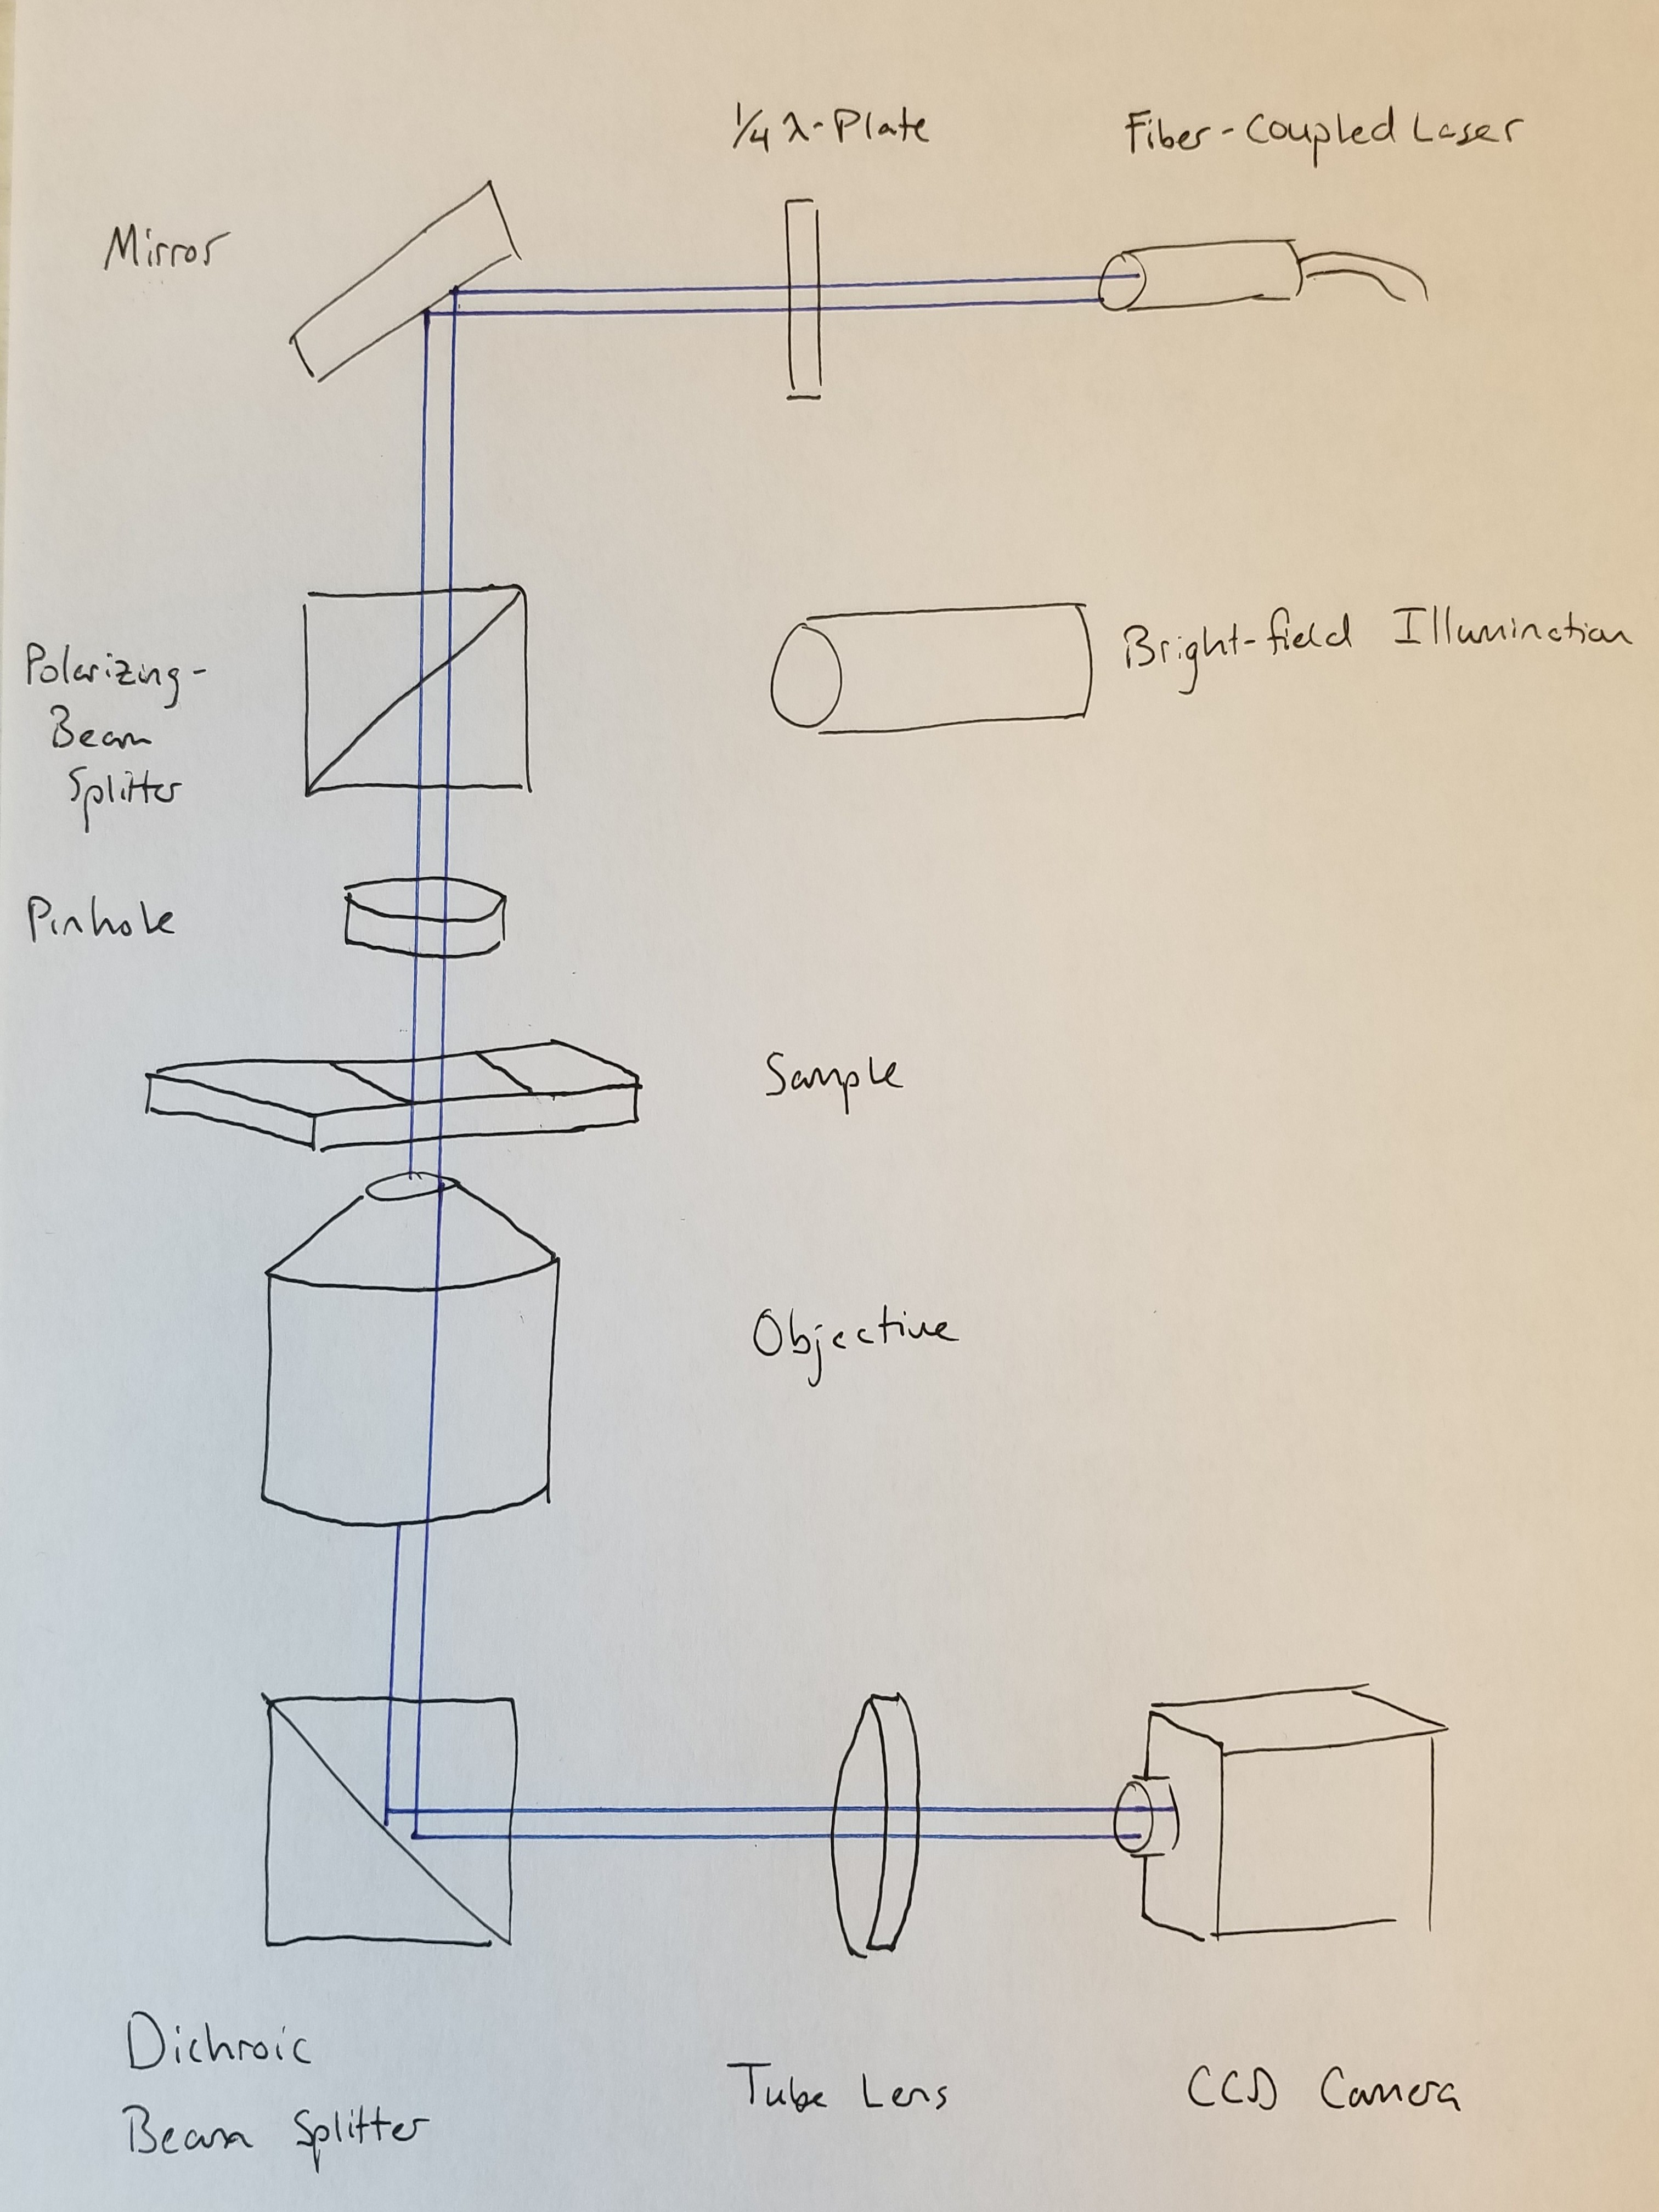
\includegraphics[width=\textwidth]{hvm_setup}
  \caption{A schematic of an inline holographic video microscope.}
  \label{fig:hvm_setup}
\end{figure}


The coherent illumination and light scattered by the sample are collected by a
standard microscope objective (Nikon Plan Apo, $\num{100}\times$,
numerical aperture $\num{1.45}$, oil immersion) and then focused
by a $\SI{200}{\mm}$ tube lens onto a grayscale digital camera
(NEC TI-324AII). The digital camera digitizes the resulting intensity
pattern to $8$-bits per pixel at $\SI{29.97}{frames / \sec}$ and relays the
resulting array of data to either a DVR (Pioneer 520HS) to record
on a DVD or directly to the hard disk of a personal computer.
Each pixel in the $\si{640\times 480}$ array of pixels has a width of
$\SI{13.5}{\um}$. After $100\times$ magnification, a pixel in the
image has an effective size of $\SI{0.135}{\um}$.

Each recorded image documents the interference between the incident
electric field and the resulting scattered waves. By fitting
to a theory of light scattering, we will measure the physical
properties of the scatterers contributing to the scattered field
at the focal plane of the objective.

% Description of trapping?


  % BLURB connecting HVM to DHM
%Holographic video microscopy is one of several
%digital holographic microscopy (DHM) techniques.
%DHM differs from traditional bright-field microscopy
%by preserving, collecting, and making quantitative use of phase
%information. In most variants of DHM, each recorded
%wavefront can be numerically reconstructed, or rather
%{\it un}-propagated, all the way back to a scattering event
%to produce an image of the scatterer. By reconstructing
%several planes around the scatterer, each hologram
%can provide insight into the topography of each scatter
%in the field of view.

%Holographic video microscopy differs from DHM by analytically
%fitting the scatter's properties to the resulting

\begin{figure}
  \centering
  \includegraphics[width=\textwidth]{hvm_image_formation}
  \caption{A time series depicting the image formation process. (a) the incident
    electric field propagates in the $+\hat{z}$ direction. (b) the
    incident field passes through a spherical scatterer causing a
    spherically expanding scattered wave in response. (c) the incident
    field and the scattered field combine at the focal plane to produce
    an image.}
  \label{fig:image_formation}
\end{figure}


\subsection{Image formation}
\label{ch:hvm:sec:hvm:ssec:overview}

The image formation process at the focal plane of the objective
is depicted in Fig.~\ref{fig:image_formation}. Fig.~\ref{fig:image_formation}(a)
shows the coherent illumination, or incident field $\einc (\vec{r})$, propagating in the $+\hat{z}$ direction
through the sample and toward the focal plane of the objective. We model the incident field
as a plane wave polarized in the $\hat{x}$ direction, 
\begin{equation}
  \label{eq:incidentfield}
  \einc(\vec{r}) = E_0\,  e^{i \varphi_0(\vec{r})} \, e^{i kz} \, \hat{x},
\end{equation}
with magnitude $E_0$, phase profile $\varphi_0(\vec{r})$, and wavenumber
$k = 2\pi n_m/\lambda$. All of the waves considered here
propagate with a time dependence of $e^{-i \omega t}$. Measurements of
the light's intensity are time averaged over the duration of the camera's exposure
period of at least $\SI{10}{\us}$. As we will be imaging with $\SI{447}{nm}$ blue
light ($\omega \approx \SI{670}{THz}$), our time average will include
nearly \num{7} billion full cycles. We will therefore safely neglect the time
dependence in all of our waves.


\begin{figure}
  \centering
  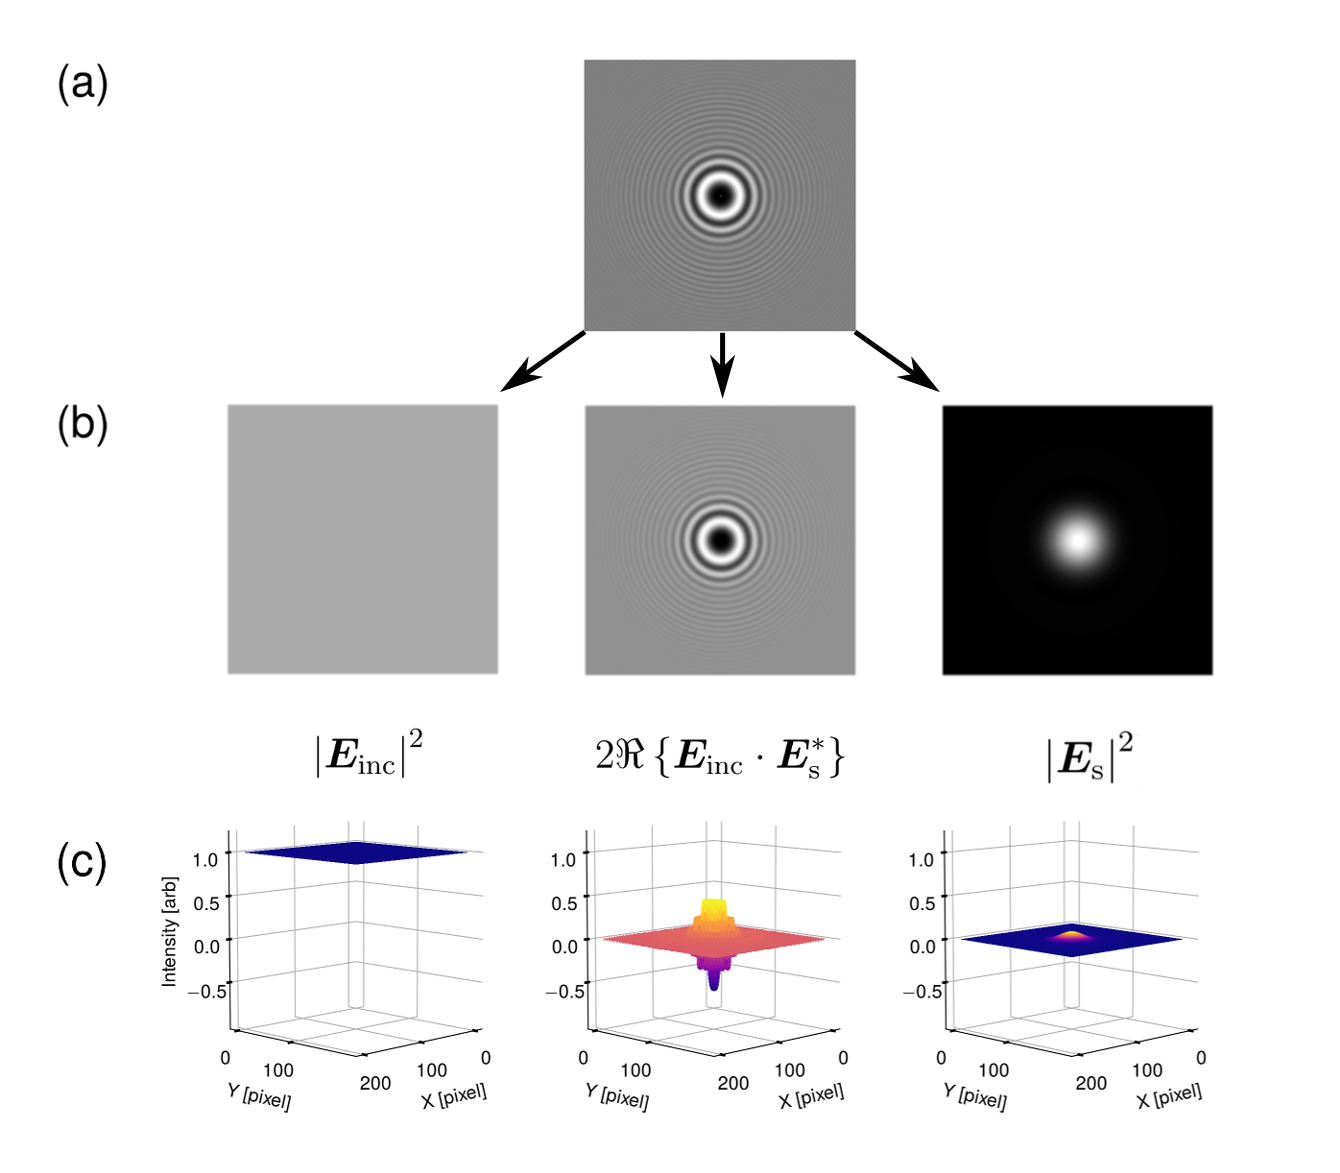
\includegraphics[width=\textwidth]{hvm_three_contributions}
  \caption{Depicting the three contributions to a holographic image. (a) the
    resulting intensity from a micrometer-sized scatterer above the focal plane.
    (b) the three contributions shown separately. (c) the magnitude of intensity
  for each term normalized by the intensity of the incident field.}
  \label{fig:three_contributions}
\end{figure}

As the incident illumination propagates freely through the sample, scatterers
whose refractive index differs from the medium's will emit a diverging scattered wave,
$\escat(\vec{r})$, in response. Fig.~\ref{fig:image_formation}(b) depicts the incident
field and resulting scattered field propagating toward the focal plane.
For the scatterers of interest in this study, the scattered field is dominated by
forward scattering and the scatterer absorbs a negligible proportion of the
incident wave.

The incident field and scattered field continue propagating and eventually pass through
the focal plane, as depicted in Fig.~\ref{fig:image_formation}. The intensity of the image
formed in the focal plane can be described as
\newcommand{\preint}{\frac{n_mc\epsilon_0}{2}}
\begin{align}
  I(\vec{r}) &= \preint\abs{\einc + \escat}^2\\
    &= \preint\left ( \abs{\einc}^2 + \einc\cdot\escat^* + \einc^*\cdot\escat + \abs{\escat}^2 \right ) \\
    &= \preint\left (\abs{\einc}^2 + 2\Re\left \{\einc\cdot\escat^*\right \} + \abs{\escat}^2 \right ) \label{eq:image_formation}
\end{align}
where $n_m$ is the refractive index of the medium, $c$ is the speed of light in a vacuum,
$\epsilon_0$ is the vacuum permittivity. We assumed that the medium is non-magnetic
($\mu_r=1$).

The relative contributions of the terms in Eq.~\eqref{eq:image_formation}
are depicted in Fig.~\ref{fig:three_contributions} for a $\SI{1.0}{\um}$ polystyrene
sphere ($n = 1.59$) a distance of $\SI{12}{\um}$ above an imaging plane with pixel
size $\SI{0.135}{\um}$.
The first term, $\abs{\einc}^2$ is constant over the field of view and
incorporates no phase information. The third term,
$\abs{\escat(\vec{r})}^2$, is also real-valued but is not constant over the field of view.
The second term, $2\Re\left \{\einc\cdot\escat^*(\vec{r})\right \}$, contributes the
spatially-varying interference pattern from the relative phase of the incident
beam and the scattered wave and the intensity variations of the scattered wave.
% Discussion of DC terms? Does DC Stand for duty cycle?
% Pull out E_0?
% Discuss relative sizes of terms.

\subsection{Scattering}
\label{ch:hvm:sec:hvm:ssec:scattering}

It is a general principle of scattering in linear homogeneous media
that the magnitude of the scattered wave be proportional to the
magnitude of the illuminating wave. We therefore model the scattered
field as
\begin{equation}
  \label{eq:gen_scattered}
  \escat(\vec{r}) = E_0(\vec{r}_p)\, \vec{f}_s \left ( k \left ( \vec{r} - \vec{r}_p \right ) \right ) ,
\end{equation}
where $E_0(\vec{r}_p)$ is the amplitude of the wave illuminating the scatterer at $\vec{r}_p$,
and $\vec{f}_s(\vec{r})$ describes how the particle $s$ scatters $\hat{x}$-polarized light.
Note that nature of $\vec{f}_s(\vec{r})$ depends inherently on the shape and composition
of the scatterer.

When the scattered field is adequately described by \eqref{eq:gen_scattered}, the
image in the focal plane linearly scales with the incident field intensity $\abs{\einc}^2$,
\begin{equation}
  \label{eq:gen_norm}
  I(\vec{r}) = \abs{\einc}^2\abs{\uvec{x} + \vec{f}_s(k(\vec{r}-\vec{r}_p))}^2
\end{equation}


With the exception of \autoref{ch:dimpled}, our study will focus exclusively on
spherical scatterers. The Lorenz-Mie theory offers an exact solution for $\vec{f}_s(\vec{r})$
in the case of a spherical scatterer illuminated with $\hat{x}$-polarized light.
We will provide a brief overview of the Lorenz-Mie theory to build intuition
for the scattered wave's dependence on the spherical scatter's properties; an exhaustive
account is provided in reference \cite{bohren83}.



\subsubsection{Lorenz-Mie Theory}
\label{ch:hvm:sec:hvm:ssec:scattering:sssec:lm_theory}

\begin{figure}
  \centering
  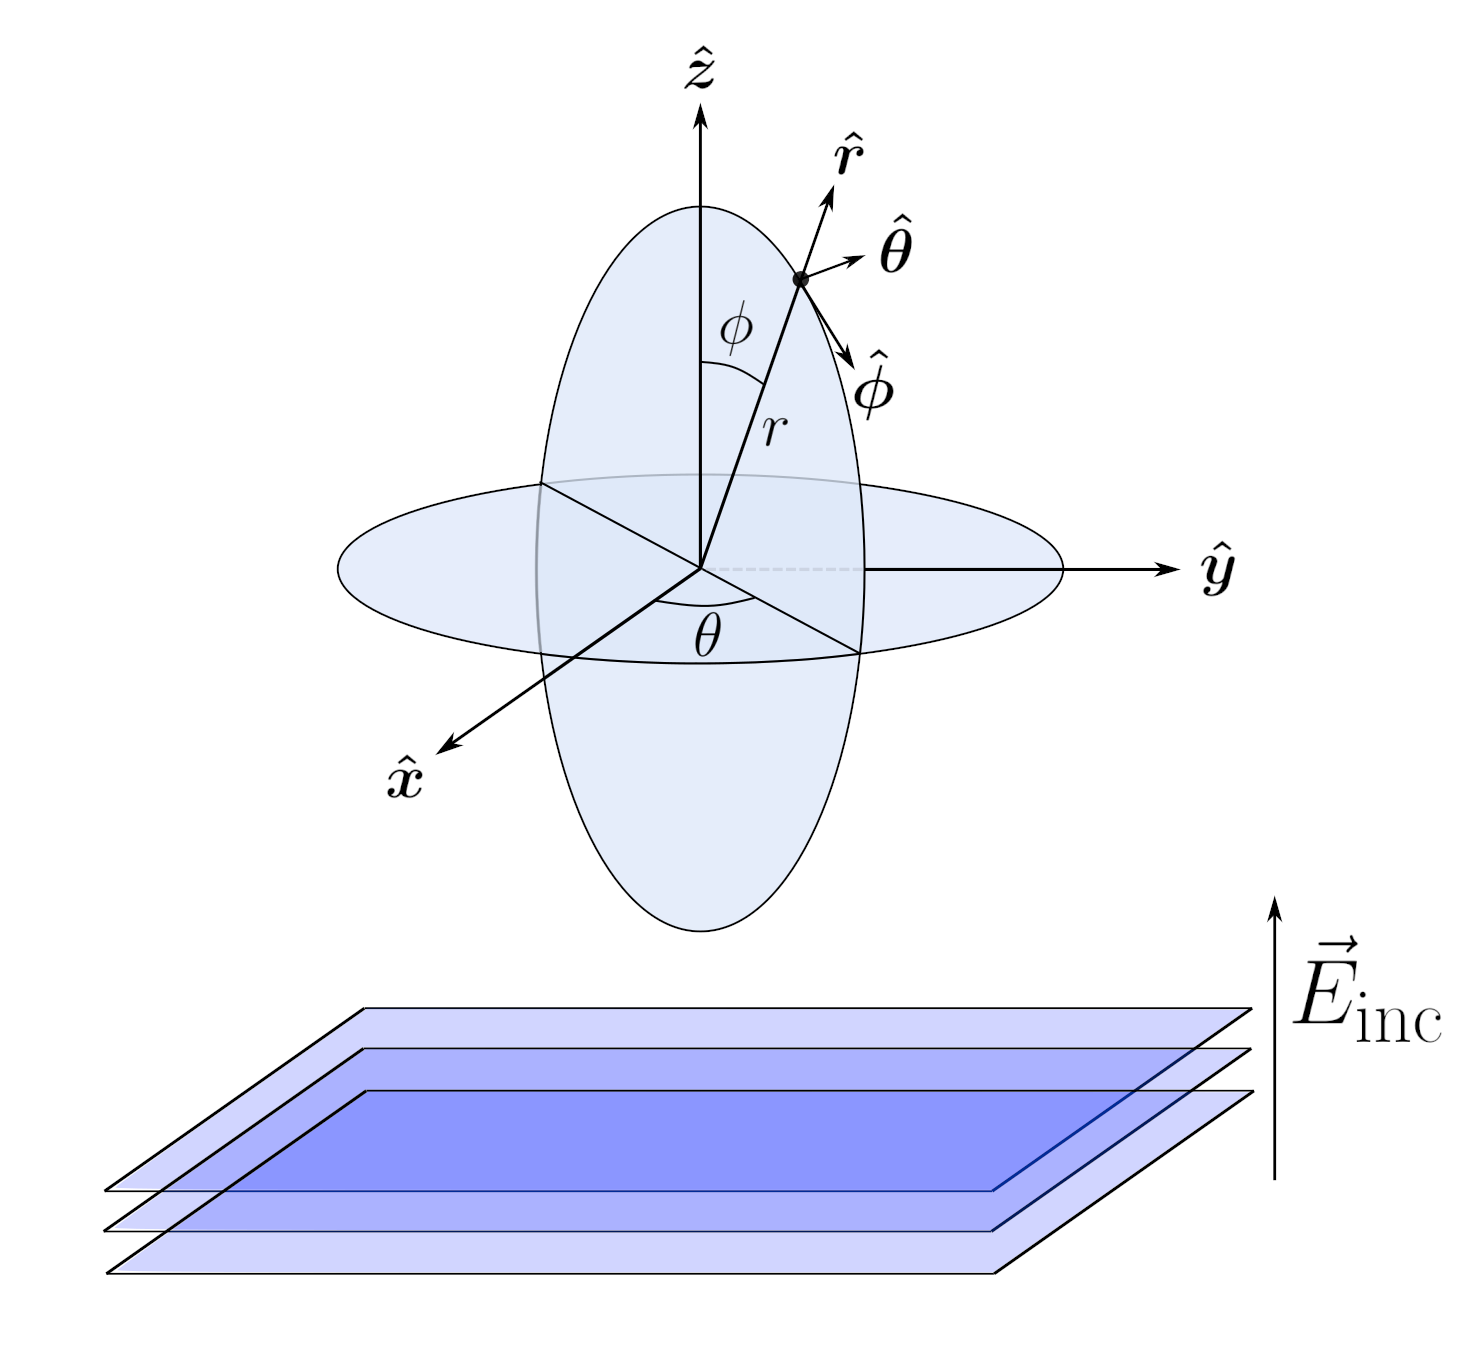
\includegraphics[width=0.5\columnwidth]{hvm_spherical_coords}
  \caption{Spherical coordinates for describing the Lorenz-Mie theory.
    The origin of the coordinate system rests at the center of the
    spherical scatterer. For viewing ease, the positive $\uvec{z}$ direction
  is depicted upwards, the opposite of Fig.~\ref{fig:image_formation}.}
  \label{fig:hvm_spherical_coords}
\end{figure}

We begin with a homogeneous, dielectric sphere of radius $a_p$ and refractive
index $n_p$ situated in a medium with refractive index $n_m$ at a position
$r_p$. We define a spherical coordinate system whose origin coincides with
the sphere as depicted in Fig.~\ref{fig:hvm_spherical_coords}
The incident beam is modeled as a plane wave of the form
\eqref{eq:incidentfield} which propagates toward
the scatterer from the $-\hat{z}$ direction. The scattering event
leads to three fields, namely the incident field, an external scattered
field, and an internal scattered field, all of which must match boundary conditions
at the surface of the sphere.  Based on the work of Kla\u{c}ka \emph{et al}~\cite{klacka07},
we conclude that the electrostatic
potential at the surface of a micrometer-scale sphere would have to be implausibly high
($\SI{E8}{V}$) before surface charge or current would appreciably affect the scattering
of visible light and therefore a recorded image. Therefore,
we adopt the usual assumption of a charge-free and current-free surface.

The internal and external fields in the vicinity of a sphere are most naturally
expressed as an expansion in vector spherical harmonics. Vector spherical harmonics
provide an orthonormal basis for the solutions to Maxwell's wave equations in free space.
The Lorenz-Mie solution amounts to expressing the incident plane wave as
a sum of vector spherical harmonics and matching the boundary conditions
at the surface of the spherical scatterer. After matching the boundary
conditions\cite{bohren83,mishchenko96}, the resulting external scattering function is
%The Lorenz-Mie theory
%constitutes an exact solution for a plane wave scattering off of a
%dielectric sphere in a homogeneous medium.

\begin{equation}
\label{eq:scatteredfield}
  \vec{f}_s(k \vec{r}) = \sum_{n=1}^\infty \, f_n \, \left(
    i a_n \, \vec{N}^{(3)}_{e1n}(k \vec{r}) - b_n \,
    \vec{M}^{(3)}_{o1n}(k \vec{r})
    \right),
\end{equation}
where $f_n=i^n (2n+1)/[n(n+1)]$, and $\vec{M}^{(3)}_{o1n}(k\vec{r})$ and 
$\vec{N}^{(3)}_{e1n}(k\vec{r})$ are the vector spherical harmonics,
\begin{equation}
    \vec{M}^{(3)}_{o1n}(k\vec{r}) = \frac{\cos\phi}{\sin\theta} \,
  P^1_n(\cos\theta) \, j_n(\rho) \, \uvec{\theta}
  - \sin\phi \, \frac{dP^1_n(\cos\theta)}{d\theta} \, j_n(\rho) \, \uvec{\phi},
\end{equation}
and
\begin{multline}
  \vec{N}^{(3)}_{e1n}(k\vec{r}) = n(n+1) \, \cos\phi
  \,P^1_n(\cos\theta) \, \frac{j_n(\rho)}{\rho} \, \uvec{r} \\
  + \cos\phi \, \frac{dP^1_n(\cos\theta)}{d\theta} \,
  \frac{1}{\rho} \frac{d}{d\rho}\left[ j_n(\rho)\right] \, \uvec{\theta} \\
  - \frac{\sin\phi}{\sin\theta} \, P^1_n(\cos\theta) \,
  \frac{1}{\rho}\frac{d}{d\rho}\left[\rho j_n(\rho)\right] \, \uvec{\phi}
\end{multline}
Here, $\rho = kr$ is the reduced radial coordinate,
$P^1_n(\cos\theta)$ is the associated Legendre polynomial of the
first kind, and $j_n(\rho)$ is the spherical Bessel function of the
first kind of order $n$.
The expansion coefficients $a_n$ and $b_n$ in Eq.~(\ref{eq:scatteredfield})
are given by \cite{bohren83}

\begin{equation}
  \label{eq:an}
  a_n = \frac{n_p^2 \, j_n(x_p) \left[x_m \, j_n(x_m)\right]^\prime -
    n_m^2 \, j_n(x_m) \left[x_p \, j_n(x_p)\right]^\prime}{
    n_p^2 \, j_n(x_p) \left[x_m \, h^{(1)}_n(x_m)\right]^\prime -
    n_m^2 \, h^{(1)}_n(x_m) \left[x_p \, j_n(x_p)\right]^\prime},
\end{equation}
and
\begin{equation}
\label{eq:bn}
  b_n = \frac{j_n(x_p) \left[x_m \, j_n(x_m)\right]^\prime -
    j_n(x_m) \left[x_p \, j_n(x_p)\right]^\prime}{
    j_n(x_p) \left[x_m \, h^{(1)}_n(x_m)\right]^\prime -
    h^{(1)}_n(x_m) \left[x_p \, j_n(x_p)\right]^\prime},
\end{equation}
%\begin{equation}
%  a_n = \frac{m^2 j_n(mka_p) \left[ka_p \, j_n(ka_p)\right]^\prime -
%    j_n(ka_p) \left[mka_p \, j_n(mka_p)\right]^\prime}{
%    m^2 j_n(mka_p) \left[ka_p \, h^{(1)}_n(ka_p)\right]^\prime -
%    h^{(1)}_n(ka_p) \left[mka_p \, j_n(mka_p)\right]^\prime},
%\end{equation}
%and
%\begin{equation}
%\label{eq:bn}
%  b_n = \frac{j_n(mka_p) \left[ka_p \, j_n(ka_p)\right]^\prime -
%    j_n(ka_p) \left[mka_p \, j_n(m ka_p)\right]^\prime}{
%    j_n(mka_p) \left[ka_p \, h^{(1)}_n(ka_p)\right]^\prime -
%    h^{(1)}_n(ka_p) \left[mka_p \, j_n(mka_p)\right]^\prime},
%\end{equation}
where $^\prime$ denotes the derivative of the function with respect
to the argument in parentheses and $x_m = \frac{2\pi n_m}{\lambda} a_p$
and $x_p = \frac{2\pi n_p}{\lambda} a_p$ are the reduced particle size according
to the medium and to the particle respectively. The infinite
sum in \eqref{eq:scatteredfield} can be safely truncated after
$x_m + 4x_m^{\frac{1}{2}} + 2$ terms\cite{wiscombe80}.

A few comments will at this point help to understand how \eqref{eq:gen_norm} through
\eqref{eq:bn} can be used to track and characterize colloidal particles.
The vector spherical harmonics do not depend on the scatterer's properties;
the scatterer's influence on the external scattered field is completely contained
in the coefficients.
The coefficients $a_n$ and $b_n$ converge to zero as $n_p$ approaches $n_m$ which
is the case for index-matched particles.
The condition for terminating the series in \eqref{eq:scatteredfield} depends only on refractive
index of the medium and the size of the particle in units of the wavelength. Given a medium
refractive index of $1.33$ and wavelength of $\SI{447}{\nm}$, the number of terms range from
approximately $50$ for a $\SI{1}{\um}$ sphere to $\num{240}$ for a $\SI{10}{\um}$ sphere.
% Should n_p = n_m.. these computations would be a waste!


\subsection{Image Analysis}

We analyze each of our recorded images to extract information about the particles
scattering light into the field of view.  Because the scattered wave's electric
field approximately decays as $r^{-1}$, each scatterer's influence on the
resulting image is confined to a sub-region of the image; we will
regard each of these regions of interest as holographic features.  Given an experimental
image, our task will be to isolate these holographic features and fit each
to the Lorenz-Mie theory.


\begin{figure}
  \centering
  \includegraphics[width=\textwidth]{hvm_image_analysis}
  \caption{Depicting the image analysis .}
  \label{fig:image_analysis}
\end{figure}


The entire image analysis procedure is depicted in Fig.~\ref{fig:image_analysis}.
Image normalization is a necessary pre-processing step; Normalizing
the image eliminates the incident beam's magnitude $\abs{\einc}^2$
as a fitting parameter, mitigates the contributions of additional
scatterers, and accounts for the digitization procedure of the camera.
We therefore fit to a normalized image $b(x,y)$ as
\begin{align}
  b(x,y) &= \frac{ I(x,y) - I_d(x,y)}{ I_{bg}(x,y) - I_d(x,y)} 
\end{align}
where $I(x,y)$ is the image recorded by the camera,
$I_{bg}(x,y) = \abs{\einc(\vec{r})}^2$ is the background intensity,
$I_d(x,y)$ is the dark count of the camera.
Fig.~\ref{fig:image_analysis}(a) demonstrates the effect of normalization.

The normalized image may or may not contain holographic features. If a feature
is detected,
our estimate of it's center will serve as an initial estimate
for the in-plane position of the associated scatterer.
Feature detection and feature localization are the first two steps in analyzing
normalized holograms. A common heuristic is to condense the
extended holographic features into localized blobs and then to use a standard
centroid finding algorithm\cite{crocker96} on the transformed image. In this way, the centers
of each blob will correspond to the center of a holographic feature. Fig.~\ref{fig:image_analysis}(b)
summarizes this heuristic algorithm. An in-depth study of this algorithm, as well
as machine-learning alternatives will be presented in \autoref{ch:cascade}.

We fit each localized holographic feature to the Lorenz-Mie theory
with the Levenberg-Marquardt algorithm, otherwise known as damped least-squares.
The Levenberg-Marquardt algorithm interpolates between gradient descent which is a damped
first order algorithm, 
and the Gauss-Newton algorithm which is a second order algorithm directed towards the nearest
minimum. As with many fitting algorithms, this method find a local
minimum which may not be a global minimum. The fitting procedure will
progressively find model parameters that minimize the chi-square statistic differences
between the model and the experimental image. The procedure terminates when one of three
conditions is met:
\begin{enumerate}
\item the magnitude of the gradient drops below a threshold
\item the incremental change in chi-square drops below a predetermined threshold
\item a maximum number of iterations is exceeded.
\end{enumerate}
The final model parameters are interpreted as the actual parameters of the
scatterer. This procedure is repeated through an entire video sequence.

\section{Best Practices}

Choices in instrumentation, sample preparation, and analysis may influence
the resulting parameter estimates. In this section, we outline considerations
and best practices for achieving optimal results by maximizing the
signal-to-noise ratio (SNR) of the image.

\subsection{Instrumentation}

Our inline holographic microscope is a compound microscope with
coherent illumination and therefore requires only a few pieces of equipment:
a coherent illumination source, an objective lens, a tube lens, and a digital
camera. The choice of components and their relative settings
set the signal-to-noise ratio of each holographic feature.

The objective lens and tube lens are designed to magnify and relay the
intensity distribution in 
focal plane image to the camera. The size of a pixel in the resulting image
must accordingly be calibrated. We utilize a micrometer-sized ruler %FIXME
to measure the size of a single pixel. The magnification of the image
reduces the intensity by a factor of the magnification squared yet
we want to maximize the signal in the recorded image.
For our the dynamic range and exposure
period of the digital camera sets a lower and upper bound for intensity
of light arriving at the camera surface. To increase the signal-to-noise
ratio, it is desirable to maximize the intensity of the image without
saturating any one pixel of the camera. Given an exposure period
and a dynamic range, one would estimate the maximum relative intensity
that is expected over the course of the  experiment and then modulate the
intensity to ensure the image is never saturated.

A high numerical aperture (NA) objective ensures that large-angle scattered
light contributes to the final image. In all of our Saglimbeni et. al. report using a
$\num{0.3}$ NA objective to track colloidal particles trapped in a diamond
anvil cell\cite{saglimbeni16}. With this low-NA objective, it was necessary
to account for the clipping of high spatial frequency in order to reasonably
fit each holographic feature. For consistency, 

\subsection{Sample Preparation}

Bright-field microscopy has a limited longitudinal resolution known as a
depth of focus. For magnifications of $\num{40}$x or higher, the depth
of focus is less than or equal to $\SI{1.0}{\um}$. With coherent
illumination, the longitudinal resolution is limited either by the
coherence length of the laser or the signal-to-noise ratio of the
recorded intensity: in practice the longitudinal resolution far
exceeds the sample height. For this reason, HVM samples must be
diluted relative to the volume of the sample above the field
of view rather than the area. In our setup, the field of view
subtends a $\SI{80}{\um}$x$\SI{65}{\um}$ area and a sealed sample
or flow cell has a depth of approximately $\SI{20}{\um}$. Therefore,
a sample number density of $\SI{1E7}{\per\ml}$ would amount to
one scatterer in the field of view.

The long coherence length of the laser has another effect: every
smudge and defect scatters light into the field of view. Cleaning
the glass surfaces can mitigate some of this unwanted scattering.
We chemically clean our microscope slides and cover slips
by immersing each in methanol and then isopropyl alcohol. Immediately
after the glass is dried by blowing nitrogen over the surface.


\section{Applications of HVM}

The utility of holographic video microscopy has been demonstrated by many groups
in a host of applications. By simultaneously measuring the size, refractive index,
and three-dimensional position of individual scatters {\it in situ}, HVM
offers unparalleled insight into the composition of colloidal samples, as well
as the microscopic interactions that govern their behavior.

Krishnatreya et al. utilized the technique to measure Boltzmann's constant from the
size and three dimensional trajectory of a single sedimenting sphere;
Saglimbeni et al. observed the compression of individual micrometer-sized
spheres
undergoing increased pressure in a diamond anvil cell; By using a sphere
of known size and refractive index, Shpaisman et al demonstrated HVM as an
approach for ``spatially resolved microrefractometry''; Fung et al. measured
the three-dimensional diffusion tensor for clusters of colloidal spheres
with $\num{1}$\%.

The utility of HVM extends beyond the academic domain as several commercial
applications have been established. Cheong et.al assess the quality of dairy
products; Wang et al. gauges the progress of colloidal synthesis reactions;
Yevick et al. demonstrate the use of HVM in heterogeneous samples.

    \newpage
    
    \chapter{Accounting for the vectorial nature of light propagation in holographic microscopy}
\label{ch:debye}



%Infinity corrected objectives enable a robust range of placements for the
%tube lens relative to the back aperture of the objective without noticeable
%loss in image quality. 

\section{Introduction}

The model for image formation outlined in \autoref{ch:hvm} provides a full
vectorial treatment of the propagation of the illuminating plane wave and
the resulting scattered fields up to the focal plane of the objective lens.
From there, the model assumes implicitly that the optical train
simply magnifies the intensity pattern and relays it to the camera plane.
This is a fundamental assumption of traditional microscopy and is justified
by a century of optical engineering devoted to minimizing aberrations.
Conventional optical systems are, however, optimized for incoherent imaging of
specimens located in the focal plane.
This chapter assesses how well the linear-magnification assumption works for
coherent imaging of scatters located far from the focal plane. To do this, we will
account for the propagation of the electric fields from
the specimen plane to the imaging plane. Our model accounts for the
refraction, reflection, lateral magnification, and angular demagnification
of the fields as they propagate through the objective lens and tube lens
before arriving at the camera plane. We will attempt a full vectorial
treatment throughout and will validate any scalar wave approximations
made along the way. Our approach extends the work of
Ovyrn and Izen\cite{izen00} by incorporating the methods of \c{C}apo\u{g}lu \emph{et al.}
\cite{capoglu12}. 
The result of this analysis justifies the use of the scalar theory presented in \autoref{ch:hvm} and
establishes the physical limits of HPC set by collecting, refocusing, and recording
the superposition of the incident beam and scattered wave.

\begin{figure}
  \centering
  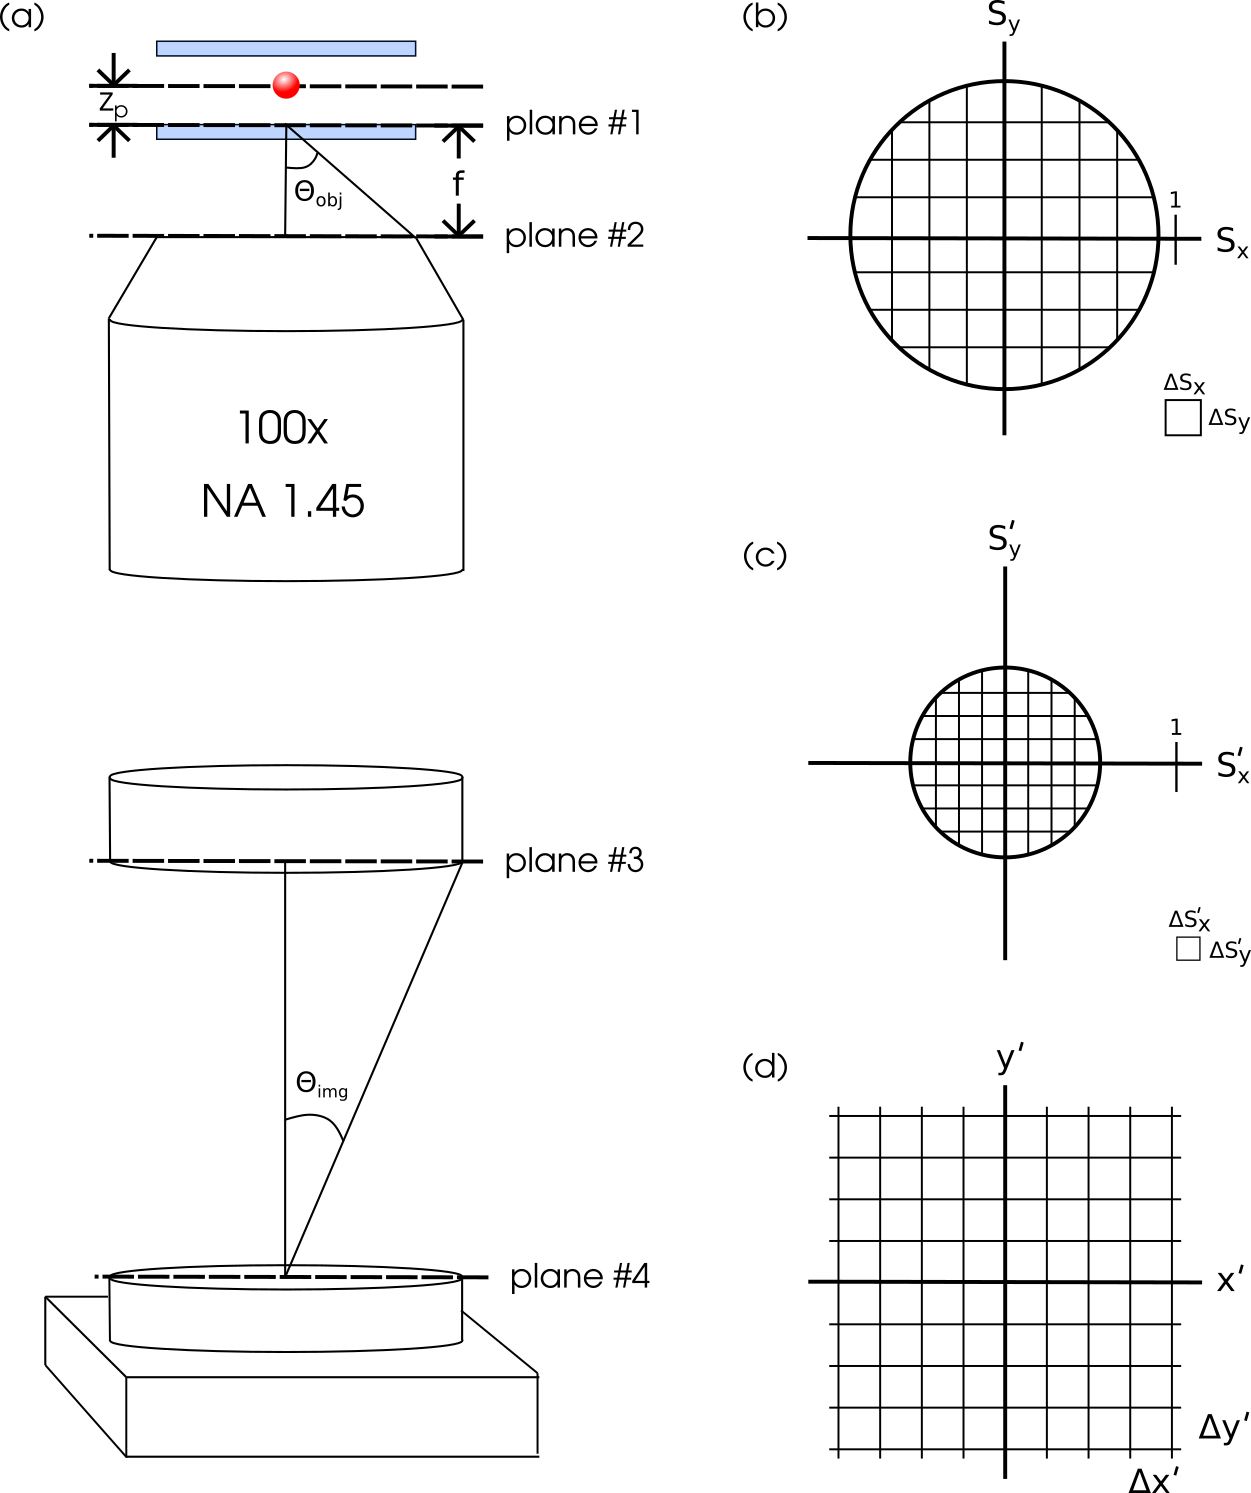
\includegraphics[width=0.95\textwidth]{debyewolf_schematic}
  \caption{Diagram depicting the planes at which the fields are evaluated.
    (a) The fields propagate through the focal plane (plane \#1) of the objective,
    are collected by the objective's entrance pupil (plane \#2), focused by the tube lens (plane 3)
    and arrive at the imaging plane (plane \#4) of the camera. (b) and (c) illustrate the
    discretization of the electric field strength factor at plane \#2 and \#3 respectively.
    (d) illustrates the discretization of the electric field at the imaging plane, plane \#4.}
  \label{fig:debye_schematic}
\end{figure}

\section{Modeling the optical train}

With the exception of a coherent illumination source, our holographic microscope
can be reduced to the four essential components of a conventional microscope:
the sample, an objective, a tube lens, and a camera. In the previous chapter,
we described the scattering of a plane wave by a spherical scatterer up to
the focal plane of the objective. We will now evaluate the scattered field and
the plane wave at several interfaces as they propagate along the optical axis
to the camera plane. Figure \ref{fig:debye_schematic}(a) illustrates the four planes
of interest. In the following sections, we will perform the following calculations
for the scattered field:
\begin{enumerate}
\item Evaluate the electric field strength factor for the scattered field at
  the entrance pupil of the objective, plane \#\num{2}.
\item Account for the axial displacement of the particle away from the focal
  plane of the objective.
\item Compute the electric field strength factor at the exit of the tube lens, plane \#3,
  by accounting for the angular demagnification imposed by the objective.
\item Use a near-field-to-far-field transform to determine the scattered
  fields at the imaging plane of the camera, plane \#4.
\end{enumerate}
Figure \ref{fig:debye_schematic}(b) presents the geometries used to define the
fields at the entrance pupil of the objective, at the tube lens, and at the camera's
imaging plane, planes \#\num{2}, \#\num{3}, and \#\num{4}, respectively.
The linearity of our optical system allows us to consider the incident field
and scattered field separately. We will derive the transformations for the
scattered field first and then summarize the corresponding transformation for the
plane wave.

\subsection{Scattering to the entrance pupil}

In \autoref{ch:hvm}, we computed the fields resulting from the scattering of
a plane wave by a homogeneous sphere embedded in an otherwise
homogeneous medium. As depicted in Fig.~\ref{fig:debye_schematic}(a), we
propagate the radially expanding scattered fields through the focal plane (plane \num{1} in
Fig.~\ref{fig:debye_schematic}) and onward to the objective's entrance pupil a distance
$z_p + f$ below the particle, where $f$ is the focal length of the objective.
\begin{figure}
  \centering
  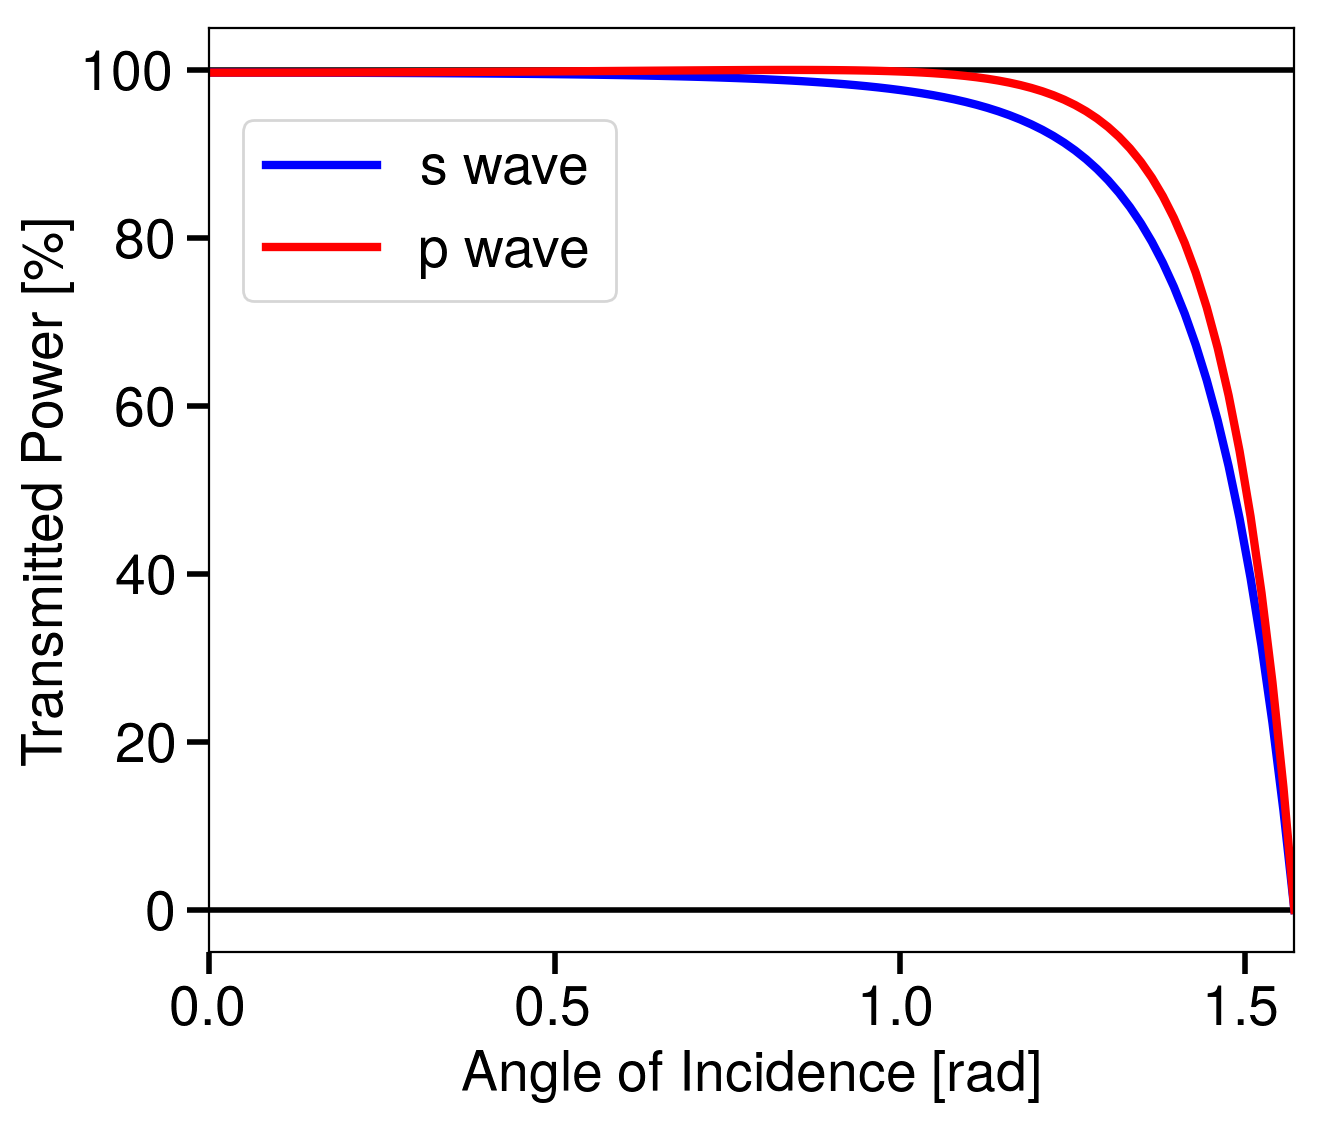
\includegraphics[width=0.7\textwidth]{waterglass}
  \caption{The Fresnel transmission coefficients for $s-$ and $p$-polarized
  waves refracting through a water-glass interface.}
  \label{fig:waterglass}
\end{figure}

During this transit, the fields reflect and refract at the water-glass interface as they
exit the sample volume. Fig.~\ref{fig:waterglass} presents the Fresnel transmission
coefficients for rays incident on the interface at angle $\theta$.
Because the scattered fields we record are dominated by low-angle scattering,
we safely neglect the reflection and refraction at this interface. Furthermore,
because we utilize an
oil-immersion objective whose refractive index, $n_{\text{oil}}$,
nearly matches that of glass, we also neglect the secondary refraction at the
glass-oil interface treated by Ovryn and Izen \cite{izen00}.

Our objective  (Nikon Plan Apo, $\num{100}\times$, numerical aperture $\num{1.45}$,
oil immersion) was manufactured to have a parfocal length of $\SI{135}{\um}$.
At this distance, wavelength, and particle size, the scattered field is in the far-zone,
also known as the Fraunhofer zone, given by $z_p + f >> a_p^2/\lambda$. In this
regime, the wave's radial dependence can be factored out from its angular dependence,
\begin{equation}
  \label{eq:strength_factor}
  \vec{E}_s(r, \theta, \phi) \approx  \vec{E}_s(\theta, \phi) \frac{e^{ikr}}{r}.
\end{equation}
The term $\vec{E}_s(\theta, \phi)$ is known as the strength factor and
depends only on the polar angle $\theta$ and the azimuthal angle $\phi$.
% FIXME: Maybe you want to see it encapsulates the electric fields angular dependence?
For computational ease, we parameterize the strength factor as $\vec{E}_s(s_x, s_y)$
with the direction cosines $s_x=\cos{\phi}\sin{\theta}$ and $s_y = \sin{\phi}\cos{\theta}$.

Casting the scattered field in terms of its strength factor will simplify
several of the upcoming calculations. Equation~\eqref{eq:strength_factor} however
is only valid when the scattered field is in the far-field regime.
Ovyrn and Izen\cite{izen00} estimate that adopting this approximation induces a maximum
$\SI{2}{\percent}$ error in the calculated intensity in the range of particle
sizes and locations that we consider here. %% FIXME: Check this claim and possible add a reference
% to an appendix that justifies these claims.

\begin{figure}
  \centering
  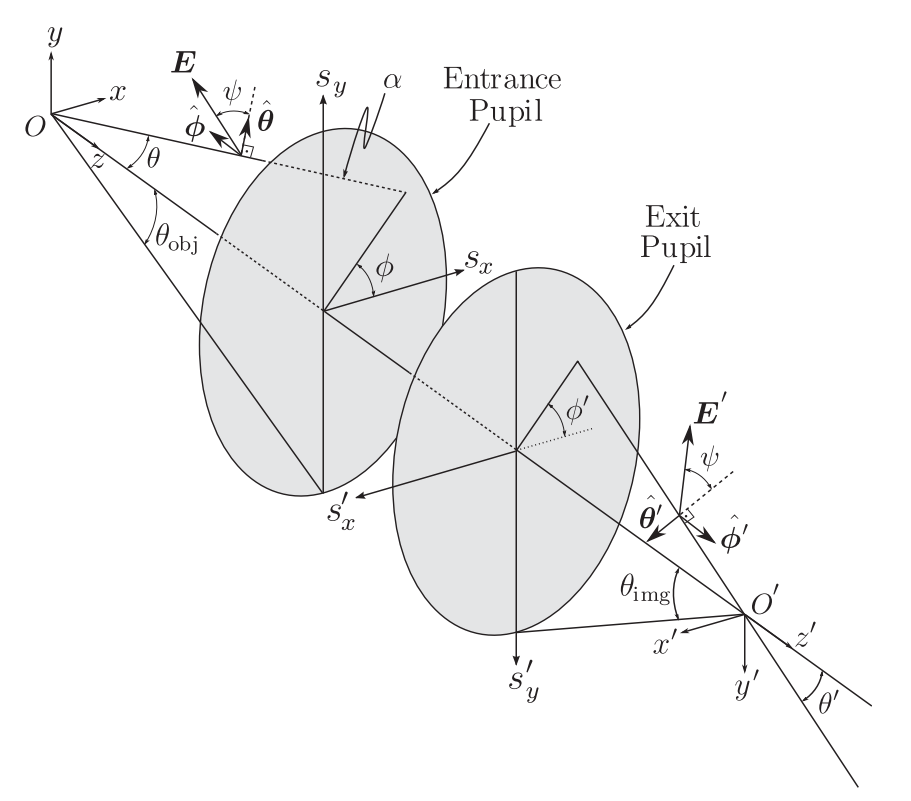
\includegraphics[width=0.75\textwidth]{debye_geom}
  \caption{The two spherical geometries necessary for our description. The un-primed coordinates
    describe the spherical geometry for waves entering the entrance pupil; the primed coordinates
    describe the spherical geometry for waves exiting the tube lens. $\theta_{\text{obj}}$ and
    $\theta_{\text{img}}$ maximal half-angle of the cone of light that can enter or exit
    the objective lens and tube lens, respectively (Ref. \cite{capoglu12}, Fig. 13).}
  \label{fig:debye_geom}
\end{figure}

\subsection{ Displacement of the scattered field}

The electric field strength factor, $\vec{E}(\theta, \phi)$, is independent
of distance and will be assumed to be originating from
the origin of the focal plane in the near-field-to-far-field transform rather
than the particle's location a distance $z_p$ above.
Following Goodman\cite{goodman05}, we account for the scatterer's displacement
along the optical axis with a relative phase shift\footnote{The sign convention used here is appropriate for a scattered positioned a distance $z_p$ in the $-\uvec{z}$ direction.}.
\begin{equation}
  \label{eq:entrance_pupil}
    \vec{E}_s(\theta, \phi)|_{\text{scatterer plane}} \approx \vec{E}_s(\theta, \phi)|_{\text{focal plane}} e^{-i\frac{2\pi}{\lambda}z_p\cos{\theta} }.
  \end{equation}

%The scattered field above gives an electric field strength factor that
%emanates from the origin of its coordinate system. In the eyes of the
%collection step, this will mean that the scatterer is located at the origin
%of the focal plane. The scatterers we hope to investigate will be staged 
%some distance z above the focal plane such that the interefence patterns 
%culiminating in the camera plane will be maximally-information dense.

%Note, we will later adopt the direction cosines $(s_x, s_y)$ used in

\subsection{Collection}
In its transit through the optical train from plane \#2 to the camera plane \#3, 
the scattered field experiences an angular demagnification 
that imparts a scaling, polarization rotation, and lensing effect.
The overall effect can be accounted for by
a coordinate transformation governed by the Abbe sine condition and by scaling
each ray to obey the conservation of energy.

The Abbe sine condition,
\begin{equation}
  M = \frac{n_m \sin \, \theta}{n^{\prime} \sin \, \theta^{\prime}}
  \label{eq:abbe_sine}
\end{equation}
is necessary for sharp imaging \cite{capoglu12} and is rigorously
satisfied in modern optical designs.
Here, $M$ is the system's lateral magnification, $n_m$ is the medium's refractive index,
and $n'\approx 1$ is the refractive index at the camera plane.
A ray entering the objective lens at angle $\theta$ relative to the optical axis exits
the tube lens at an angle $\theta^{\prime}$ with a polarization rotation of
$\SI{180}{\degree}$ as portrayed in Fig.~\ref{fig:debye_geom}.
Additionally, angular demagnification concentrates the electromagnetic radiation
to a smaller solid angle and increases the magnitude of the electric field strength
factor. Accounting for these three effects, we relate the electric field strength at the
entrance pupil of the objective to the electric field strength at the tube lens as
  \begin{equation}
    \begin{split}
    \vec{E}_s'(\theta', \phi')\cdot\hat{\theta'} & = - M \sqrt{ \frac{n'\cos{\theta'}}{n\cos{\theta}}}\vec{E}_s(\theta, \phi)\cdot\hat{\theta} \hspace{0.2 in}\text{and}\\
    \vec{E}_s'(\theta', \phi')\cdot\hat{\phi'} & = - M \sqrt{ \frac{n'\cos{\theta'}}{n\cos{\theta}}}\vec{E}_s(\theta, \phi)\cdot\hat{\phi}.
    \end{split}
  \end{equation}

For computational ease, we again adopt direction cosines $s'_x = \cos \, \phi'\sin \, \theta'$ and
$s'_y=\sin{\phi'}\sin{\theta'}$ such that the electric field strength
factor exiting the tube lens is parameterized as $\vec{E}_s^{\prime}(s'_x, s'_y)$. Under this
coordinate transformation, the Abbe sine condition given by Eq.~\eqref{eq:abbe_sine} can
readily be seen as a linear scaling of the magnitudes of the direction cosines

\begin{equation}
  M = \frac{n_m \sqrt{s_x^2 + s_y^2 }}{n^{\prime} \sqrt{s_x^{\prime 2} + s_y^{\prime 2} }}.
\end{equation}
  
\subsection{Refocusing the fields to the camera plane}
Finally we utilize a near-field-to-far-field transform to propagate the scattered
field from the tube lens to the imaging plane.
The Debye-Wolf diffraction integral transforms the electric field strength factor at a lens
surface to the scattered field, $\vec{E}_{s,\text{img}}$, present in the focal plane of that
lens:
\begin{equation}
  \vec{E}_{s,\text{img}}(x', y') = \frac{i k'}{2 \pi} \iint_{\Omega_{\text{img}}} \vec{E}_s'(s'_x, s'_y) \frac{e^{-ik'(s'_xx'+s'_yy')}}{\cos{\theta'}}ds'_xds'_y 
  \label{eq:debyewolf}
\end{equation}
where $k'$ is the wavenumber in the medium above the camera and $\Omega_{\text{img}}$
is the domain of integration set by the Abbe sine condition and the condition
that $s_x^2+s_y^2 \le \text{NA}/n_{\text{oil}}$. Note that $\cos \, \theta' = \sqrt{ 1 - (s_x^{\prime 2} + s_y^{\prime 2} )}$. Several points are worth mentioning:
\begin{enumerate}
\item This integral acts as an inverse of Huygen's principle; a spherical wave is
  decomposed into a multitude of plane waves whose phase relations and subsequent
  interference produce the same effect as the original spherical wave.
\item The Debye-Wolf transformation takes $\vec{E}'$, a strength factor with units
  $\si{\volt\meter}$, defined in spherical coordinates on plane \#\num{3} and
  returns the electric field  in cartesian coordinates in plane \#\num{4}.
\item The transformation appears to be distance agnostic; the distance
  between plane \#\num{3} and \#\num{4} never explicitly appears. However the domain
  of integration, $\Omega_{\text{img}}$, is limited by the Abbe sine condition
  such that the planes \#\num{3} and plane \#\num{4} must be separated by $M \, f$.
\end{enumerate}

The Debye-Wolf integral can account for phase aberrations, $\Phi(s'_x,s'_y)$,
due to imperfections in the optical train.
To do so, the integrand of the Debye-Wolf integral is multiplied by a phase term
$e^{ik'\Phi(s'_x,s'_y)}$. We will not consider aberrations, however, because
the goal of this study is to access limitations in hologram formation
under ideal conditions.

%Several points are worth mentioning:
%\begin{enumerate}
%\item The Debye Wolf integral takes a field strength factor $\vec{E}_s'$,
%  an integration domain $\Omega_{img}$ and the wavenumber $k'$ as its inputs.
%  From these inputs, the electric field in the (x'-y') plane is
%  calculated. 
%\item Heuristically, one should imagine that $\Omega_{img}$ dictates how far 
%  away the plane $(x'-y')$ will be (the distance scales with the size of 
%  $\Omega_{img}$), that $k'$ gives the field strength factor the necessary 
%  units to become an electric field and the electric field strength factor 
%  contains most of the information detailing the interference pattern in the
%  x'-y' plane ($k'$ has influence here as well).
%\item This integral in many ways amounts to
%  an inverse of Huygen's rule; a spherical wave is decomposed into a multitude 
%  of plane waves whose phase relations and subsequent inteference produce
%  the same effect as the original spherical wave.
%\item The Debye-Wolf formalism easily accounts for any phase aberration 
%  $\Phi(s'_x,s'_y)$ of the field as it passes through the optical train. To do so, the integrand
%  of the Debye-Wolf integral is multiplied by a phase term $e^{ik'\Phi(s'_x,s'_y)}$.
%\end{enumerate}

With the exception of the $k'$ in the phase term and the $\cos{\theta'}$ 
modifying the differential element, we should recognize the
Debye-Wolf integral as a Fourier transform. We will discretize this
Fourier transform subject to sampling and aliasing conditions described
in the appendix \ref{app:discretize_dw}. Here we summarize and interpret the result:
\begin{equation}
  \begin{split}
    \vec{E}_{s,\text{img}}( m \Delta_x, n \Delta_y) & \approx \frac{i k' \Delta s'_x \Delta s'_y}{2 \pi} e^{-i2\pi \left ( \frac{s'_{x_o}}{\Delta s'_x N_p} m + \frac{s'_{y_o}}{\Delta s'_yN_q} n \right ) } \vec{E}_s'\left [ m, n \right ] \\
    \vec{E}_s'\left [ m,n \right ] & = \sum_{p=0}^{N_p-1}\sum_{q=0}^{N_p-1}\vec{G}'\left [p,q\right ] e^{-i2\pi \left ( \frac{pm}{N_p}+\frac{qn}{N_q} \right ) } \\
    \vec{G}'(s'_x,s'_y) & \doteq \vec{E}'_s(s'_x,s'_y)\frac{\vec{E}'_s(s'_x,s'_y)}{\cos{\theta'}}e^{-ik'\Phi(s'_x,s'_y)}
  \end{split}
  \label{eq:complete_dw}
\end{equation}
where the the $s_x'$-$s_y'$ plane is discretized into a
$N_p$ by $N_q$ grid with a sampling period $\Delta s_x'$ along the $s_x'$ axis and
$\Delta s_y'$ along the $s_y'$ axis, and the $x'$-$y'$ plane is similarly discretized with
sampling periods $\Delta x$ and $\Delta y$.
The sampling periods are inversely related such that $\Delta_x = 2\pi \, / \, k' \Delta s_x' N_p$
and $\Delta_y = 2\pi \, / \, k' \Delta s_y' N_p$.
Note that the vector functions with parens encasing their arguments represent
continuous functions whereas those with square brackets encasing their arguments represent
discrete approximations of continuous functions.

The Debye-Wolf integrand rapidly oscillates with respect to its arguments $s_x'$ and $s_y'$.
To ensure our approximation to the integral \eqref{eq:debyewolf} converges, we
must appropriately sample the $s_x'$-$s_y'$ grid. In addition, we must mitigate any
aliasing that may result from the Fourier transform in Eq.~\eqref{eq:complete_dw}.
Further restricting our discretization scheme, the sampling periods $\Delta_x$
and $\Delta_y$ should be comparable to the size of a pixel. These competing constraints
can be cast as an integer equation and approximately solved as demonstrated
in appendix \ref{app:discretize_dw}.

\subsection{Superposition of the propagated fields}

The propagation of the incident plane wave through the optical system is more easily explained.
The incident field travels parallel to the optical
axis towards the entrance pupil of the objective. The objective
and tube lens then laterally magnify the incident field and induce a
$\SI{180}{\degree}$-shift in phase.
The incident field maintains its polarization and arrives at the imaging plane as
\begin{equation}
  \vec{E}'_{\text{inc}}(x',y') = -\frac{1}{M}\sqrt{\frac{n_1}{n_2}} \vec{E}_{\text{inc}}(x,y).
\end{equation}
The image in the camera plane is then
\begin{equation}
  I(x', y') = \preint \left | \vec{E}'_{\text{inc}}(x',y') + \vec{E}'_s(x', y') \right |^2.
\end{equation}

  
\section{Comparison to Scalar Diffraction Theory}

Having accounted for the propagation of the incident field and the scattered
field through the optical system, we are now ready to assess differences
between the vector theory and the scalar theory. As shown in Fig.~\ref{fig:debye_difference_ps},
the two theories produce nearly identical holograms for a \SI{1.0}{\um} diameter
polystyrene particle with refractive index $n_{\text{p}}=1.59$ displaced
\SI{13.5}{\um} above the focal plane; the difference in intensity at each
pixel in the respective holograms is well below the sensitivity of our camera.


\begin{figure}
  \centering
  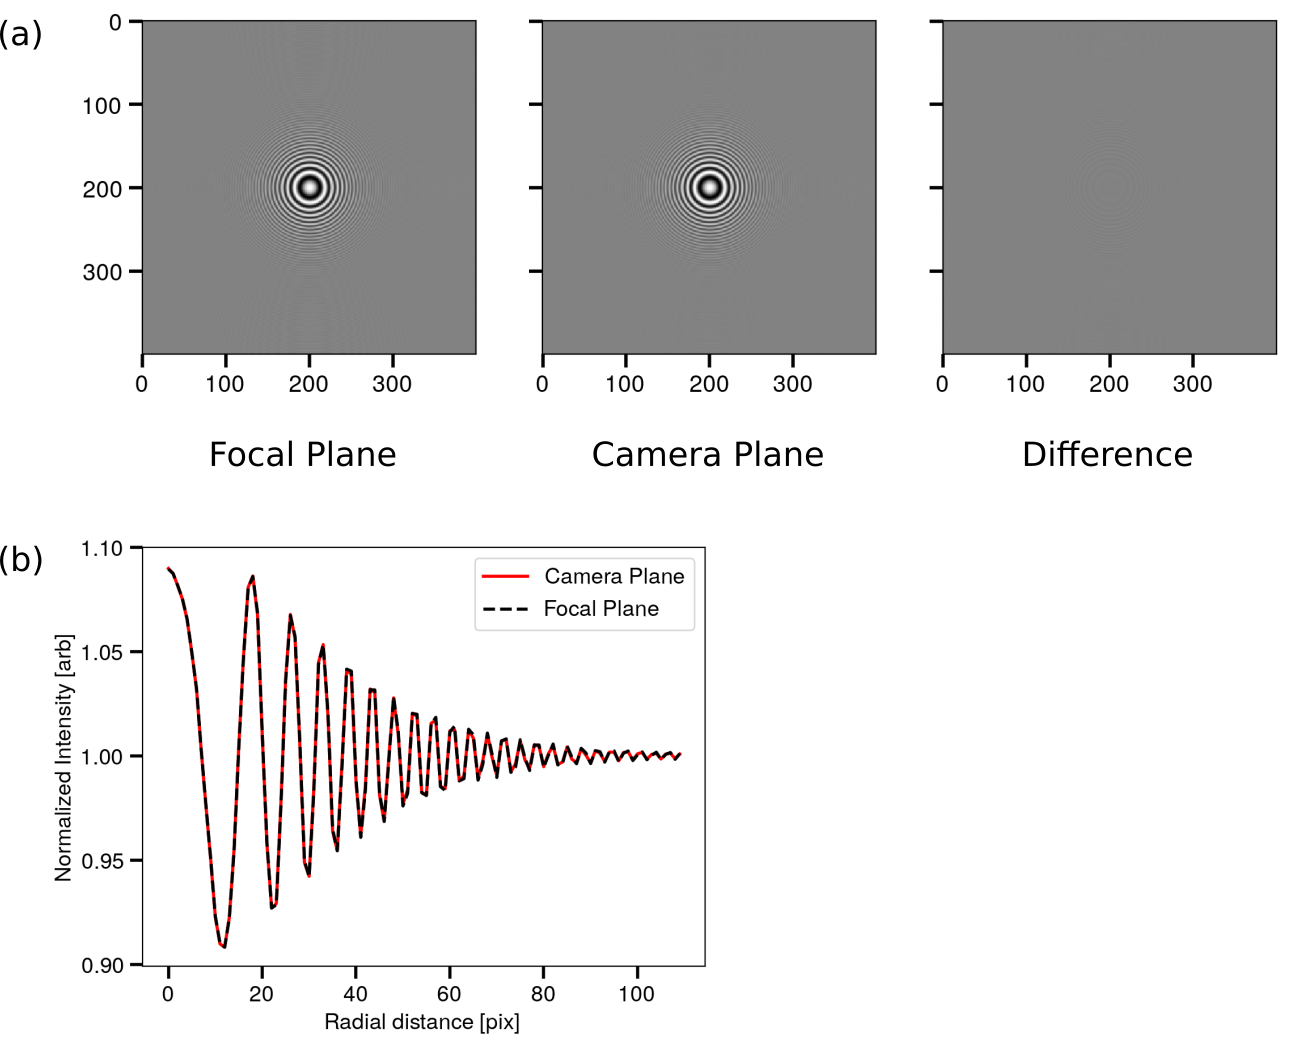
\includegraphics[width=\textwidth]{debyewolf_differences}
  \caption{(a) Holographic images produced in the focal plane of the objective lens and
    the imaging plane of the camera, and an image of their differences.
    (b) Radial profiles of holographic snapshots taken
    in the focal plane of the objective and the imaging plane of the camera.
    These particular holographic features were produced by a $\SI{1.0}{\um}$
    diameter polystyrene particle $\SI{13.5}{\um}$ above the focal plane.}
  \label{fig:debye_difference_ps}
\end{figure}

To systematically assess the differences in the two theories,
we use Eq.\eqref{debyewolf} to synthesize holographic
images as they would appear in the camera plane. Synthetic holograms
were computed for spheres with radii ranging from
$a_{\text{p}}=\SI{0.5}{\um}$ to $\SI{5}{\um}$, refractive indexes from
$n_{\text{p}}= \SI{1.4}{}$ to $\SI{1.8}{}$, and displacements from the focal plane,
$z_{\text{p}}=\SI{5}{\um}$ to $\SI{50}{\um}$.
We then fit each synthetic hologram to the scalar theory representing
images in the focal plane of the objective lens, as described
in \autoref{ch:hvm}. The degree to which the resulting fit parameters differ
from the known scatterer properties set a lower bound for the error of adopting
the scalar theory in favor of the vector theory.

Over the majority of parameter space, the error in diameter and
axial displacement are bounded by $\SI{1}{\nm}$ while the error
in refractive index is bounded by $\SI{0.001}{}$; in all three
parameters, the maximum error is less than the reported resolution of
the technique \cite{krishnatreya14}. In certain regions of parameter
space, our discretization scheme could not sufficiently sample the
highly-oscillatory integrand in Eq.~\eqref{eq:debyewolf}.
No synthetic holograms are available in this range.

\section{Discussion}

This chapter provides a detailed treatment of the scattered field
and incident field as they propagate through the optical train to the camera
to produce an image.
We determined that the image accounting for
the effects of refraction, reflection, lateral magnification, and angular
demagnification does not change the resulting hologram by a measurable amount.
The existing formulation therefore is optimal in this sense. Additionally the computational complexity of producing
the image in the camera plane greatly exceeds that of producing the
image in the focal plane; for this reason, we recommend the use of the
scalar theory in fitting experimental holograms with ideal optics.
For real lenses, some degree of phase-aberrations are imparted by
the optical train; in the case of non-ideal holographic imaging,
our theory provides a model which accounts for phase-aberrations,
including spherical aberrations.


%For certain optical limitations, such as low-NA imaging \cite{saglimbeni16},
%the image in the focal plane can be successfully modified without a theory
%explaining the propagation of fields through the optical train.
%Our formalism accommodates phase-aberrations caused by the optical train
%and can be used to model holographic images produced with non-ideal optics.



    \newpage
    
    \chapter{Characterizing imperfect colloidal spheres}
\label{ch:dimpled}

\section{Introduction}
In developing the theory of holographic particle characterization, we have modeled
colloidal particles as homogeneous
dielectric spheres. Many naturally-occurring and synthetically-made particles
resemble this ideal because surface tension favors the formation of spheres.
For such particles, the Lorentz-Mie model introduced in \autoref{ch:hvm} is a
good description. Many other kinds of particles however, are not spherical and
are not homogeneous. This chapter address how departures from sphericity
affect the results of holographic characterization.

We present a series of experimental and simulated results from fitting
holographic features of imperfect spheres with the Lorenz-Mie theory.
Our work demonstrates that holographic particle characterization
can measure the size and refractive index
of imperfect spheres with nearly the same precision as for the ideal
case, provided that their
deviation from sphericity is not too pronounced. 

\begin{figure*}[t]
  \centering
  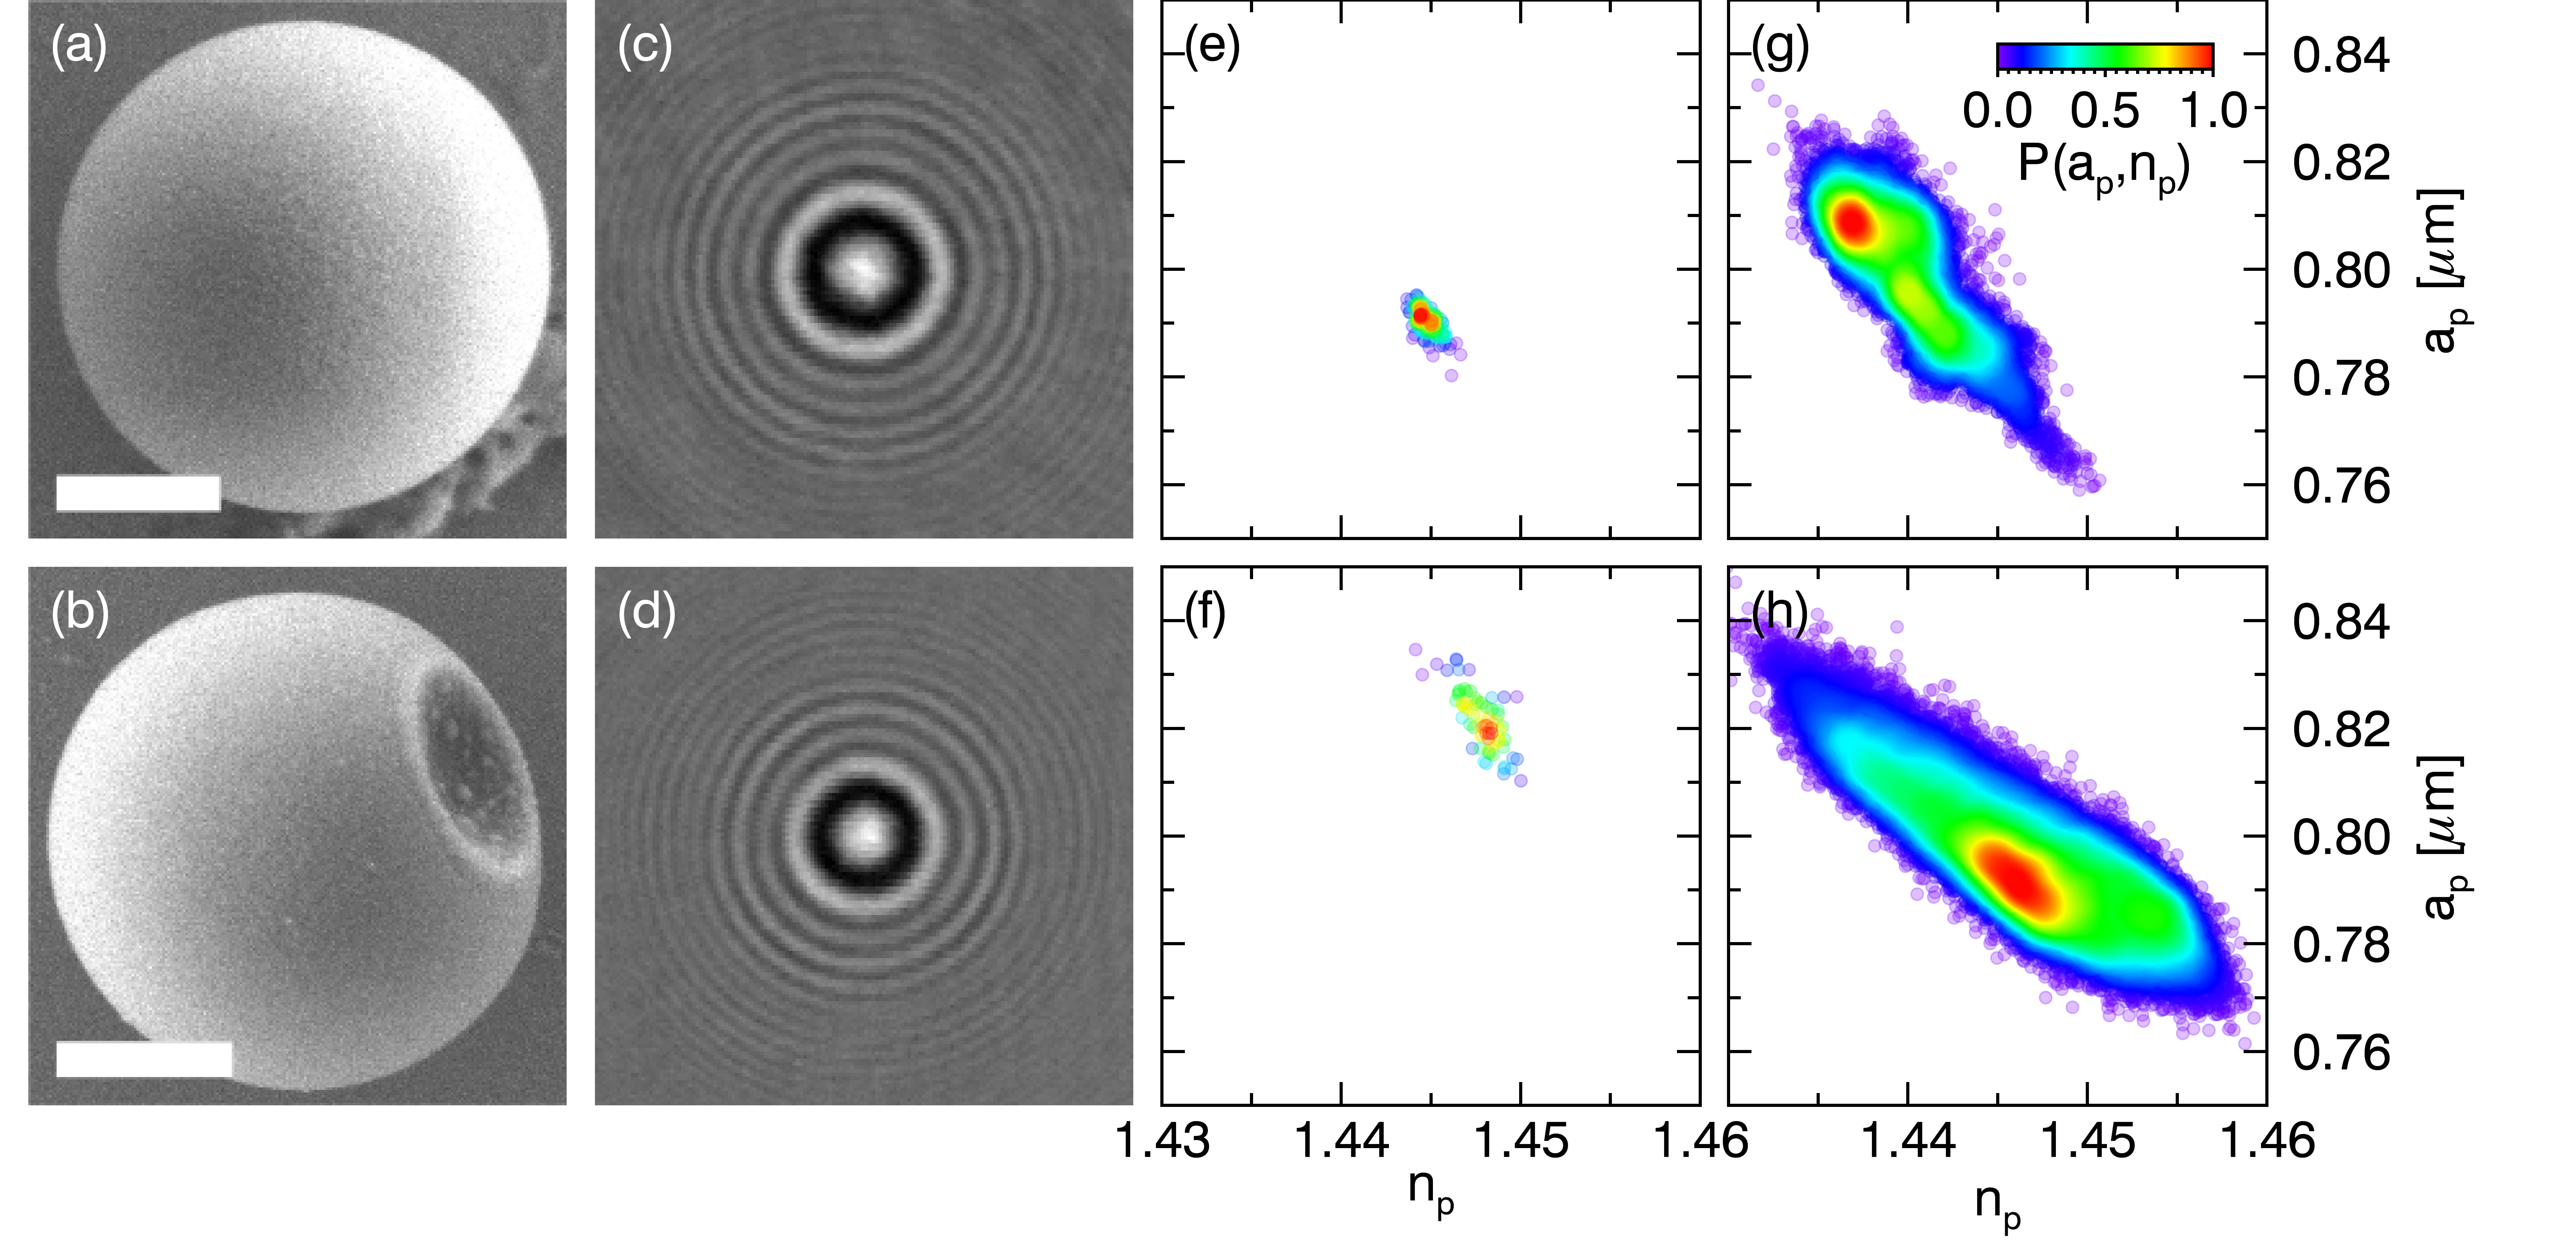
\includegraphics[width=\textwidth]{dimpled_figure1}
  \caption{(a) Scanning electron micrograph of a colloidal TPM sphere and 
    (b) a dimpled sphere.  Scale bars represent \SI{500}{\nm}.
    (c) and (d) Corresponding holograms for
    particles from the samples show in (a) and (b).  (e) \num{5000} measurements
    of sphere radius and refractive index for a single
    TPM sphere held in an optical tweezer.  Each point represents
    a single measurement, and is colored according to the
    relative density of measurements, $P(a_p,n_p)$.  (f) equivalent result for
    a dimpled sphere.  (g) \num{5000} measurements of the radius and
    refractive index of a freely diffusing sphere.  (h) Equivalent
    result for a dimpled sphere \cite{hannel15}.
   }
  \label{fig:singleparticle}
\end{figure*}

\section{Synthesizing TPM particles}

To experimentally investigate the effect of modeling aspherical scatterers
as spheres, we synthesize three populations of colloidal particles: ideal spheres,
spheres with a small dimple, and spheres with a large dimple.
Each population is analyzed with HVM by using the Lorenz-Mie theory
for scattering by a sphere.

Our model system for this work consists of monodisperse
colloidal particles synthesized through emulsion polymerization of
3-methacryloxypropyl trimethoxysilane (TPM) \cite{sacanna13}.
Depending on how they are made, these particles can take the form
of spheres, as shown in Fig.~\ref{fig:singleparticle}(a), or dimpled
spheres, as shown in Fig.~\ref{fig:singleparticle}(b), in which both
the sphere radius and dimple dimensions are drawn from narrow
distributions. 

Ideal spheres and dimpled spheres are synthesized through similar pathways.
TPM oil, which ordinarily is insoluble in water,
undergoes hydrolysis in a basic environment (pH $> 9$) and becomes
water soluble.
Solubilized monomers then form insoluble oligomers,
which condense into spherical droplets.
Once the droplets are fully grown, they are solidified through
free radical polymerization that is initiated by adding 
$2,2^\prime$-azo-bis-isobutyrynitrile (AIBN) and 
heating to \SI{80}{\degreeCelsius} for 
\SI{2}{\hour}.
The particles then are washed and redispersed in deionized water
for study.

Homogeneously nucleated TPM droplets form spheres.
To synthesize dimpled spheres, we heterogeneously nucleate
droplet condensation by adding \SI{0.65}{\um}-diameter
polystyrene spheres to the aqueous phase.
These small spheres serve as nucleation sites for TPM condensation and remain
embedded in the surface of the resulting droplet to a depth that
depends on their wetting characteristics.
They remain in place during polymerization, and thus
determine the size of the dimple in the final particle. 
After the TPM is polymerized, the polystyrene spheres are
dissolved by transferring the particles into toluene, leaving
uniformly sized dimples.
For the sample represented by Fig.~\ref{fig:singleparticle}(b), the
dimple accounts for \SI{5}{\percent} of the equivalent sphere's
volume, as estimated from scanning electron microscopy images.
The completed particles are then transferred back into 
deionized water for cleaning and study.

Dimpled spheres have immediate applications for lock-and-key
colloidal self-assembly
\cite{sacanna10,macfarlane10,sacanna11,ashton13,phillips14,wang14} 
and are models for colloidal microcapsules \cite{chang64}, which are widely
used in industrial applications, and tend to buckle into dimpled spheres
through osmotic stress \cite{chang64,knoche11,jose14}. 
These model particles are useful for assessing the limits of holographic
characterization because their departure from sphericity is well defined.

\section{Characterizing Spherical and Aspherical Colloidal Particles}

We prepared samples for holographic characterization
by diluting their respective stock dispersion in water to a volume fraction of
\num{e-5} and introducing the diluted dispersion into a \SI{50}{\um}-thick gap between a
glass microscope slide and a cover slip. Particles were translated into the
observation volume for recording under quiescent conditions. 

Their holograms were then analyzed with the Lorenz-Mie model, treating each
particle as if it were a sphere.
Each fit yields an estimate for the particle's three-dimensional position $\vec{r}_p$,
its radius $a_p$ and its refractive index $n_p$.
The data in Fig.~\ref{fig:singleparticle}(e) show results obtained for
a typical TPM sphere localized in an optical trap that was
projected through the microscope's objective lens using the
holographic optical trapping technique \cite{dufresne98,grier03}.
The spread in values is comparable to the numerically
estimated uncertainty in the individual fits,
$a_p = \SI{0.790(3)}{\um}$ and $n_p = \num{1.445(1)}$,
suggesting both that
the imaging model is appropriate, and also that the signal-to-noise
ratio estimated by the median-absolute-deviation (MAD) metric
is reasonable.
This sphere's holographically measured radius is consistent with the 
mean value, \SI{0.76(6)}{\um}, obtained through SEM observations 
on the same batch of spheres.
The polymerized particles' refractive index is larger 
than that of monomeric TPM oil, \num{1.431} at the imaging wavelength.

The scattering function for an aspherical object, 
such as a dimpled sphere, depends on the object's detailed shape
and orientation \cite{mishchenko02}.
Analytical results are available for just a few special cases.
For more general cases, numerical methods are required, 
such as the discrete dipole approximation (DDA) \cite{draine94}. 
Even with highly optimized implementations \cite{yurkin11}, however,
such approaches are computationally intensive \cite{fung12,perry12,wang14using}.
If an object's departure from sphericity is small enough, and if the
influence of the non-ideality on the recorded hologram is sufficiently well
localized within the recorded image, Lorenz-Mie analysis
may still yield useful results for the particle's
size and refractive index without incurring this cost.

Figure~\ref{fig:singleparticle}(f) shows results obtained by fitting the
ideal-case model to holograms of an optically trapped dimpled sphere.
The radius estimated by straightforward 
Lorenz-Mie analysis of \num{60} such holograms
is \SI{0.821(6)}{\um}.
The corresponding estimate for the refractive index,
\num{1.448(1)} is remarkably similar to the value obtained for the
ideal spheres.
In both cases, the distribution of
values extracted from nonlinear least-squares 
fits to Eq.~\eqref{eq:gen_norm} with the scattered field provided
in Eq.~\eqref{eq:scatteredfield} is consistent with single-fit error estimates.
This agreement suggests that the ideal model can yield quantitative
results for the characteristics of dimpled spheres, without incurring
the costs of more realistic modeling.

SEM analysis suggests that the sample-averaged radius of the
dimpled spheres is \SI{0.75(5)}{\um}, which is slightly smaller
than the result obtained holographically.
Similar discrepancies have been noted in previous studies
\cite{yamada85,cermola87},
and reasonably may be explained by changes
induced by preparing the spheres for SEM observation.

The extent to which a dimpled sphere's hologram may be described
with an ideal sphere's scattering function depends on the dimple's
orientation.
Optically trapping a dimpled sphere constrains its rotations 
as well as its translations, fixing the dimple's axis in the
transverse plane.
When released from its trap, the dimpled sphere rotates freely in three
dimensions, with consequences for holographic characterization.
Figure~\ref{fig:singleparticle}(g) shows the distribution of characteristics
obtained over the course of \SI{10}{\minute} for a freely diffusing
sphere.
The mean radius and refractive index obtained for this particle are
\SI{0.80(1)}{\um} and \num{1.440(3)}, respectively.
Additional uncertainty in the particle's radius and refractive index
reflects uncorrected interference artifacts in the recorded hologram due
to defects in illumination \cite{krishnatreya14}.
The corresponding distribution for the freely diffusing dimpled sphere
is broadened still further, and displays a strong anticorrelation between
radius and refractive index.
The peak of this distribution remains at the trapped-particle values,
$a_p = \SI{0.80(1)}{\um}$ and $n_p = \num{1.447(5)}$,
presumably because the randomly oriented particle is more likely 
to have its dimple transverse to the optical axis than facing it.

Having the dimple pointing sideways is beneficial for holographic
characterization.  In this orientation, the dimple's contribution to the 
scattering pattern is asymmetric, and thus minimally influences the
fit to the largely symmetric model.  It plays a role comparable to
uncorrected background artifacts, reducing the precision, but not
seriously affecting the mean values.
When the dimple is directed along the axis, however, distortions to
the scattering pattern are symmetric about the axis and thus affect
the fits more strongly.


The success of an idealized model for describing light scattering by a
dimpled sphere may be explained at least heuristically by treating
the dimple as a volume of the sphere whose scattering is phase-shifted
by \SI{180}{\degree}.
The scattering amplitudes for the sphere as a whole and for the dimple
scale roughly as their respective volumes.
If the dimple's volume is only a small fraction of the
sphere's, and if, furthermore, the dimple's contribution is asymmetric,
the perturbation should be negligible.


\section{Determining Tolerable Asphericity}


\begin{figure}[!t]
  \centering
  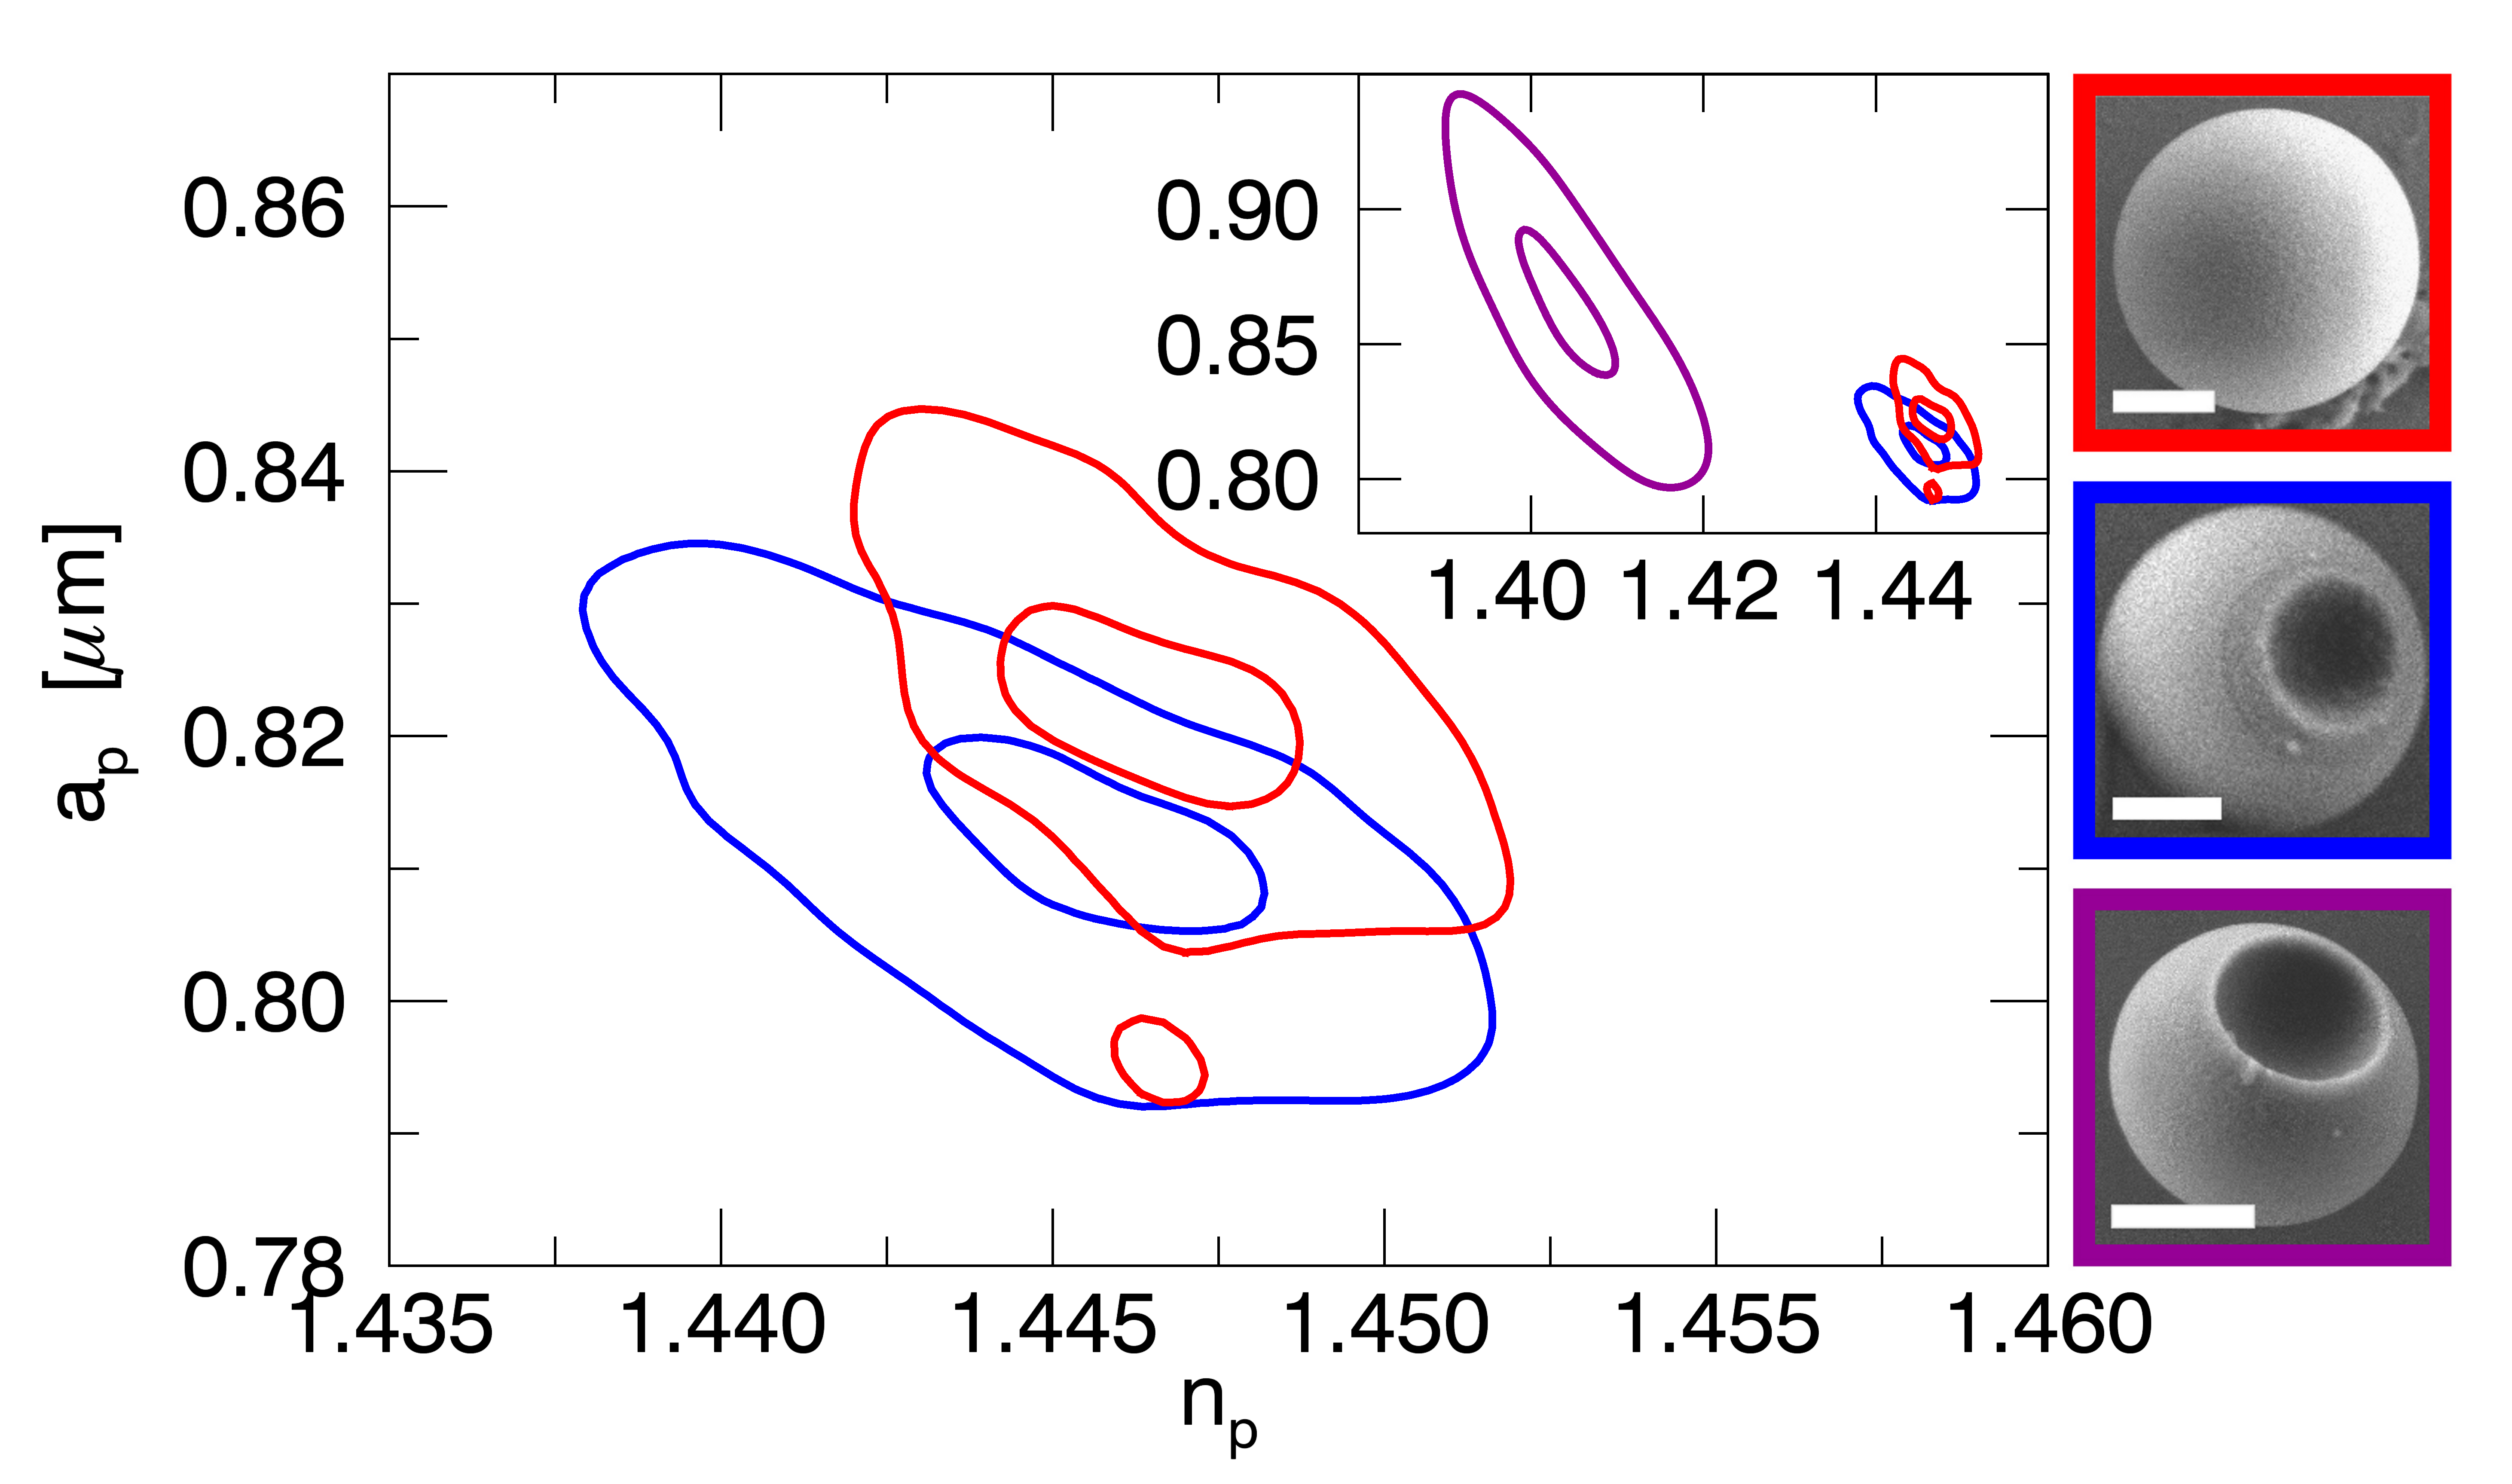
\includegraphics[width=0.9\columnwidth]{dimpled_figure2}
  \caption{Level sets of the holographically measured 
    distributions of particle properties for TPM spheres
    (red), dimpled spheres with small dimples (blue) and
    large dimples (purple).  The presence of a small dimple
    has no significant influence on holographic characterization
    results.  Larger dimples cause systematic errors.
    SEM images show typical representatives of each sample,
    with scale bars denoting \SI{500}{\nm} \cite{hannel15}.}
  \label{fig:distributions}
\end{figure}

We applied the same technique to characterizing the distribution
of properties in monodisperse samples of TPM spheres and 
TPM dimpled spheres.
For these measurements, dispersions of particles at a volume fraction
of \num{e-4} were streamed down a channel by a pressure driven flow
with a peak speed of $\SI{100}{\um\per\second}$.  This is fast enough
to acquire holograms of \num{5000} spheres in \SI{10}{\minute}, but
not so fast as to incur artifacts due to motion-induced blurring
\cite{cheong09,dixon11}.
Results plotted in Fig.~\ref{fig:distributions} for TPM spheres reveal
a reasonably symmetric distribution of particle sizes and refractive
indexes peaked at \SI{0.82(2)}{\um} and \num{1.446(6)}, respectively.
These values are consistent with the single-sphere measurements
reported in Fig.~\ref{fig:singleparticle}.
The corresponding distributions for dimpled spheres plotted in
Fig.~\ref{fig:distributions} become increasingly broad and asymmetric
as the relative size of the dimple increases.
Particles with \SI{5}{\percent} dimple volumes yield a mean refractive
index, $n_p=\num{1.444(6)}$, consistent with the ideal spheres' value.
The mean radius, $a_p=\SI{0.81(2)}{\um}$, is consistent with the
  single-sphere result reported in Fig.~\ref{fig:singleparticle}(h).
Increasing the dimple volume to \SI{10}{\percent} leads to
substantial deviations, with a mean refractive index of
$n_p=\num{1.42(3)}$.
Some variability can be attributed to the dimpled spheres'
random orientation in the channel.

To assess the extent of the distortions that can be handled with the
idealized model for holographic characterization, we apply the
discrete-dipole approximation \cite{draine94,yurkin11,fung12,perry12,wang14using}
to compute holograms of 
dimpled spheres, and then analyze the resulting synthetic data
with the same software used to analyze experimental data.
The discrete-dipole approximation treats an object as a three-dimensional
arrangement of independent microscopic dipole scatterers, each of which
is illuminated by the incident beam and also by the first-order scattering
of its neighbors\footnote{The ADDA implementation of the discrete-dipole approximation
\cite{yurkin11} used for this study discretizes the particle volume on a 
three-dimensional square grid with an effective lattice constant
roughly one-tenth the wavelength of light in the material.  Typical
numbers of dipoles range from \num{100} for the smallest particles
considered to \num{18000} for the largest.}.
The superposition of scattered waves yields an estimate for 
$\vec{f}_s(k\vec{r})$ that is used to synthesize a hologram.
Dimpled spheres are modeled as the superposition of
two spheres separated by a center-to-center distance $d$, one
of radius $a_p$ and refractive index $n_p$, and the other of radius
$a_d$ and the refractive index of the medium.

Analyzing DDA-generated holograms of perfect spheres yields 
excellent agreement
with input parameters for sphere radii up to $a_p \le \SI{0.5}{\um}$. 
Scattering by larger spheres requires proper treatment of higher-order scattering,
and is not supported by the ADDA implementation of the DDA algorithm
that we adopted \cite{yurkin11,wang14using}.
Limiting the analysis to parameters within the spherical particle's domain of
applicability, we assessed discrepancies between input parameters
and values obtained by fitting
the resulting holograms with the scattering function for ideal spheres.

\begin{figure}[!t]
  \centering
  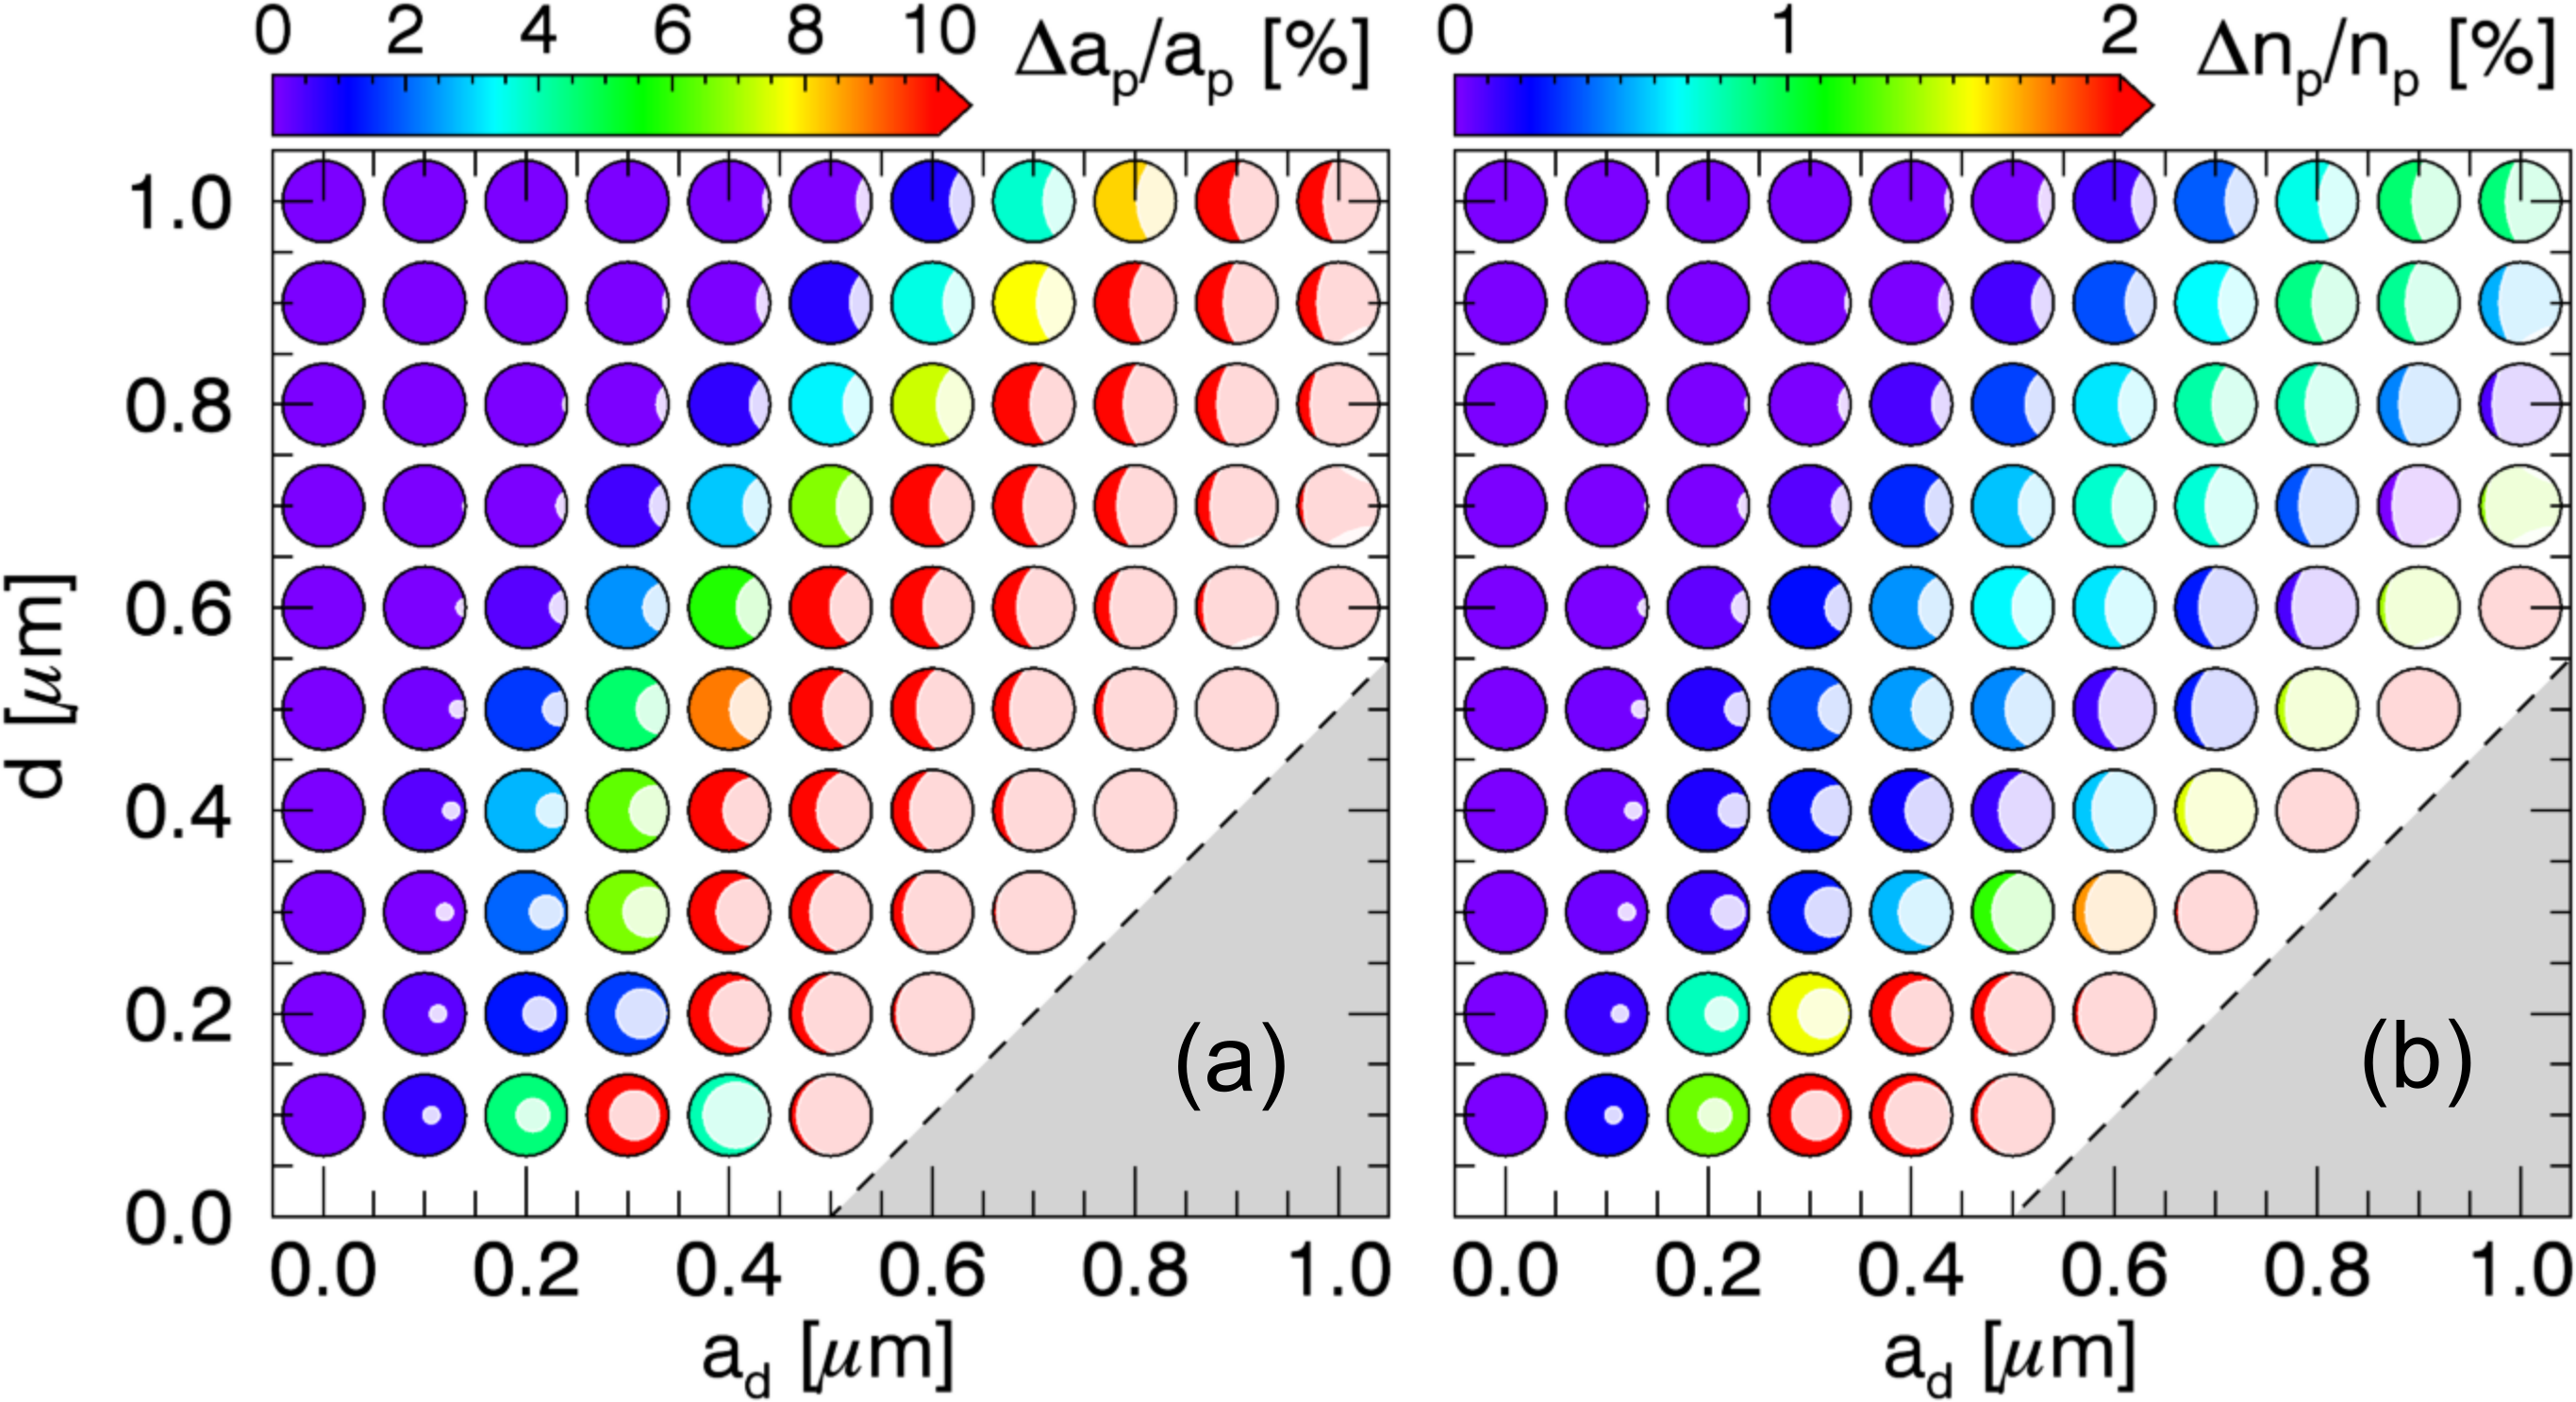
\includegraphics[width=\columnwidth]{dimpled_figure3}
  \caption{Holographic characterization of dimpled TPM spheres 
    with radius $a_p = \SI{0.5}{\um}$ as a function of dimple radius
    $a_d$ and center-to-center distance, $d$.
    (a) Relative error in holographically estimated radius.
    (b) Relative error in refractive index.
    Plot symbols indicate shape of dimpled spheres \cite{hannel15}.}
  \label{fig:dimpledperformance}
\end{figure}

Figure~\ref{fig:dimpledperformance} summarizes the performance of
Lorenz-Mie analysis for characterizing spheres bearing a single
dimple.
The colors of the plot symbols
in Fig.~\ref{fig:dimpledperformance}(a) represent the relative
error in the radius obtained by applying the Lorenz-Mie analysis
to the computed hologram of a dimpled sphere.
The plot symbols' shapes correspond to the
dimpled particles' medial profile for each value of $a_p$ and $d$.
Figure~\ref{fig:dimpledperformance}(b) shows the corresponding
results for the refractive index.
Deviations become larger for spheres distorted by larger dimples,
particularly if those dimples are aligned with the optical axis.
This leaves a substantial domain of applicability within which
computationally efficient implementations of hologram analysis
can be used to measure the properties of this class of
imperfect spheres.
As a rule of thumb, near-ideal results can be obtained for dimples
that take up no more than \SI{5}{\percent} of a sphere's volume.

The same approach also should be useful for characterizing
colloidal particles with multiple dimples, so-called colloidal golf
balls \cite{dai13},
and for colloidal snowmen \cite{chaturvedi12}
with small protrusions instead of dimples.
Simulations with up to 10 equally-sized dimples distributed
uniformly across the sphere's surface yield values for
$a_p$ and $n_p$ within \SI{1}{\percent} of the ideal values for total dimple
volumes less than \SI{5}{\percent} of the sphere's volume.
The influence of orientation becomes less pronounced as the number
of dimples increases.
Removing a larger percentage of the volume 
yields disproportionately worse results.

\section{Discussion}

The success of holographic particle characterization for analyzing
holograms of imperfect spheres helps to explain the technique's
previously documented success with real-world samples.
This study suggests that small amounts of surface roughness have
little influence on the results obtained by fitting to the theory
for light scattering by ideal spheres.
Conversely, we have demonstrated the use of the Lorenz-Mie theory
as an effective sphere model for aspherical particles. For micrometer
sized particles whose geometry differs modestly from a sphere,
fitting to the Lorenz-Mie theory will provide an effective size and
composition.
These observations therefore validate the use of the Lorenz-Mie theory
and broaden the domain of applicability of holographic characterization.

This work was supported primarily by the MRSEC program of the National
Science Foundation through Grant Number DMR-1420073, in part by the NSF
through Grant Number DMR-1305875, in part by
the U.S.\ Army Research Office under Grant Award No.\ W911NF-10-1-0518
and in part by a grant from Procter \& Gamble.
The holographic characterization instrument
was developed under support of the MRI program of the NSF through Grant Number
DMR-0922680.  The scanning electron microscope was purchased with financial
support from the MRI program of the NSF under Award DMR-0923251.

%\bibliography{abbreviations,grier,dgg,tweezer,dhm}
%\bibliography{dimpled5}

    \newpage

    \chapter{Machine-learning techniques for fast and accurate feature localization in holographic images}
\label{ch:cascade}

\section{Introduction}

The critical first step in analyzing holographic images 
is to detect features of interest within a recorded frame,
and to localize them well enough for subsequent analysis\cite{cheong09}.
False positive and negative detections clearly are undesirable.
Poor localization slows downstream analysis
\cite{yevick14} and can prevent fitting algorithms 
from converging to reasonable results. Previous studies
have introduced multiple heuristic algorithms for feature detection and
localization that achieve
sub-pixel localization error and low false positive rates in
holographic images of dilute, homogeneous suspensions
\cite{crocker96,cheong09,krishnatreya14a}.
The performance of these algorithms, however, deteriorates when applied
to dense or heterogeneous samples. Furthermore, their computational
complexity currently prohibits real-time applications.

The studies described in this chapter demonstrate that machine-learning
algorithms can meet the
need for reliable feature detection and precise object localization in
holographic video microscopy. With appropriate training,
machine-learning algorithms surpass standard image-analysis
techniques in their ability to cope with common image defects
such as overlapping features.
They also operate significantly faster, thereby enabling
applications that benefit from real-time performance on low-cost
hardware.

\begin{figure}[b!]
  \centering
  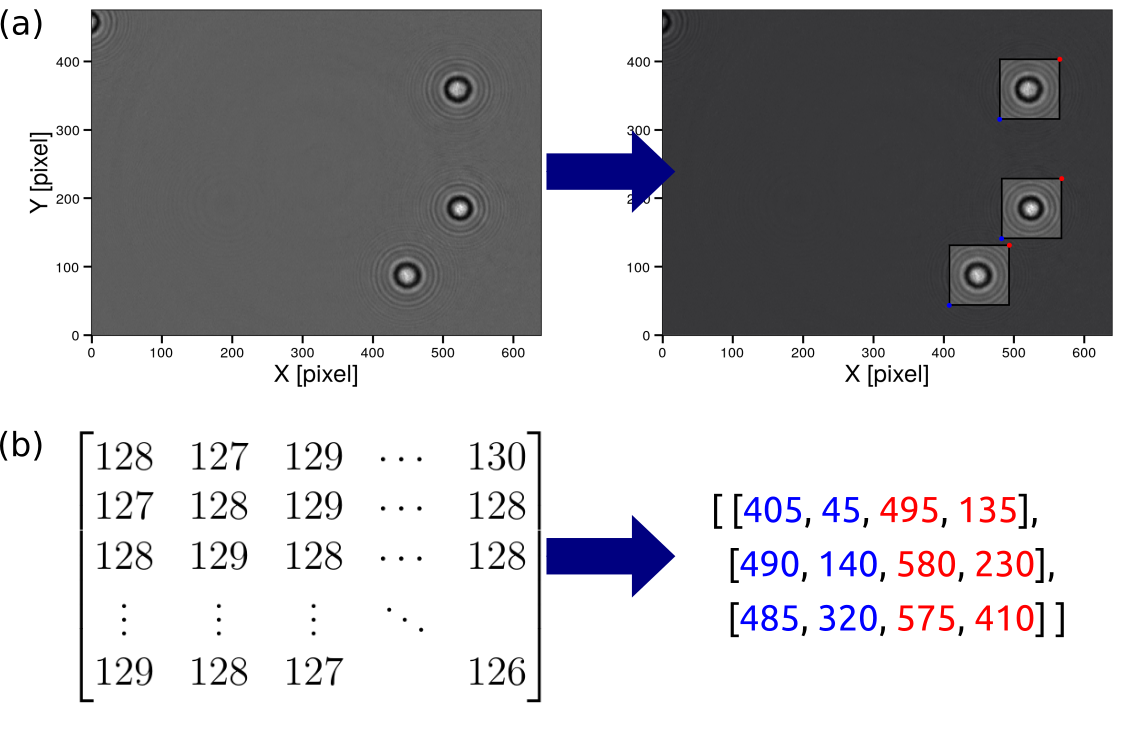
\includegraphics[width=\textwidth]{cascade_detection_FINAL}	
  \caption{ Feature detection and localization in holograms of colloidal particles.
    The holographic microscopy image includes three features due to light scattering by
    colloidal spheres in the imaging volume. All three features are detected and bounding
    boxes are placed over the region of interest around each holographic feature.
    Blue and red dots indicate the lower left and upper right corners of the feature,
    respectively. (b) Although feature
    detection seems straightforward by visual inspection, it is a more challenging
  task when posed as a purely mathematical problem.} 
  \label{fig:detection}
\end{figure}

\section{Detecting and localizing holographic features}

Figure~\ref{fig:detection}(a) illustrates the challenge of
recognizing features in holographic images: for each
feature in a video frame, the goal is to return the set of coordinates
that define a bounding box enclosing the feature.
Features may vary in contrast and in extent.
Additionally, they may overlap or be occluded by the edge of the field of view.
Figure~\ref{fig:detection}(b) conveys the computational
difficulty of automating this task. The intensity values
for each pixel in the recorded video frame are stored in a two-dimensional
array. A successful analysis of the
array yields a list whose length corresponds to the number of features and whose
entries identify the coordinates bounding a particular feature.
  
\subsection{Heuristic algorithms}
\label{sec:heuristic}

One practical method for detecting holographic features and 
locating their centers involves transforming extended interference
patterns into compact peaks \cite{cheong09,krishnatreya14a}, and 
then locating the peaks with standard centroid detectors 
\cite{crocker96,allan16trackpy}. 
Successful implementations of this two-step
approach have been based on
voting algorithms such as the circular Hough transform
\cite{cheong09,parthasarathy12,allan16trackpy} and
the orientation alignment transform \cite{krishnatreya14a}.
Both of these feature-coalescence algorithms rely on the
radial symmetry of typical single-particle holograms
without reference to the underlying image-formation
mechanism.
For an image of $N$ pixels on a side, voting algorithms
have a computational complexity of $\mathcal{O}\left (N^3 \log N \right )$ 
\cite{hollitt13} whereas the convolution-based orientation alignment
transform
runs in $\mathcal{O}\left ( N^2 \log N \right )$ operations \cite{cheong09}.
For this reason, we transform holograms with the
orientation alignment transform
to assess the performance of heuristic algorithms,
using an open-source implementation described
in \cite{cheong09}.

The peaks created by feature coalescence can be detected
and their centroids localized as local maxima in the transformed images.
We use the open-source
TrackPy implementation \cite{allan16trackpy}
of the Crocker-Grier algorithm \cite{crocker96} for this step.
When presented with holograms of well-separated
colloidal spheres, heuristic algorithms provide
sub-pixel precision for particle localization
\cite{cheong09,krishnatreya14a}.
This easily meets the need to localize
features for subsequent analysis.

Detecting and localizing local maxima can be very
efficient if the peaks have well-defined widths,
heights and separations \cite{crocker96,allan16trackpy}.
Transformed holograms of colloidal particles, however,
can have widely varying contrasts
and extents depending on the particles' properties and
heights above the focal plane.
Thresholds for feature detection and localization therefore
must be assessed from the transformed images
themselves.
This can create a bottleneck
for
heuristic feature detection and localization.

\subsection{Machine-learning algorithms}

Machine-learning techniques can reduce the computational
burden of detecting and localizing features of interest in
holographic microscopy images, and also prove to be more
robust against false positive and negative feature detections
than heuristic algorithms.
We have implemented two such approaches:
a cascade of boosted classifiers based on Haar-like wavelets,
and a deep convolutional neural network (CNN).
Both approaches yield estimates for the in-plane
coordinates, $(x_p, y_p)$, for every particle in the field
of view, as well as the extent of the region of interest
encompassing the scattering pattern.
The boxes superimposed on the two-particle hologram in
Fig.~\ref{fig:detection}(a) represent
regions of interest centered on the particles
that were computed by a CNN.

Cascade classifiers and convolutional neural networks
both work by convolving holograms with
small arrays and interpreting the results.
They thus require $\mathcal{O}\left ( N^2 \right )$ operations, which 
gives them the potential to run significantly more
quickly than heuristic algorithms, particularly for
larger images.
Each has particular strengths for particle localization
in holographic microscopy images.

Cascade classifiers were originally developed for detecting 
faces in photographs \cite{viola2001rapid}. 
They work by convolving an image with a sequence of 
selected wavelets, each of which is considered to be a
``weak classifier'' for objects of interest.
An above-threshold response from a linear combination of such
weak classifiers signifies the presence of a feature
centered at the point of strongest response.
Regions containing such above-threshold responses are analyzed
with the weak classifiers at the next step of the cascade.
Any regions that remain after analysis by the full cascade are
considered to be features.
The analysis is performed at a sequence of resolutions to capture
features at different scales.
Haar wavelets are particularly attractive
for this application because they are implemented in
integer arithmetic with highly efficient algorithms.
The training process determines
which Haar wavelets constitute useful weak classifiers
at each level of the cascade, and which combinations best
serve as strong classifiers.
Training also optimizes the number of stages of increasingly
fine resolution required to detect features reliably and to
localize them with a specified precision.
This approach has been adapted for a wide range of
object recognition and image segmentation tasks
\cite{lienhart2002extended}.
Our application of this technique to holographic feature 
localization is based on an open-source implementation
of Haar cascade classifiers made 
available by the OpenCV project \cite{itseez2015opencv}.
This cascade classifier can be trained to recognize non-standard
features of interest, such as holograms of colloidal particles.
For each such feature in a hologram, it yields
a candidate set of rectangular regions of interest that
may include multiple estimates for each feature.
Overlapping detections can be coalesced with
standard algorithms for non-maximum suppression
\cite{neubeck06}.
The center of each resulting rectangle constitutes an
estimate for the associated feature's position in the focal plane.

Convolutional neural networks also solve image recognition
tasks through convolutions with selected kernels. In this case,
the convolutions are integrated into the network's
multi-layered, feed-forward architecture 
\cite{sermanet2013overfeat} and employ kernels that are designed
and optimized during training.
Constructing a CNN to perform general image classification 
requires massive computational resources \cite{tensorflow2015-whitepaper}.
Once constructed, however, a CNN can be
retrained easily to recognize particular features of interest.
Our application of CNNs for feature localization is based on 
TensorBox \cite{stewart2015endtoend}, an open-source package 
built on the GoogLeNet-OverFeat network \cite{sermanet2013overfeat},
specifically on Inception v1 \cite{szegedy15}.
Tensorbox provides a convenient interface for training the
input layers of Inception to recognize holograms of spheres
and the for training the output layers to associate these features
with regression estimates for the
locations and extents of detected features.

\begin{figure}[b!]
  \centering
  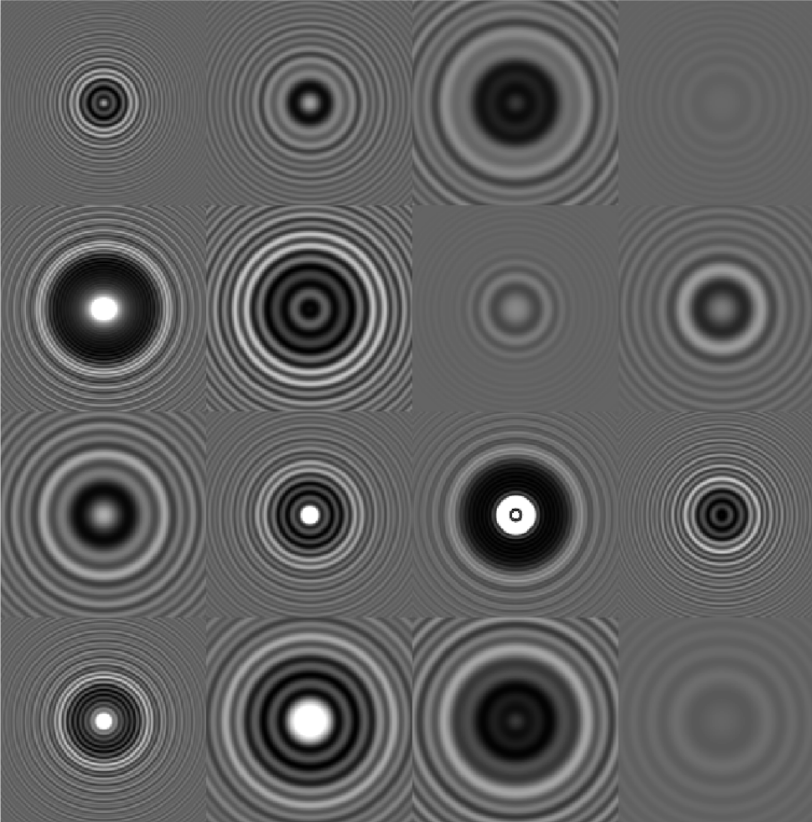
\includegraphics[width=\textwidth]{rogue_gallery}	
  \caption{ A random selection of synthetic
  holographic features used to train machine-learning algorithms.} 
  \label{fig:rogue_gallery}
\end{figure}

Both types of supervised machine-learning algorithms 
require sets of sample data for training and validation.
Each training element
consists of an image containing
zero, one or more features together with
a ``ground truth'' annotation for each feature in that image
specifying the features' locations and extents.
Standard practice involves obtaining images experimentally
and annotating them by hand.
We instead train with synthetic holograms that are 
computed with the same light scattering theory \cite{lee07a}
used to analyze experimental holograms.
Using the physics of image formation
for the ground truth for training eliminates 
the effort and errors inherent in empirical annotation and is
one of the original contributions of this work.

\section{Generating training and validation datasets}

We use Eqs.~\eqref{eq:gen_norm} through \eqref{eq:bn} to generate training 
images of spherical scatters with radii ranging from 
$a_p = \SI{0.25}{\um}$ to \SI{5}{\um}, refractive indexes from 
$n_p = \num{1.4}$ to \num{2.5}, and axial positions from 
$z_p = \SI{5}{\um}$ to \SI{50}{\um}. 
Each training hologram has parameters selected at 
random from this 
range and is centered at random within
the field of view.
Normalized experimental holograms have uncorrelated white
noise that we model as additive Gaussian noise with a standard
deviation of five percent. Figure~\ref{fig:rogue_gallery} depicts
\num{16} randomly selected, cropped, and centered synthetic features
used in training.

Our cascade classifier was trained with \num{6000}
synthetic images of colloidal spheres.
These were combined with a complementary set of 
\num{4000} particle-free images recorded by the instrument itself.
Each computed image is annotated with
the coordinates of the corners defining that feature's region of
interest.
The region is centered on the feature's actual position
and has an extent that encloses 10 interference fringes.
The classifier was trained
until its rate of false positive detections
fell to \num{8E-4}.
This was achieved with a classifier that searches for features
through five resolution stages, with each stage being
comprised of a distinct set of five wavelets.
This geometry and the choice of weak classifiers was arrived at
by the training algorithm's optimizer.

The convolutional neural network was trained with 
\num{3000} synthetic holographic images; another \num{600} 
were used for validation.
These images also were annotated with feature positions and extents
drawn from the ground truth for the image-formation process.
CNN training converged after \num{50000} cycles
of training and validation.

\subsection{Precision and accuracy}
  
\begin{figure}[!t]
  \centering
  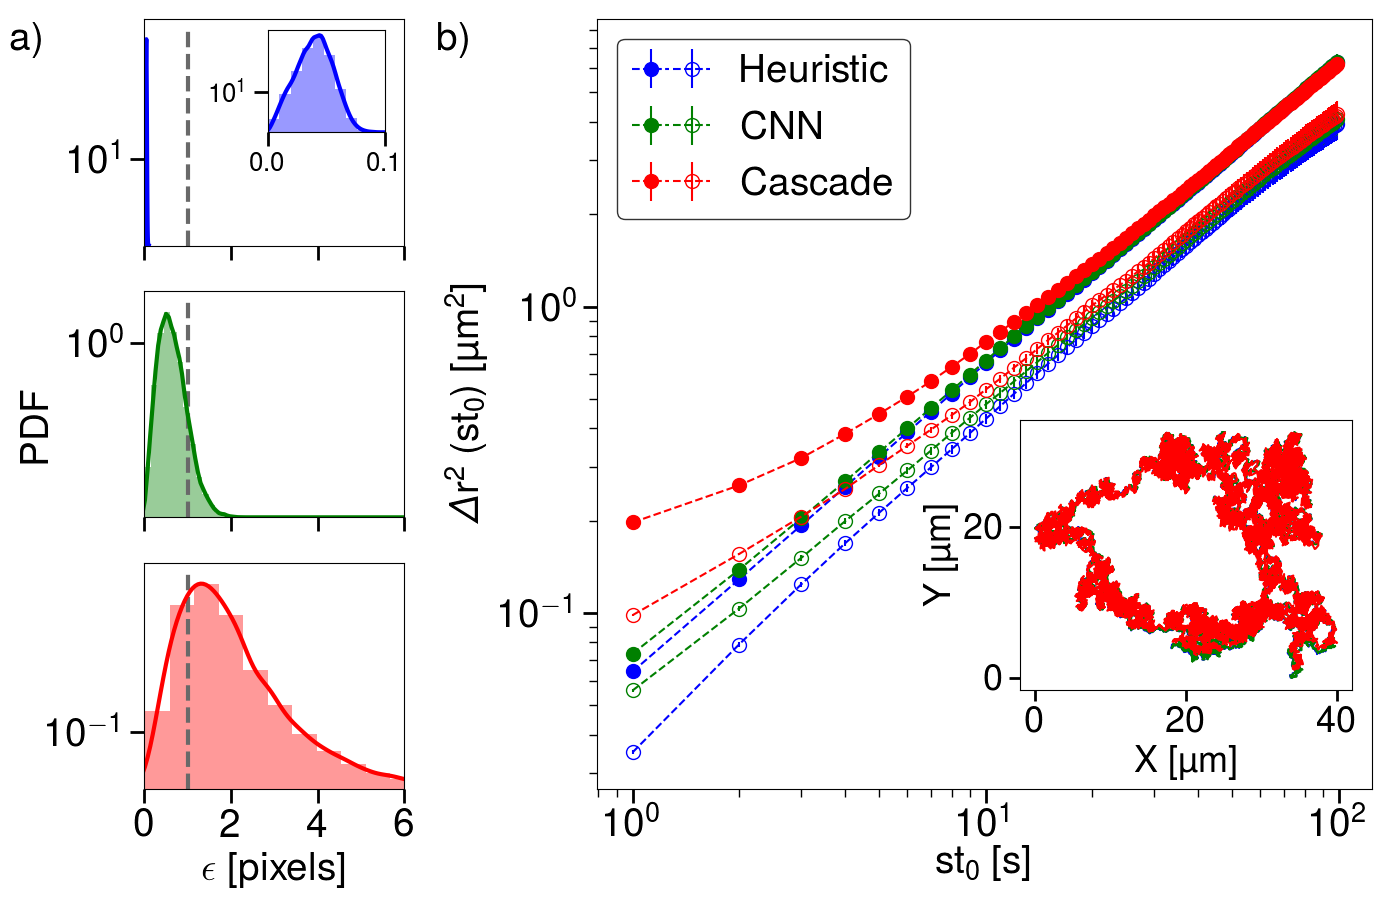
\includegraphics[width=\columnwidth]{cascade_02} % FIXME CHECK that this
  %is the figure david used.
  \caption{Estimating the simulated trajectory of a Brownian particle.
  (a) Probability distribution functions for the
  localization error achieved by (top) heuristic
  algorithm, (middle) convolutional neural network,
  and (bottom) cascade classifier. 
  The inset in the top panel shows an expanded view of the heuristic algorithm's subpixel
  resolution. Vertical dashed line indicates single-pixel
  precision.
  (b) Mean-square displacement computed from 
  trajectories obtained with the three detection algorithms.
  Short-time asymptotes yield dynamical estimates
  for the localization error.
  Open circles represent experimental data,
  as explained in Sec.~\ref{sec:experiment}\cite{hannel18}.
  }
  \label{fig:msdplot}
\end{figure}

\begin{figure}
  \centering
  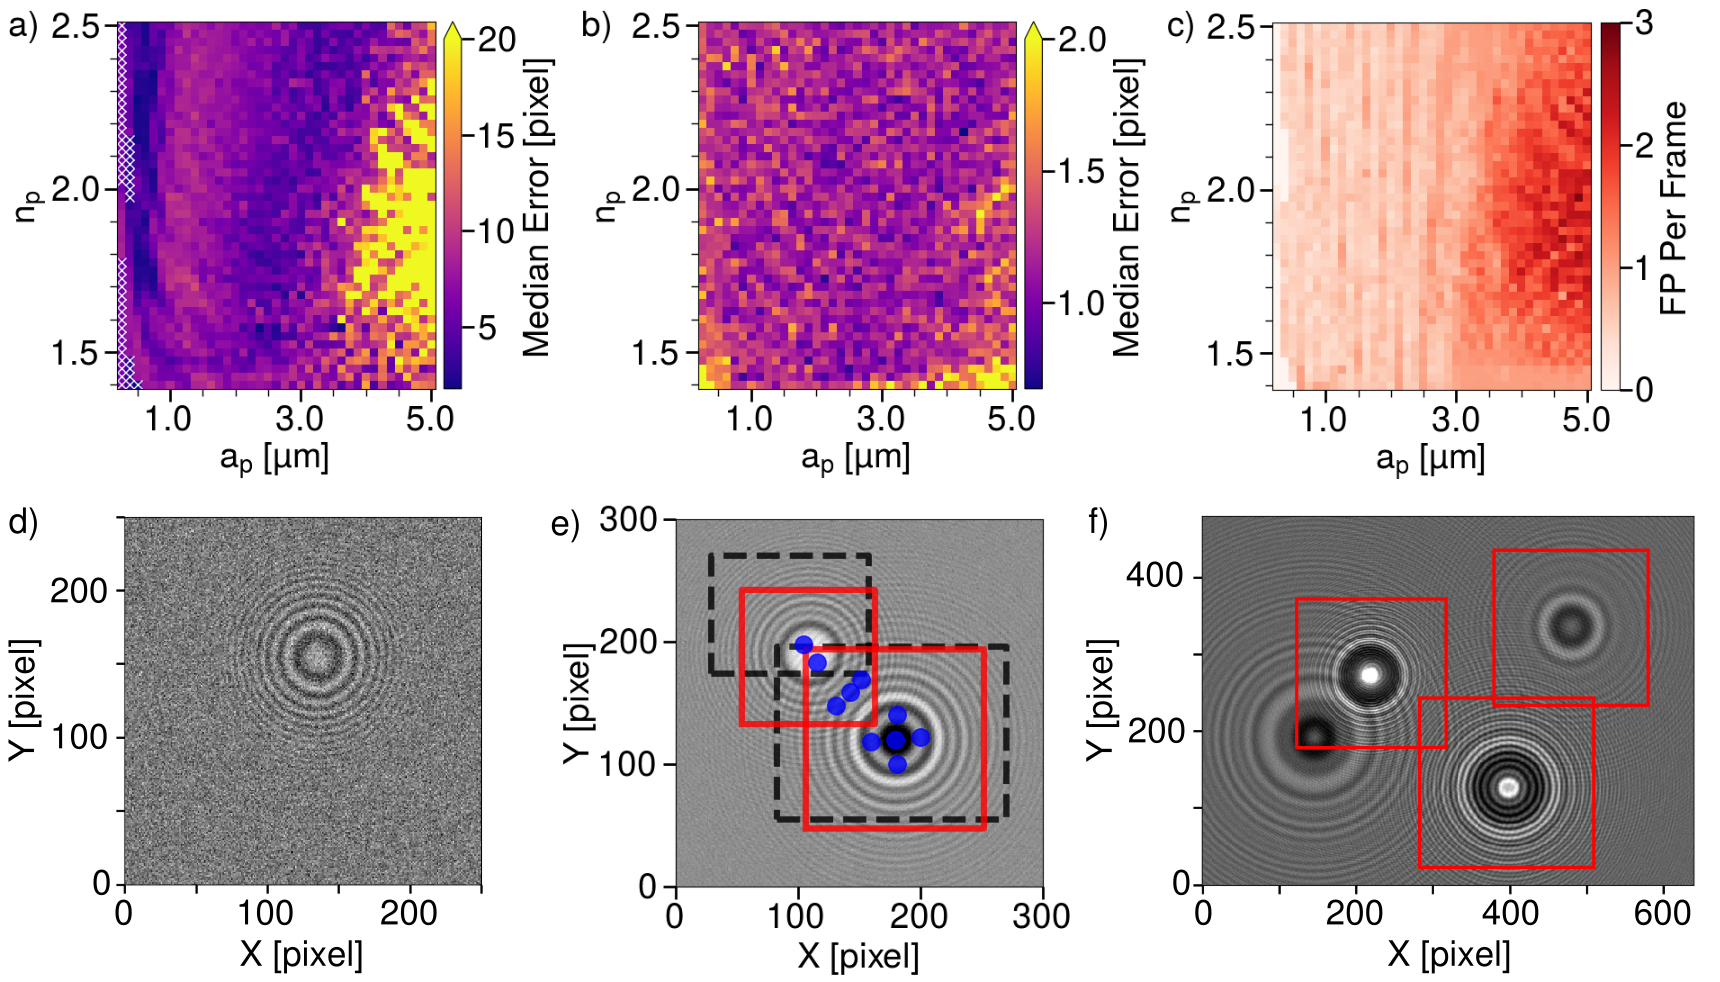
\includegraphics[width=\textwidth]{cascade_03}
  \caption{Localization errors as a function of particle
  radius and refractive index at a height of $z_p = \SI{13.5}{\um}$
  above the focal plane as obtained with (a) the cascade classifier,
  and (b) the convolutional neural network.
  (c) Rate of false positive detections reported by the 
  cascade classifier. (d) Hologram of a \SI{500}{\nm}-diameter silica sphere that was
  overlooked by the cascade classifier.  This particle was localized
  to within one pixel by the CNN.
  (e) Hologram of a \SI{2.4}{\um}-diameter
  polystyrene sphere (upper left) interfering with the hologram of
  a \SI{4.0}{\um}-diameter TPM sphere located \SI{15}{\um} above it.
  Blue dots show feature locations proposed by the heuristic
  algorithm; Red boxes enclose features detected by the CNN; 
  Dashed black boxes are proposed by the cascade classifier.
  (f) Hologram of four particles
  overlaid with regions of interest identified by the CNN.  One
  occluded feature was overlooked by the CNN\cite{hannel18}.
  }
  \label{fig:figure3}
\end{figure}

We assess the detectors' localization precision by 
comparing detection results with known 
input parameters.
A typical example for a particular choice of particle
properties is shown in Fig.~\ref{fig:msdplot}.
The three probability distributions 
in Fig.~\ref{fig:msdplot}(a) present
the root-mean-square localization error
obtained by each of the algorithms when tracking
particles with
$a_p =\SI{1.0}{\um}$ and $n_p = \num{1.5}$.
We generate data for these plots by simulating the
diffusion of such a particle through water
at a temperature of \SI{20}{\celsius} starting from 
the center of the field of view at $z_p=\SI{13.5}{\um}$
and proceeding for \num{3000} steps at \SI{33}{\ms} per step.

The heuristic algorithm consistently 
yields sub-pixel precision with a median error of 
\SI{0.04}{pixels}. 
The convolutional neural network also yields sub-pixel
precision with a median localization error of \SI{0.61}{pixels}.
The cascade classifier performs less well,
with a median localization error of \SI{1.81}{pixels} and
a substantial probability
for errors extending to several pixels.
For applications such as Lorenz-Mie microscopy
that require input estimates with sub-pixel precision,
the cascade classifier's localization precision may not
be sufficient.

The inset of Fig.~\ref{fig:msdplot}(b) shows the trajectory
reconstructed by each of the algorithms.
The measured trajectory's mean-squared displacement (MSD)
provides an estimate for the particle's
diffusion coefficient.
All three methods yield results that are consistent with
the particle's true diffusivity,
$D = \SI{0.482}{\um^2 \per \second}$,
which suggests that
their localization errors are normally distributed.
Extrapolating the MSD to zero lag time 
provides an estimate for the localization error \cite{crocker96,michalet12}.
In all three cases, the extrapolated measurement error
is consistent with the median values from Fig.~\ref{fig:msdplot}(a). 

Applying the same techniques across the entire range of particle
sizes and refractive indexes yields results for the median
localization error summarized in
Figs.~\ref{fig:figure3}(a) and \ref{fig:figure3}(b).
Results from the cascade classifier in Fig.~\ref{fig:figure3}(a)
range from single-pixel precision under most conditions to 
more than 20 pixels for the largest spheres we considered.
These errors are dominated by the cascade classifier's tendency
to displace location estimates toward the center of the
field of view when presented with features that extend outside
the observation window.
This problem is more pronounced
for the larger holographic features created by larger scatterers.
Smaller particles create holograms with low signal-to-noise 
ratio that can be overlooked by the cascade classifier leading
to false negative detections.
Such conditions are indicated by white crosses in
Fig.~\ref{fig:figure3}(a).
A typical example of such a challenging hologram is
shown in Fig.~\ref{fig:figure3}(d).

The results plotted in Fig.~\ref{fig:figure3}(b) show that
the CNN yields much smaller
localization errors than the cascade classifier.
The CNN achieves sub-pixel
resolution over the entire range of parameters,
although localization precision is worse for
weak scatterers and large spheres.
Unlike the cascade classifier, it returned no
false negative results, and even achieved single-pixel
precision for the low-contrast hologram in
Fig.~\ref{fig:figure3}(d) \cite{hannel18}.

Both the cascade classifier and the CNN
return a small rate of false positive detections.
Figure~\ref{fig:figure3}(c) reports the false-positive
rate for the cascade classifier, which ranges from
\SI{E-1}{frame^{-1}} for holograms of particles with
$a_p < \SI{3}{\um}$
to \SI{3}{frame^{-1}} for holograms of larger spheres.
In all cases, these false positive detections come in addition
to the correct particle detection, and result from
the classifier's failure to correctly coalesce multiple detections
of the same particle.
Such false positive detections contribute to the very large
localization error for large spheres in Fig.~\ref{fig:figure3}(a).
The CNN performs substantially
better, with fewer than one false positive per thousand
frames.

\subsection{Multiple particles}

The results presented so far apply to holograms of single
particles.
In practice, it is not unusual for multiple particles to enter 
the microscope's field of view simultaneously.
Their scattering patterns interfere to create
intensity variations that can confuse heuristic detection algorithms.
Depending on the particles' proximity and alignment, their
holograms can merge into irregular patterns whose analysis
requires more specialized techniques \cite{perry12,fung13}.
The hologram in Fig.~\ref{fig:figure3}(e)
illustrates the effect of more modest overlap.
It captures a \SI{2.4}{\um}-diameter
polystyrene sphere \SI{17}{\um} above the focal plane
whose hologram is partially occluded by that 
of a \SI{4.0}{\um}-diameter TPM sphere situated \SI{15}{\um}
above and \SI{15}{\um} off to the side.
Discrete points overlaid on this image show the
positions that the heuristic algorithm
identified as centers of candidate features.
Of the 10 proposed features, 8 are false positive detections
and one correct localization is poorly localized.

Both machine-learning algorithms perform better than the
heuristic algorithm for this image.
The cascade classifier correctly
detects both particles, as indicated by dashed rectangles
in Fig.~\ref{fig:figure3}(d).
The estimated locations, however, are displaced significantly
from the features' true centers, presumably because of
interference between the two scattering patterns.
The CNN not only detects and localizes
both particles correctly, but also provides useful estimates for the
extent of the scattering patterns, as denoted by the solid (red)
squares overlaid on Fig.~\ref{fig:figure3}(d).

More substantial overlap can confound the CNN,
leading to false-negative detections.
Figure~\ref{fig:figure3}(f) shows a hologram with
overlapping features due to four spheres
located in four different planes over a \SI{50}{\um} axial
range.
The CNN correctly detects and
localizes three particles, and provides reasonable
estimates for their features' extents.
The fourth feature, which is larger and has lower contrast,
is omitted.
Such false negatives become more common as the number and
extent of features in a hologram increases.
Standard bright-field imaging would miss even
more of these particles because the axial range
over which they are distributed greatly exceeds
a conventional microscope's depth of focus.

These results illustrate that machine-learning algorithms can
be more reliable than heuristic algorithms for detecting and
localizing features in non-ideal holograms.
For applications such as monitoring colloidal concentrations, this
benefit alone might recommend machine-learning algorithms
over other approaches.
The principal benefit of machine-learning algorithms, however,
is their ability to detect features rapidly, even on
low-power computational platforms.

\subsection{Computation speed}

\begin{table}[b!]
\centering
\caption{Analysis times in ms/frame for the heuristic
  algorithm, the convolutional neural network (CNN) implemented on
  CPU and GPU, and the cascade classifier implemented on a
  workstation and on a Raspberry Pi 3 single-board computer\cite{hannel18}.}
\begin{tabular}{lrrrrr}
\hline
\hline
  & \text{Mean~[ms]} & \text{Median~[ms]} & \text{Std.~[ms]} &
                                                               \text{Min~[ms]} & \text{Max~[ms]} \\
Heuristic (CPU) & 695 & 700 & 11 & 670 & 1000 \\ 
CNN (CPU) & 278 & 278 & 2.8 & 271 & 315 \\
CNN (GPU) & 52 & 52 & 4.8 & 50 & 70 \\
Cascade (CPU) & 17 & 17 & 1.0 & 15 & 81 \\ 
Cascade (RPi) & 173 & 171 & 12 & 159 & 275 \\ \hline \hline
\end{tabular}
\label{table:times}
\end{table}

Table~\ref{table:times} presents timing data for holographic
feature detection on a \SI{1}{Gflops} desktop workstation
outfitted with an
nVidia GTX 680 GPU.
This system can detect a single feature in just under
\SI{700}{\ms} using the heuristic
algorithm described in Sec.~\ref{sec:heuristic}.
Of this, \SI{150}{\ms} is required for the orientation alignment
transform and half a second is required to analyze the
transformed image and then to detect and localize
its peaks.
This bottleneck can be reduced to \SI{50}{\ms} by specifying
the anticipated width, height and separation of the
transformed peaks.
In this case, the present implementation's processing speed
is consistent with previous reports \cite{lee07a,cheong09,allan16trackpy}
when account is taken of image size and processor speed.
No single set of such parameters, however, successfully detects
features over the entire range of parameters considered in
Fig.~\ref{fig:figure3}.
The slow operation reported in Table~\ref{table:times}
therefore represents the cost of generality.

The CNN routinely
outperforms the heuristic algorithm by
a factor of \num{2.5} on the same hardware over the entire
range of parameters.
Transferring the CNN calculation to the GPU
increases this advantage to a factor of \num{11}.
Most remarkably, the cascade classifier is \num{40} times
faster than the reference heuristic algorithms,
even without GPU acceleration, processing features
fast enough to keep up with the \SI{33}{\ms} frame
rate of a standard video camera.

The cascade classifier is so computationally efficient
that it can be deployed usefully on a lightweight
embedded computer. 
We demonstrate this by analyzing holograms on
a Raspberry Pi 3 single-board computer.
Even though the light-weight computer runs the
cascade classifier \num{10} times slower than the
workstation,  it is still \num{4} times faster than the heuristic 
algorithms on the workstation.
Reducing the resolution by half, improves the 
Raspberry Pi's detection time to \SI{40}{\ms} per image 
which corresponds to \SI{25}{frames \per \second}.

\subsection{Experimental demonstrations}
\label{sec:experiment}

\begin{figure}[!b]
  \centering
  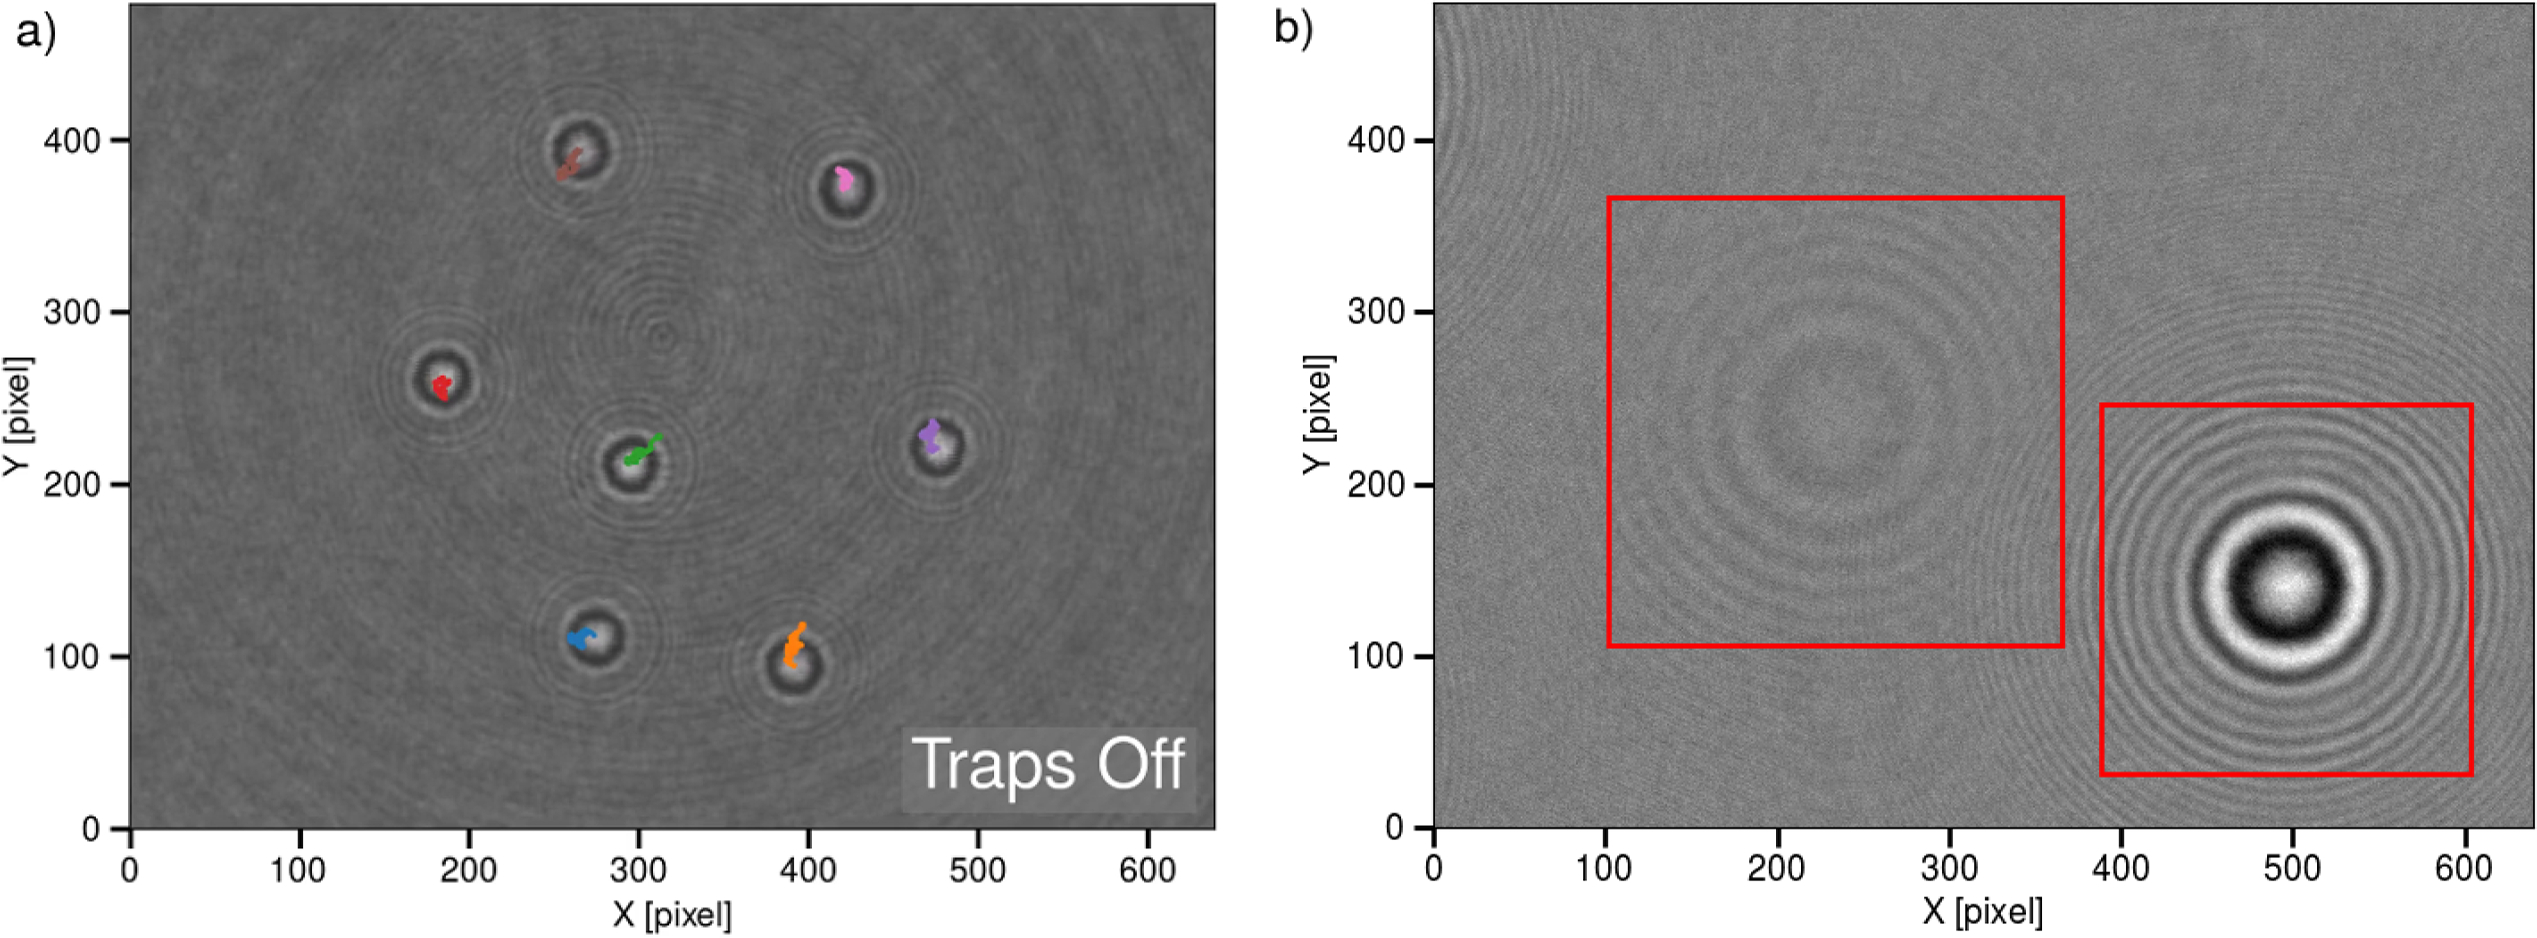
\includegraphics[width=\textwidth]{cascade_04}
  \caption{(a) Cascade classifier tracking \SI{2}{\um}-diameter
    colloidal spheres diffusing through water in a
    holographic optical trapping system.
    Each trace shows 5 seconds of the associated particle's motion.
    These tracking data were used successfully to trap
    the particles.
    (b) CNN detection of holographic features.
    The high-contrast feature is created by a \SI{1.5}{\um}
    diameter silica sphere.  The low-contrast feature
    represents a coliform bacterium in the dispersion \cite{hannel18}.}
  \label{fig:autotrap}
\end{figure}

Real-time detection of holographic features has applications
beyond holographic particle characterization.
The implementations presented here are suitable for targeting
optical traps in holographic trapping systems \cite{grier03}.
We have demonstrated this by integrating machine-learning
particle detection into an automated trapping system that
projects optical traps onto the particles' positions to acquire
them for subsequent processing.
Pioneering implementations
of automated trapping \cite{chapin06} rely on conventional
imaging and so require target particles to lie near the microscope's
focal plane.
Holographic targeting works over a much larger axial
range.
Both the CNN and the cascade classifier
locate particles in the plane with sufficient precision to ensure
reliable trapping.
The axial coordinate required for three-dimensional targeting can
be extracted from holographic features using previously reported
techniques \cite{yevick14}.
Because of its speed, the cascade classifier is particularly useful
for targeting fast-moving particles.
Figure~\ref{fig:autotrap}(a) shows the cascade classifier tracking colloidal
particles in real time as they diffuse in a holographic trapping
system.
Position estimates are good enough that holographic traps guided by the
cascade classifier routinely trap all of particles in the field of view.

Figure~\ref{fig:autotrap}(b) shows typical results obtained with
the CNN analyzing experimental data.  The image
is a normalized hologram of a
\SI{1.5}{\um}-diameter silica sphere dispersed in water
flowing down a \SI{100}{\um}-deep microfluidic channel.
The second holographic feature in this image is due
to a coliform bacterium in the sample \cite{philips17}.
The CNN detects and correctly localizes
both features despite their substantial
difference in contrast.

We can estimate the feature-detection algorithms' precision
for particle localization by tracking diffusing particles
\cite{crocker96}.
The open circles in Fig.~\ref{fig:msdplot}(b) show results obtained
with heuristic and machine-learning algorithms for the
mean-square displacement of a single colloidal polystyrene sphere
(Duke Scientific, catalog no.\ 4016A, nominal diameter
\SI{1.587+-0.018}{\um}) diffusing through water at
room temperature.
Because polystyrene is \SI{5}{\percent} more dense than water,
the particle sediments \SI{11}{\um} over the course of this
\SI{3}{\minute} measurement.
In all three cases, the in-plane localization error obtained
by extrapolating these results is consistent with that
reported for synthetic data.

\section{Discussion}

Using machine-learning algorithms to detect and
localize holographic features enables and enhances a host of 
applications for holographic video microscopy.
CNNs detect and localize colloidal
particles faster than conventional image-analysis techniques
and localize particles well enough for subsequent processing.
Our implementation also estimates the extent of each holographic feature 
thereby bypassing the standard next step in Lorenz-Mie microscopy
\cite{cheong09} and saving additional time.
These substantial speed enhancements make it possible to
perform holographic particle characterization measurements in real
time rather than requiring off-line processing.
CNNs also are more successful at
interpreting overlapping features in multi-particle
holograms and thus can be used to analyze more concentrated
suspensions.

The Haar-based cascade classifier also outstrips the heuristic algorithms'
ability to detect colloidal particles, particularly in heterogeneous
samples and crowded fields of view.
Although it cannot match the localization precision of CNNs,
its speed and modest computational requirements
create new opportunities.
We have deployed our cascade classifier on a light-weight
single-board computer and have demonstrated its utility for counting particles
and thus for measuring colloidal concentrations.
Such a low-cost instrument should be useful for routine monitoring of
industrial processes and products and for environmental monitoring.
We also have demonstrated the cascade classifier's utility for
high-speed targeting in holographic trapping.  In this case, speed
is more important than localization precision for interacting with
processes as they unfold.

While the present study focuses on detecting and localizing
holographic features with radial symmetry,
the machine-learning framework can be applied equally well to
asymmetric holograms produced by rods, clusters
or biological samples.
By reducing the computational burden of analyzing holograms,
machine-learning algorithms extend the reach of holographic
tracking and holographic characterization.
More generally, machine-learning algorithms are well-suited to bootstrapping
the more detailed analysis involved in holographic particle
characterization.
We anticipate that more of these physics-based
processing steps will be taken over by machine-learning algorithms
as that technology advances.

This work was supported primarily by the MRSEC program of the
National Science Foundation through Award Number DMR-1420073
and in part by the SBIR program of the NSF through Award Number
IPP-1519057.
The holographic trapping instrument was developed under the
MRI program of the NSF through Grant Number DMR-0922680.

    \newpage
    
    \chapter{Machine-learning approach to holographic particle characterization}
\label{ch:svr}

\section{Introduction}

The previous chapters establish that holograms of colloidal spheres obtained 
with holographic video microscopy
\cite{sheng06,lee07}
can be interpreted with predictions of the Lorenz-Mie theory 
of light scattering \cite{bohren83}
to track each particle in three dimensions, and to measure 
its size and refractive index \cite{lee07a}.
State-of-the-art implementations \cite{lee07a,bourquard13,seifi13,fung13}
can locate a sphere and resolve its
radius both to within a few nanometers, and 
can determine its refractive index to within a part per thousand
\cite{cheong09,shpaisman12,krishnatreya14}.
The cost of this powerful technique is the computational burden of
either fitting each hologram pixel-by-pixel to theoretical predictions
\cite{lee07a,cheong10a} or performing a Bayesian inference of the
model parameters \cite{dimiduk16}.
Here, we demonstrate that techniques of machine learning
can reduce the processing time by a factor of a thousand,
yielding real-time performance.

This chapter describes an approach to fast holographic characterization,
depicted schematically in Fig.~\ref{fig:method}, that
employs the support vector machine (SVM) algorithm
\cite{smola04} 
to compare experimental measurements with
pre-computed predictions of the Lorenz-Mie theory
\cite{bohren83,lee07a,krishnatreya14a}.
Whereas nonlinear fitting typically requires more than a second
on a \SI{1}{\giga flop} computer,
a trained SVM can estimate the size, refractive index or
axial position of a micrometer-scale sphere
in under a millisecond on the same hardware.

\begin{figure}
  \centering
  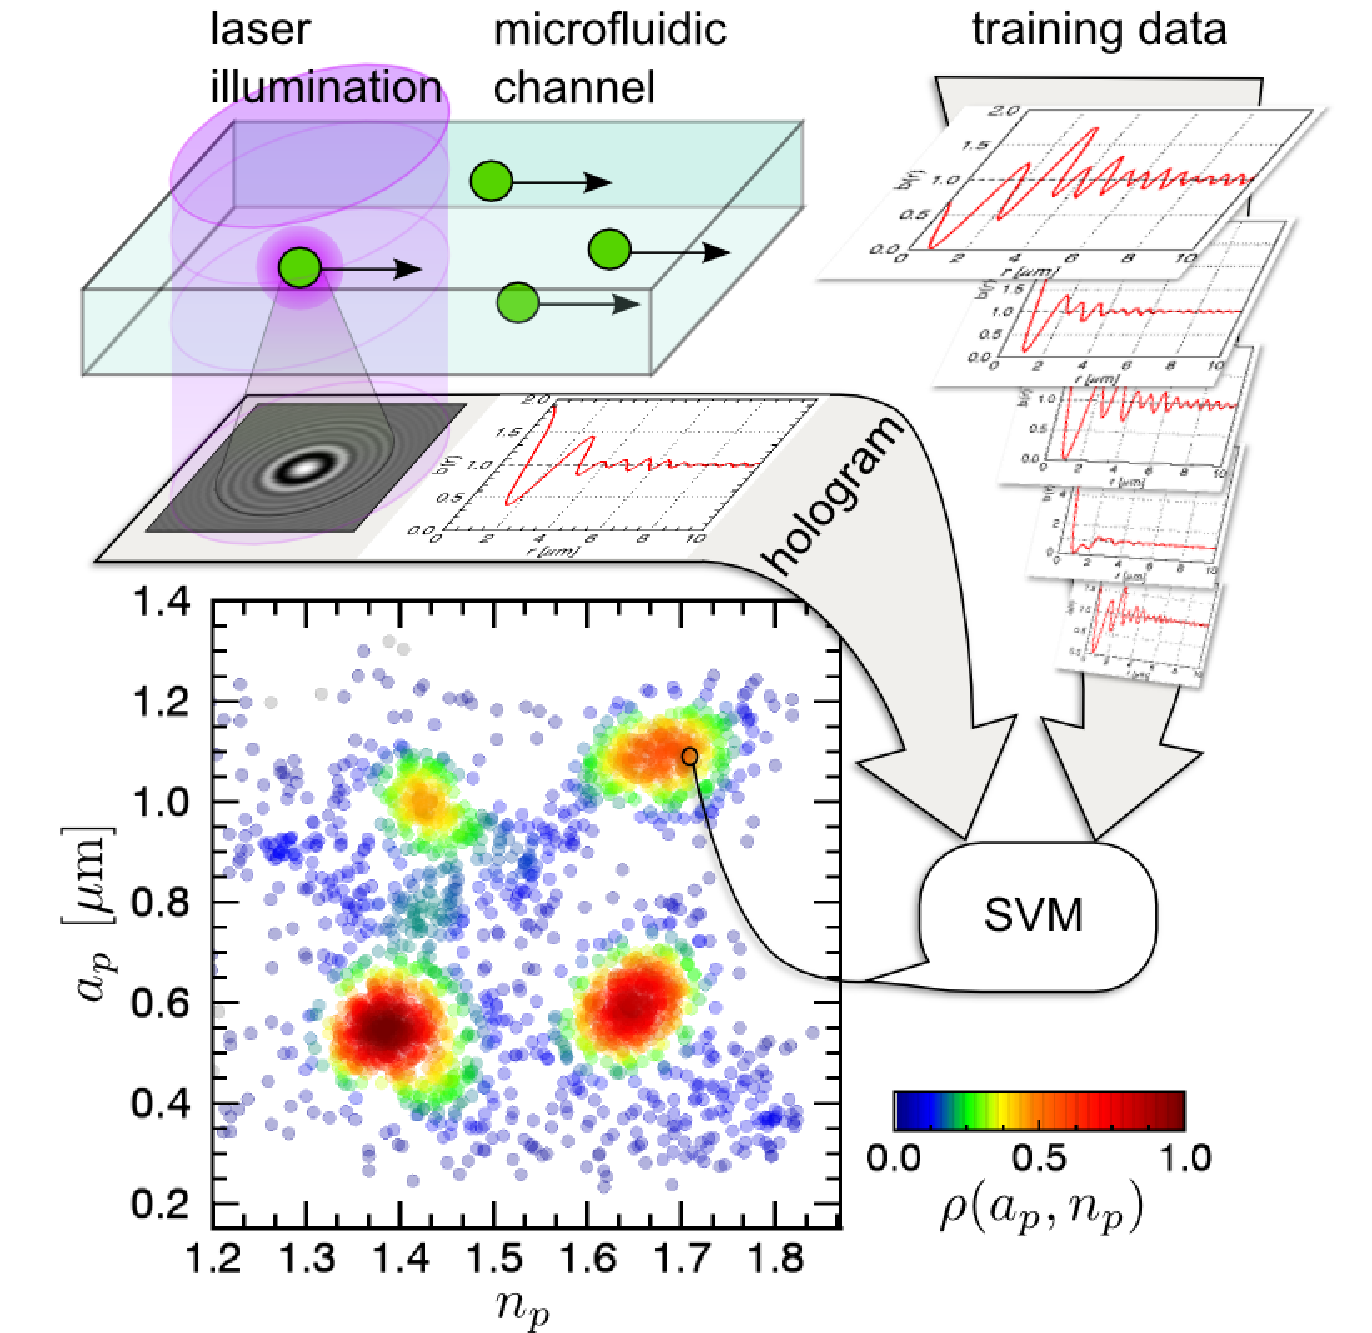
\includegraphics[width=\textwidth]{svr_figure1}
  \caption{Colloidal characterization by holographic microscopy and
    machine learning.  Colloidal spheres flowing down a microfluidic
    sample scatter light from a collimated laser beam to form an
    in-line hologram.  Features in the beam are identified, and their
    radial profiles are presented to support vector machines (SVMs)
    that compare them with a library of training data to estimate
    each spheres' radius $a_p$ and refractive index
    $n_p$.  The scatter plot shows results for 2,500 spheres
    drawn at random from a mixture of four different types of
    spheres.  Each point is colored by the local density of
    data points, $\rho(a_p,n_p)$ \cite{yevick14}.}
  \label{fig:method}
\end{figure}

\section{Fast Holographic Characterization with Machine Learning}

Previous implementations of Lorenz-Mie microscopy \cite{lee07a} 
fit Eqs.~\eqref{eq:gen_norm} through \eqref{eq:bn} to measured holograms using $a_p$, $n_p$
and $\vec{r}_p$ as adjustable parameters.
These fits are exquisitely sensitive to errors in the particle's
in-plane position, and so must be performed over the entire
two-dimensional intensity distribution \cite{lee07a}.
Here, we instead use Eqs.~\eqref{eq:gen_norm} through \eqref{eq:bn} to train
support vector machines, which then are able to estimate 
$a_p$, $n_p$ and $z_p$ from a hologram's one-dimensional
radial profile.
We obtain these profiles from measured holograms by averaging
around centers of rotational symmetry \cite{krishnatreya14a}
with single-pixel resolution, yielding 100-point data vectors.
The microscope's focal plane is adjusted so that the interference
fringes in a typical sphere's hologram extend to roughly this scale.
Averaging over angles to obtain a radial profile reduces the
dimensionality of the analysis problem and accounts in
part for our method's computational efficiency.

Our SVMs are 
implemented with {\tt scikit-learn}, an open-source
machine learning software package \cite{pedregosa11} that
builds upon the {\tt libsvm} library of Support Vector Machine algorithms
\cite{chang01,chang02}.
Each SVM computes one output parameter from an input vector
consisting of a radial profile, $b(r)$, that has been digitized
into 100 single-pixel bins.
Characterizing and tracking a colloidal particle therefore requires
three SVMs, one for each of $a_p$, $n_p$ and $z_p$.
Figure~\ref{fig:method} schematically represents this process
for estimating $a_p$ and $n_p$.

An SVM computes its output by comparing
$b(r)$ with vectors from a set of training data, $\left \{ b_n(r) \right \}$,
that are computed with Eqs.~\eqref{eq:gen_norm} through ~\eqref{eq:bn} over a range
of values of $a_p$, $n_p$ and $z_p$.
Each computed profile, $b_n(r)$, constitutes one support vector in the space 
spanned by these parameters.
To facilitate these comparisons,
we construct SVMs with radial basis functions
\cite{smola04},
\begin{equation}
  \label{eq:5}
  k_n(b)
  =
  \exp\left( -\gamma \int \abs{b_n(r) - b(r)}^2 \, dr \right),
\end{equation}
that quantify the similarity of the experimental input with
the $n$-th support vector.
The sensitivity of this comparison is set by $\gamma$, with
larger values favoring more precise results at the cost of requiring
more support vectors to span the parameter space.
Given a value of $\gamma$,
the training process determines a set of weights $\omega_n$
and an offset $s_0$
such that the weighted sum, 
\begin{equation}
  \label{eq:estimate}
  \tilde{s}(b) = \sum_n \omega_n k_n(b) + s_0,
\end{equation}
constitutes an estimate for the parameter, $s(b)$, that characterizes
the input data vector, $b(r)$.
In general, errors in $\tilde{s}(b)$ depend smoothly
on $\gamma$ \cite{smola04}.

To prevent overfitting, the weights $\omega_n$ are constrained to
have magnitudes less than a maximum value, which conventionally is denoted by
$C$ \cite{smola04}.
Optimizing an SVM with larger values of $C$ improves its ability to recognize its
training data, but renders it less able to interpolate smoothly
between its support vectors when presented with novel or noisy inputs.
Some candidate support vectors may be assigned small weighting
factors in optimizing $\tilde{s}(b)$ over a corpus of training data;
these are automatically eliminated from the SVM \cite{smola04}.
The choice of $\gamma$ and $C$ thus determines which support 
vectors are included in the SVM, and their relative importance for computing the output. 
Because this process is nonlinear, optimal values are obtained by
exhaustive search over the range $0.1 \leq \gamma \leq 10$ and
$0.1 \leq C \leq 1,000$.
Statistically indistinguishable results are obtained in the present application 
for values of $\gamma$ and $C$ that vary from their optimal values by
up to fifty percent. 

We trained SVMs with a 5,000-member training set of radial profiles,
$b_n(r)$.
Parameters for these computed profiles were evenly distributed over a volume in
the three-dimensional space spanned by
$\SI{13.5}{\um} \leq z_p \leq \SI{75}{\um}$,
$\SI{0.4}{\um} \leq a_p \leq \SI{1.75}{\um}$, and
$1.4 \leq n_p \leq 1.8$ at a resolution of
\SI{1.35}{\um} in $z_p$, 
\SI{0.1}{\um} in $a_p$ and 0.1 in $n_p$.
Training time increases dramatically with 
the number of training vectors, and also with larger values of $C$ and $\gamma$.
Once trained, however, an SVM translates input data vectors into 
output parameter estimates extremely rapidly.

The quality of a trained SVM can be assessed by presenting
it with independently computed cross-validation data.
Optimal values for $C$ and $\gamma$ minimize differences
between estimated parameters and the inputs.
Using a 500-member cross-validation set, we obtained
best performance for estimating $z_p$
with $C = 100$ and $\gamma = 1$, best performance
for $n_p$ with $C = 10$ and $\gamma = 0.5$, and
best performance for $a_p$ with $C = 10$ and $\gamma = 0.6$.

Sampling the entire parameter space accessible to
holographic characterization with resolution
comparable to the precision realized with nonlinear fits
\cite{lee07a}
would require more than \num{e10} training vectors.
If, however, the system of interest is characterized by a more modest range
of parameters, then results from an initial SVM analysis
can be used to generate a comparatively small set of training data
spanning the relevant range.
This specialized training proceeds rapidly
and yields substantial improvements in precision.

\section{Characterization of Colloidal Mixtures}

The data plotted in Fig.~\ref{fig:method} are
SVM estimates for the radii and refractive indexes of 2,500 
colloidal spheres flowing down a \SI{20}{\um}-deep 
microfluidic channel formed by bonding
the edges of a glass microscope cover slip to the surface of a
glass microscope slide.
The peak flow speed of 
\SI{1}{\mm\per\second} transports  
a sphere across the field of view in no fewer than  
two video frames, ensuring that every particle in the  
flow has a chance to be analyzed.  
Anisotropic blurring due to a sphere's \SI{100}{\nm} 
motion during the camera's \SI{0.1}{\ms} exposure time  
suppresses contrast along the direction of motion, but does not  
appreciably influence the azimuthal average, $b(r)$ \cite{dixon11}.  
Spurious results arising when 
multiple spheres' interference patterns overlap
contribute outliers to the observed
distribution of particle sizes and refractive indexes.
Such artifacts are minimized by diluting the sample to a volume
fraction less than \num{e-3} so that 
no more than three particles are present in any frame.

The sample was prepared by dispersing roughly equal proportions 
of four types of colloidal spheres in water:
\SI{1}{\um}-diameter and \SI{2}{\um}-diameter 
spheres made of polystyrene (Thermoscientific Catalog No.\ 5100A and 
Bangs Laboratories Catalog No.\ SS04N, respectively) and similarly
sized spheres of silica (Duke
Standards Catalog Nos.\ 8100 and 4202A, respectively).
Each of these four populations is monodisperse, with a
standard deviation in the radius of less than 5\%.
This four-component mixture was 
flowed through the
observation volume during a \SI{12}{\minute} interval,
and analyzed particle-by-particle.
Each data point in Fig.~\ref{fig:method} corresponds to an individual 
sphere, and is colored by the local density of measurements.

SVM-mediated holographic characterization clearly identifies
the four populations of particles and provides estimates for their relative abundances.
The mode values of the refractive indexes, $n_p \approx \num{1.4}$ 
and \num{1.6}, are consistent with values for silica and polystyrene,
respectively.  Values for the radii, $a_p \approx \SI{0.5}{\um}$
and \SI{1}{\um}, are consistent with manufacturers'
specifications.
Characterizing multicomponent dispersions
is a unique capability of holographic particle analysis, and
can be performed with SVMs as fast as 
particles' holograms can be acquired.
This performance is all the more noteworthy because the
distribution of particle properties is built up one particle at a time
and so does not rely on \emph{a priori} assumptions.

Neither the instrument nor the analytical technique requires
extensive calibration.
The wavelength of the laser and the effective magnification can be
calibrated once and used for all samples.
The refractive index of the medium is the only free parameter, 
and often can be obtained separately.
These parameters are used to train the SVMs in advance,
after which they can be used to analyze arbitrary samples
dispersed in the medium.

\section{Tracking and Assessment of Precision}

\begin{figure}
  \centering
  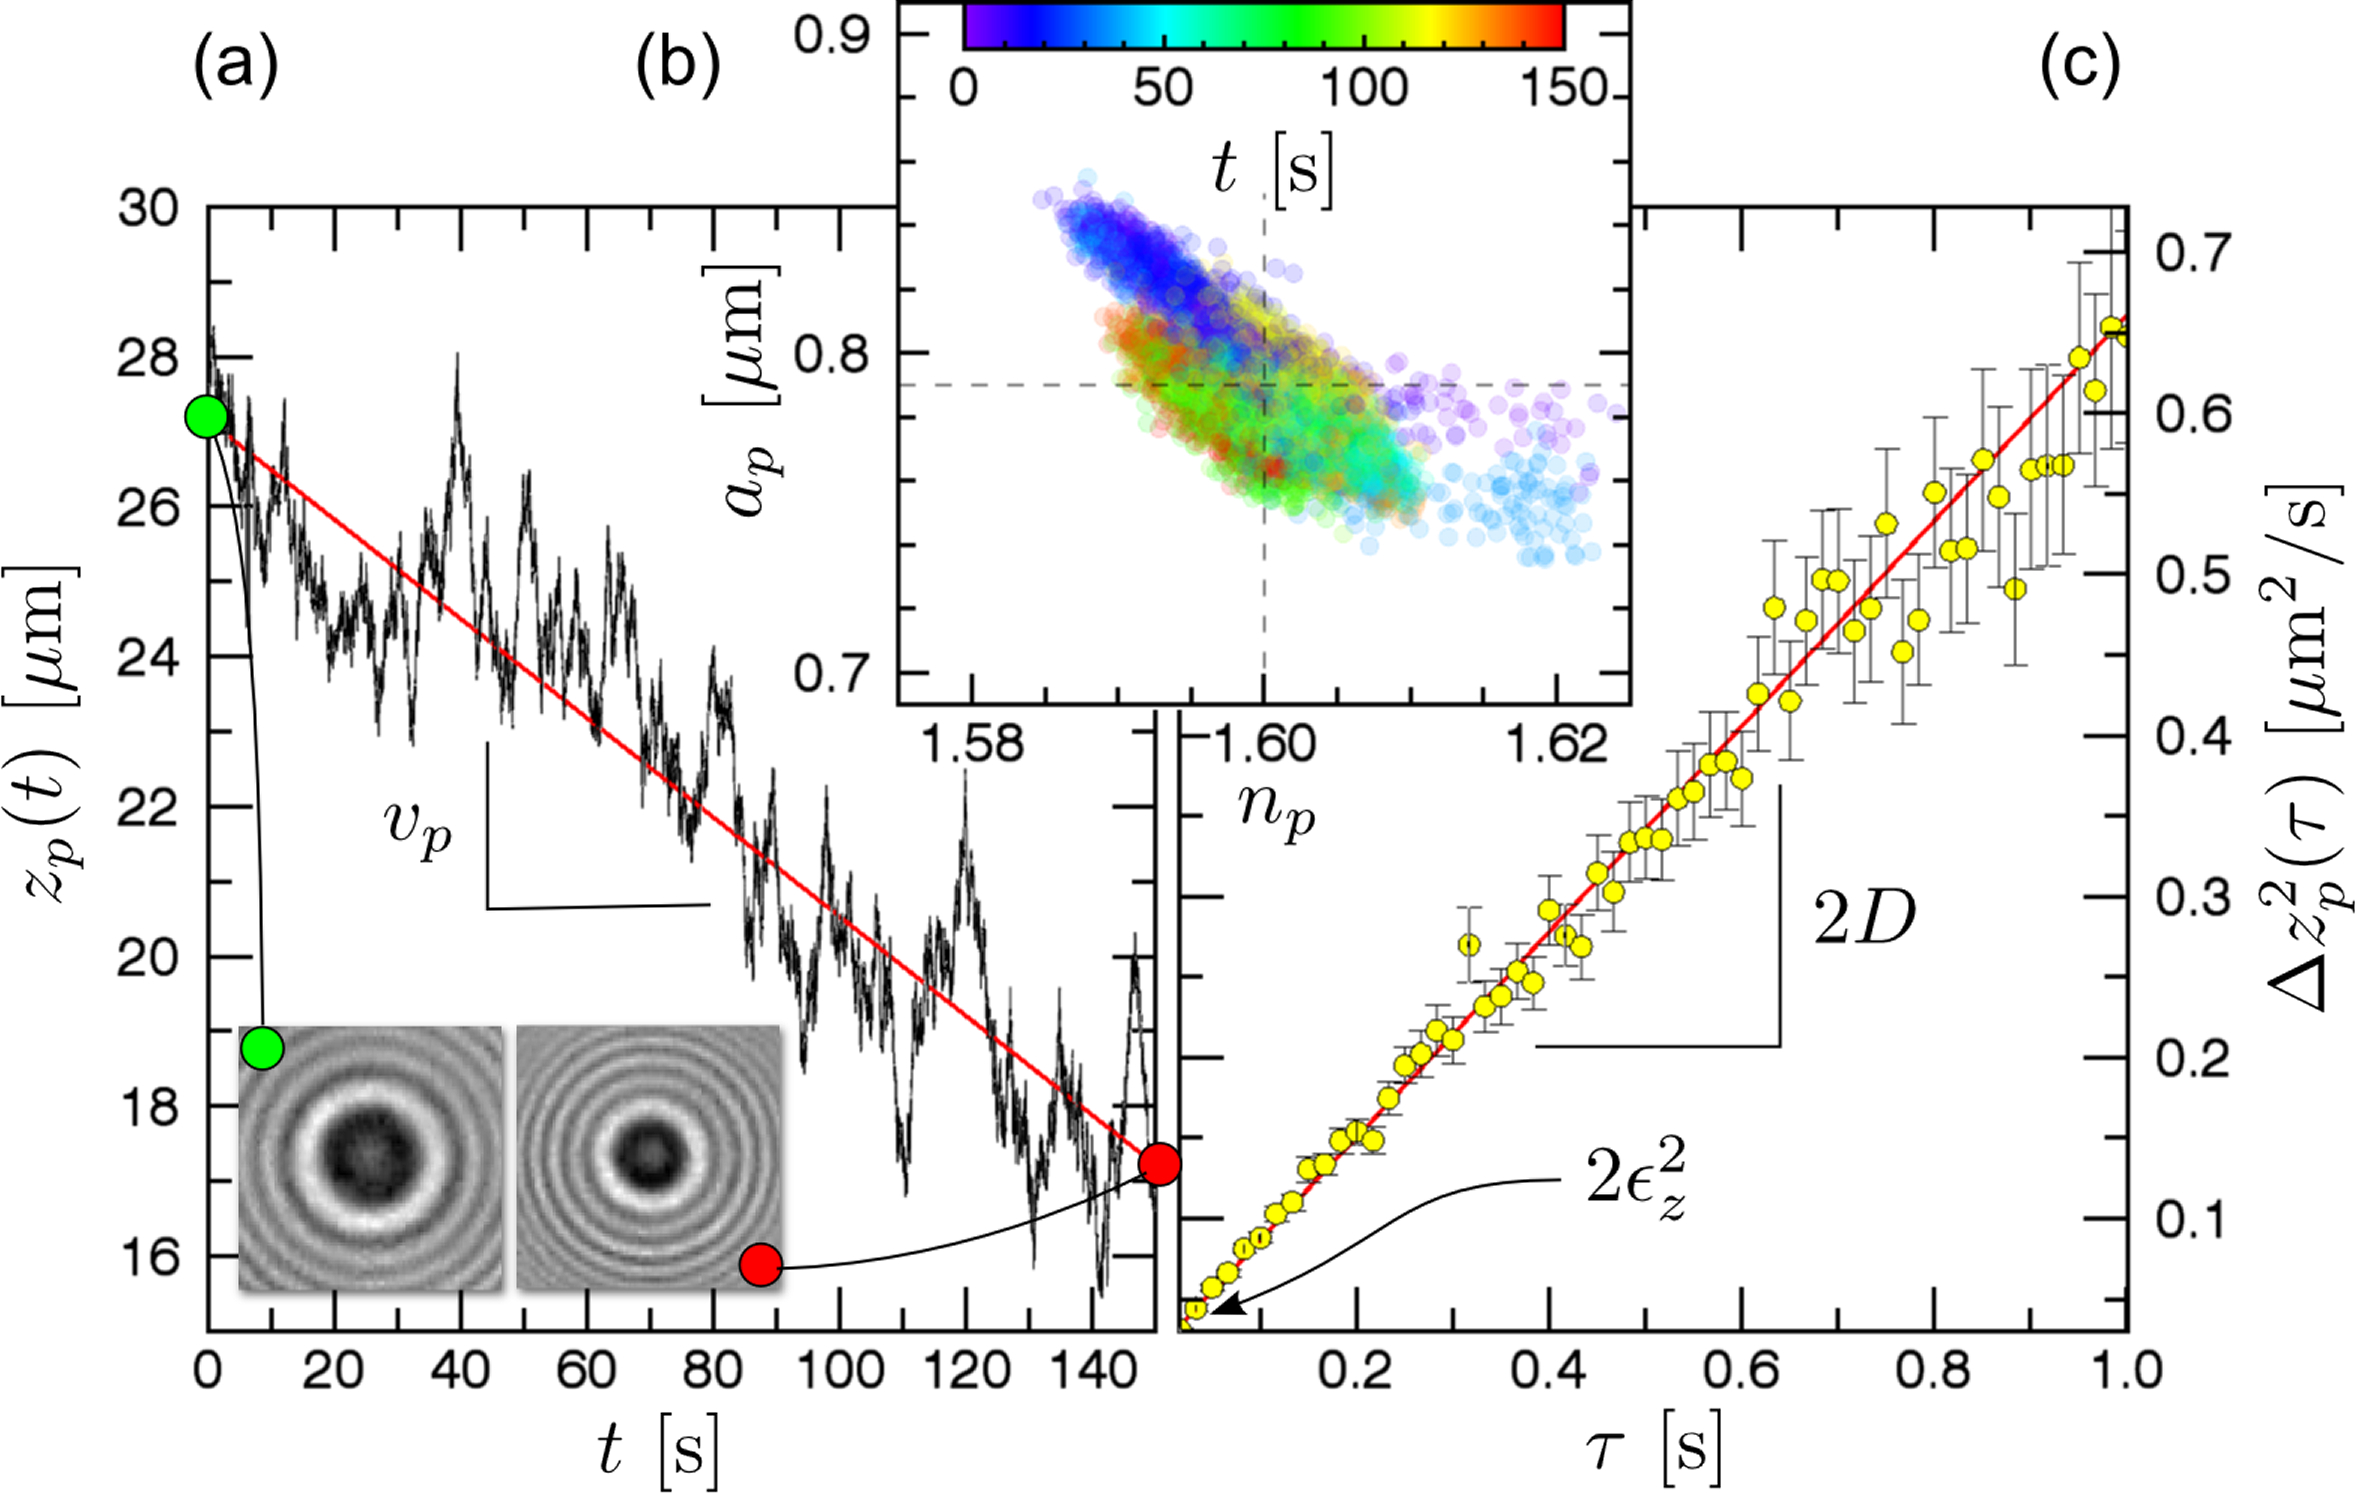
\includegraphics[width=\textwidth]{svr_figure2}
  \caption{Tracking and characterizing a single colloidal sphere.
    (a) The estimated axial position, $z_p(t)$, relative to the focal plane
    of the microscope of a single polystyrene sphere sedimenting
    through water as it diffuses.  The line is a least-squares fit.
    Insets show the sphere's hologram at the beginning and end
    of the trajectory.
    (b) The radius, $a_p$, and refractive index, $n_p$,
    estimated from each hologram in the same sequence, colored
    by time.  Each dot corresponds to values obtained from a single
    hologram.
    (c) The mean-squared displacement, $\Delta z_p^2(\tau)$, as a function
    of lag time $\tau$ computed from the data in (a), including
    statistical error bars.  The superimposed line is a fit to
    Eq.~\eqref{eq:einsteinsmoluchowsky} \cite{yevick14}.}
  \label{fig:values}
\end{figure}

Tracking a single colloidal sphere as it sediments and diffuses
provides insights into
the precision and accuracy of SVM-mediated holographic characterization.
The data in Fig.~\ref{fig:values} were obtained with
a \SI{1.59}{\um}-diameter
polystyrene sphere (Duke Scientific, catalog 4016A)
diffusing as it sedimented through
deionized water near the midplane of
a \SI{120}{\um}-deep channel.
Figure~\ref{fig:values}(a) shows the time-resolved
trajectory, $z_p(t)$, obtained from a sequence of \num{4,500} video frames
recorded at \SI{29.97}{frames\per\second}.

Because polystyrene is roughly 5 percent more dense than water,
the sphere sediments
more that \SI{10}{\um} over the
course of the experiment.
The insets to Fig.~\ref{fig:values}(a) show how markedly
the hologram's appearance changes from the beginning
of the trajectory to the end.
Despite these changes, the SVMs' estimates for the
radius and refractive index plotted in Fig.~\ref{fig:values}(b)
remain clustered around the mean values,
$a_p = \SI{0.79(2)}{\um}$
and 
$n_p = \num{1.600(6)}$.

Uncertainties in estimated parameters are computed as
standard deviations of the distribution of results
plotted in Fig.~\ref{fig:values}(b).
These should be interpreted with care because errors in SVM estimates
need not be independent or normally distributed.
Data points in Fig.~\ref{fig:values}(b) cluster around
different values as the particle descends,
which suggests that different support 
vectors dominate the estimates for $a_p$ and $n_p$
when the sphere is at different axial positions.
Systematic errors in the individual parameters therefore may 
vary with changes in any of the parameters' values.
Even so, the averages of the SVM estimates
are consistent with the manufacturer's specifications,
and differ only slightly from those obtained
with a full Lorenz-Mie analysis of the same data set
\cite{krishnatreya14},
which yields $a_p = \SI{0.805(1)}{\um}$ and
$n_p = \num{1.5730(6)}$.
Nonlinear fitting offers ten times better precision and
accuracy \cite{krishnatreya14}.
SVM analysis is a thousand times faster.

The mean sedimentation speed,
$v_p = \SI{66(1)}{\nm\per\second}$,
estimated from the slope of $z_p(t)$ is somewhat smaller than the value measured with
fits to the Lorenz-Mie theory
\cite{krishnatreya14} of $\SI{75(1)}{\nm\per\second}$.
This discrepancy further suggests that the SVM estimate for a
parameter's value may depend on the value itself.
If we nevertheless assume that errors in $z_p$
are normally distributed with a root-mean-square value $\epsilon_z$,
then the diffusing particle's mean-squared
displacement should evolve over time interval $\tau$ as
\begin{equation}
  \Delta z_p^2(\tau)
  \equiv
  \avg{ \left[ z_p(t + \tau) - z_p(t) \right]^2 }_t
  =
  2 D \tau + v_p^2 \tau^2 + 2 \epsilon_z^2,
  \label{eq:einsteinsmoluchowsky}
\end{equation}
where $D = k_B T / (6 \pi \eta a_p)$ is the Stokes-Einstein
value for the particle's diffusion coefficient.
The data in Fig.~\ref{fig:values}(c) yield
$D = \SI{0.319(4)}{\um\squared\per\second}$, which
is slightly larger than the value of
\SI{0.292(4)}{\um\squared\per\second}
obtained with the full Lorenz-Mie analysis \cite{krishnatreya14}.
The best-fit tracking error,
$\epsilon_z = \SI{107(2)}{\nm}$, exceeds the Lorenz-Mie
bound by an order of magnitude \cite{krishnatreya14}.

\section{Discussion}

The results presented here are typical of the performance of SVMs
for characterizing and tracking colloidal spheres with a wide
variety of compositions and sizes moving over a large axial range.
The speed and precision of SVM characterization
is ideal for monitoring, feedback control and quality assurance
in any industrial process involving colloidal spheres.
In applications where the greatest precision is required, parameters
estimated with SVMs can be used to initialize nonlinear least-squares
fits.
Starting from such reasonable estimates speeds convergence and
reduces the likelihood of failed fits.
Being able to resolve multimodal distributions
by quickly amassing single-particle measurements
avoids ambiguities inherent in population-averaging
methods such as dynamic light scattering.
Extracting the refractive index as well as the size offers
insights into sample composition that otherwise would
not be available.
SVM-accelerated tracking can be used for real-time
three-dimensional particle-tracking velocimetry \cite{cheong09}.
For applications such as microrefractometry \cite{shpaisman12},
the medium's refractive index, $n_m$, can 
be estimated instead of the particle's.

This combination of capabilities enables new applications.
For example, the distribution of properties in colloidal mixtures
could serve as fingerprints for complex fluid systems, with the
sizes, refractive indexes and relative abundances encoding information
that can be accessed with SVM-mediated holographic
characterization.

Such applications can be realized with comparatively
simple instruments \cite{krishnatreya14} conveying image data
to low-power computers.
Although training SVMs can be computationally intensive,
the data comprising a set of trained SVMs occupies less
than \SI{100}{\mega byte}.
Pre-computed SVMs therefore can be archived and rapidly
retrieved when needed.
This approach lends itself to
implementation on embedded computers for integration into
low-cost analytical instruments.

Other machine-learning techniques also might be effective
for analyzing holograms of colloidal particles.  Artificial
neural networks, for instance, can be trained in the same
manner as the present SVM implementation to interpret
radial profiles of experimental holograms.  SVMs have the advantage
that their training process proceeds deterministically, and therefore
tends to be faster.  Once successfully trained, however, artificial
neural networks are generally more computationally efficient.
Regardless of implementation, the present results demonstrate
that machine-learning methods facilitate
fast and precise measurements of colloidal properties.

This work was supported by a research grant from Procter \& Gamble.

    \newpage
    
    \chapter{Optimizing the synthesis of monodisperse colloidal spheres}
\label{ch:synthesis}

\section{Introduction}

The earliest reference to synthetic emulsion polymerization dates back to
1909 \cite{bayer1909,finch03} to a patent awarded to Felix Hoffmann and
co-workers at Farbenfabriken Bayer for their pioneering work in producing
synthetic latex.
Techniques for polymerizing emulsions have progressed through
intuitive leaps guided by fundamental principles of chemistry
and physics.  Quite often, the importance of particular chemical
or physical conditions to the outcome are gauged once
synthesis is complete, and requires multiple orthogonal measurement
techniques. Examples include measurements of the particles' size distribution,
their surface texture, and their porosity.

Holographic particle
characterization can streamline this analysis by providing particle-resolved assays
of samples' size distributions and composition rapidly and with
minimal sample preparation.

Holographic assays provide information that is useful for designing synthetic
pathways and can help to detect and diagnose deficiencies. These measurements
can proceed rapidly enough, moreover, to provide real-time feedback during
synthesis. We illustrate these capacities by analyzing the synthesis of a
particularly interest colloidal suspension.

In this chapter we use holographic particle characterization
to explore the role of stoichiometry, initiator choice, and
agitation conditions on the synthesis of monodisperse spheres of
\num{3}-methacryloxypropyltrimethoxysilane (TPM) \cite{vanderwel17},
a model system with increasingly widespread applications
in soft-matter research \cite{sacanna11,liu16,vanderwel18}.
We employ holographic particle characterization
in tandem with conventional particle characterization
techniques to identify factors that 
influence size selection, polydispersity, and surface texture.
Complementary analysis serves to validate results obtained by
HPC.

\section{Synthesizing TPM spheres}
% FIXME: Possibly meld the previous paragraph and the next.%

TPM spheres are a particularly useful model system for colloidal studies.
A comparatively straightforward synthesis readily produces monodisperse spheres
with selective sizing between from a few hundred nanometers to a few micrometers
\cite{liu16}.
Unlike the better-known syntheses polystyrene \cite{goodwin1974} and silica \cite{stober68},
TPM particles require no specialized equipment or inert environment necessary.
However, there are many parameters in the synthesis that can affect the average size and refractive
index for a synthesized population. This chapter describes how holographic particle
characterization can guide the synthesis of TPM spheres by elucidating how
synthesis conditions affect the properties of synthesized particles.
Our work builds on the work of van der Wel \emph{et. al} \cite{vanderwel17} that
uses conventional characterization techniques to systematically
characterize the emulsion polymerization protocol for TPM spheres.

Our procedure for synthesizing TPM spheres is described in section
\ref{ssec:synthesizing_tpm} with the
exception of initiator choice. We reiterate the synthesis protocol
here to underscore the conditions we varied and to enumerate the
\num{32} samples of droplets and polymerized spheres we analyzed.
A detailed account of the polymer chemistry underlying this
protocol is provided in Ref.~\cite{vanderwel17}.

\subsection{Emulsion polymerization}
\label{ssec:polymerization}
Controlling the size, monodispersity, and composition of colloidal spheres is crucial
for many applications including colloidal crystallization \cite{pusey87} and micrometer scale
self-assembly \cite{sacanna11}. In this study 
we investigate the influence of stir rate, concentration of ammonium chloride,
concentration of TPM oil, and radical initiator choice on the size and refractive index
of the manufactured particles. To do so, we prepared numerous batches of TPM particles
with independent deviations from the above synthesis protocol and
characterized the resulting particles with holographic particle characterization.

The synthesis begins with the formation of an emulsion of monodisperse TPM droplets.
Monomeric TPM, ((3-(Trimethoxysilyl)propyl methacrylate, \SI{98}{\percent}, Sigma Aldrich)
which is insoluble in water, is added to a basic environment
(pH $>$ \num{9}) of ammonium chloride (\SI{29}{\percent}) in water.
The monomers undergo hydrolysis in water and become water soluble. 
In a basic environment, these hydrolyzed monomers form insoluble 
oligomers. As the suspension is stirred, the oligomers condense 
homogeneously into monodisperse droplets that continue to grow as more oligomers form.
After \num{2} hours, the abundance of free hydrolyzed monomer is depleted
causing oligomerization to halt and therefore droplet growth to cease.
The emulsion is then heated to \SI{80}{\degreeCelsius} and a free radical 
initiator is introduced to polymerize the droplets and form solid spheres.

The dissociation of ammonium chloride in water leads to the production of ammonia
gas,which escapes the solution lessening its pH.
To mitigate this effect, emulsion formation is completed in a closed vial.
Additionally we use identical \SI{12}{\milli\liter} vials to produce \SI{5}{\milli\liter}
of colloidal suspension in each synthesis so that the amount of enclosed air, and therefore
loss in pH, is consistent across samples. Identical stir bars are used for all syntheses
to ensure consistent flow properties.

\subsection{Holographic particle characterization}

We perform holographic characterization measurements with a Spheryx xSight,
a commercial holographic particle characterization system
that automates the methods described in the previous chapters.
The xSight flows a colloidal suspension through the observation volume of a conventional microscope
and illuminates the suspension with a laser operating at a vacuum wavelength of \SI{532}{\nm}.
The proprietary software and hardware implemented in
the instrument yield the size and refractive index for each observed colloidal spheres and
does so in a fraction of the time we typically spend analyzing an experimental video.
Because we are only interested in collecting population statistics for the size and refractive
index of our colloidal systems, we utilize the xSight rather than our custom-built microscope.

The xSight analyzes colloidal dispersions with particle number densities below 
\SI{E6}{\milli\liter^{-1}} to reduce the occurrence of overlapping holograms.
This is consistent with our discussion in section \ref{ssec:sample_prep}.
The emulsification polymerization process described in section \ref{ssec:polymerization}
produces a sample with a number density of \SI{E10}{\milli\liter^{-1}}.
We therefore dilute each of our samples by a factor of \SI{E4}{} with
deionized water.
%We utilized xCells, the flows cells designed for the xSight, with each flow
%analyzing \SI{3}{\micro\liter} of sample passing through a \SI{50}{\um} deep observation volume;
%this provides us with scattering information of a few thousand colloidal spheres per sample.

We analyze \SI{3}{\micro\liter} of each sample by pipetting the diluted dispersion into an
xCell sample cell and loading the xCell into the xSight. The xSight draws the fluid through
the xCell's \SI{50}{\um} deep observation volume. A ten-minute measurement provides us with
characterization data for a few thousand colloidal spheres per sample.

\begin{figure}
    \centering
    \includegraphics[width=\columnwidth]{example_poiseuille_fit}
    \caption{The measured flow profile of particles streaming through the xCell.
      (a)  A diagram of the observed Poiseuille flow.\protect\footnotemark 
      (b) Scatter plot of average particle height and average velocities; each
      dot represents a single micrometer scatterer. Color denotes the density of
      observations. The fit to a parabolic flow profile is illustrated with a dashed
      blue line. (c) Scatter plot of data after filtering observations deviating
      from the parabolic profile.}
    \label{fig:flow_prof}
\end{figure}

\footnotetext{The focal plane is only \SI{90}{\um} below the lower sample-xCell interface:
  a to-scale diagram would depict the focal plane inside the lower xCell wall.}
The dilute suspension is pumped between the stationary walls of the xCell.
The resulting fluid flow takes on a parabolic profile known as a Poiseuille flow.
As the system is in a low-Reynolds number flow, every colloidal sphere traces
the flow of the fluid.
As illustrated in Fig.~\ref{fig:flow_prof}(a), the xCell's walls are located
at \SI{90}{\um} and \SI{150}{\um} relative to the xSight's focal plane.
Because the xSight records the mean $z$-position and mean 
velocity of all multiply-imaged scatterers, we are able to fit the flow
profile to a Poiseuille flow as depicted in Fig.~\ref{fig:flow_prof}(b).
The majority of observations fall neatly onto the parabolic profile. 
Some fits however deviate markedly. Presumably these data result from fitting
false positive detections of overlapping holograms.
We suppress these erroneous features by filtering data that deviate from
the parabolic profile by more than one median absolute deviation
as depicted in Fig.~\ref{fig:flow_prof}(c).

\subsection{Orthogonal validation methods}


We used scanning electron microscopy to provide baseline estimates of the
particles against which to compare holographic characterization measurements.
Each sample of polymerized spheres were imaged with a MERLIN (Carl Zeiss) field
emission scanning electron microscope (SEM).
Typical images are provided in Fig.~\ref{fig:synthesis_stir_rate}(a).
SEM images provide a visual check on the sample's uniformity
and can be used to estimate the colloidal spheres' diameter. While a well calibrated scanning
electron microscope provides \num{1} to \SI{10}{\nm} resolution of features, sample
preparation, particularly vacuum decompression and sputter coating, can shrink or
even swell the sample \cite{yamada85,jung02}. The liquid TPM droplets
are not amendable to SEM analysis.

\section{Results}
\subsection{Effect of stir rate}

Stirring the sample while the oligomers condense into droplets suppresses coalescence and
promotes homogeneous nucleation by uniformly dispersing the hydrolyzed monomer and droplet
nuclei. %%FIXME CHECK THIS STATEMENT.
The effect of stir rate on the resulting particle size is, however, less clear;
we investigated the influence of stir rate by producing \num{4} sets of TPM emulsions.
In four identical vials with identical stir bars, we placed \SI{15}{\milli\liter} of 
\SI{29}{\percent} ammonia followed by \SI{200}{\micro\liter} of TPM 
monomer to \SI{5}{\milli\liter} of DI water. The four samples were then stirred 
using magnetic stir plates set at \num{500}, \num{700}, \num{900}, and
\SI{1100}{\minute^{-1}} for \SI{2}{\hour}. % XXX Use rpm instead of min^{-1}?
The droplets were then polymerized by adding
\num{2},\num{2}'-azobis(\num{2}-methylpropionitrile, Sigma Aldrich) (AIBN) as a radical initiator and %FIXME: Lot number of AIBN?
heating the sample to \SI{80}{\celsius} for \SI{2}{\hour}.
We prepared a sample of the unpolymerized droplets and a sample of polymerized TPM spheres
at each of the four spin rates, for a total of eight samples.

The result of holographic particle characterization for the \num{4} polymerized samples
and the \num{4} unpolymerized samples are summarized in Fig.~\ref{fig:synthesis_stir_rate}(b).
Each dot represents the average size and refractive index for the associated sample. Error
bars represent the single median absolute deviation of the associated property.
The unpolymerized droplets, represented with dashed error, bars have a systematically
lower refractive index than the polymerized droplets, represented with solid error bars.
Polymerization changes the chemical makeup of the droplet and generally increases the
density; both processes might reasonably account for the observed increase.
Both values greatly exceed the refractive index of bulk TPM oil, which is indicated by
a dashed line in Fig.~\ref{fig:synthesis_stir_rate}(b).
Hydrolysis and oligomerization of TPM oil account for three quarters of
the total change 

Digital SEM images were analyzed with ImageJ to estimate the diameters of \num{10}
spheres from each sample.
The average particle diameters were \SI{1.48}{\um}, \SI{1.63}{\um},
\SI{2.03}{\um}, and \SI{1.82}{\um} for stirring rates \num{500}, \num{700}, \num{900}, and
\SI{1100}{\minute^{-1}} respectively. We note that the SEM images for the emulsion
stirred at \SI{1100}{\minute^{-1}} reveal a small population of \SI{100}{\nm}.

\begin{figure}
    \centering
    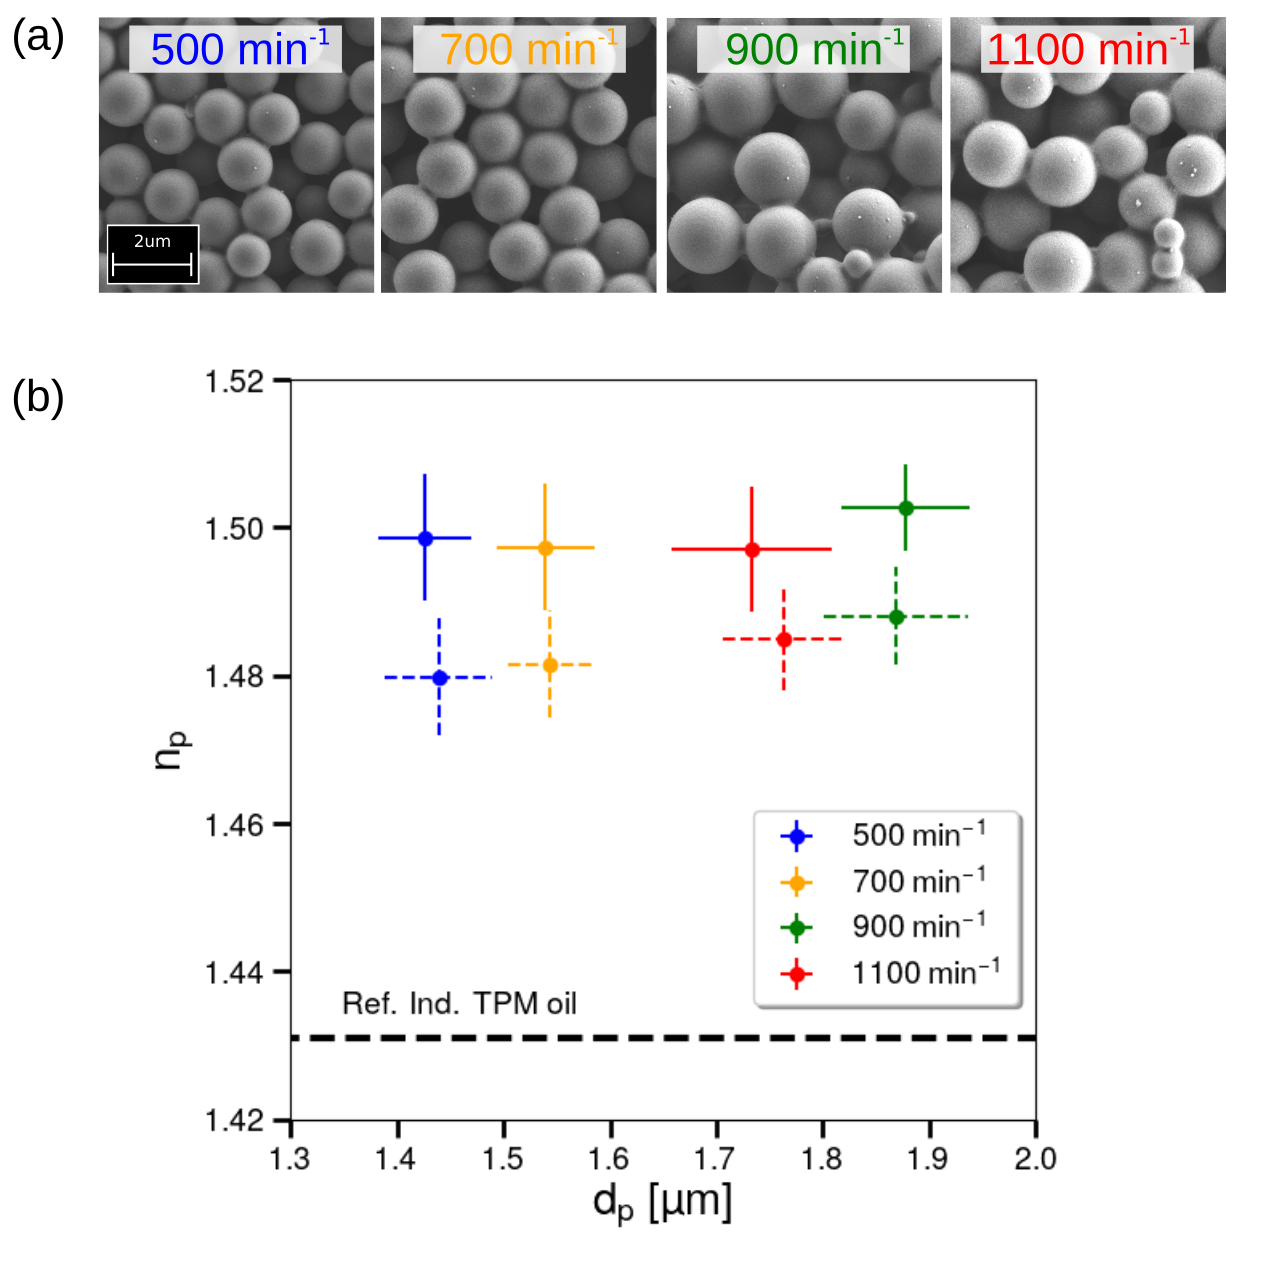
\includegraphics[width=\columnwidth]{synthesis_stir_fig}
    \caption{(a) Cropped and scaled SEM images of the polymerized TPM spheres whose
      samples were stirred at \num{500}, \num{700}, \num{900}, and \SI{1100}{\minute^{-1}}.
      (b)  The result of HPC analysis for the unpolymerized and polymerized
      emulsions stirred at \num{4} different rates. Solid-lines represent the polymerized
      spheres; dashed-lines represent the unpolymerized droplets; color differentiates the sample by
      spin rate. Each dot represents the
      average diameter and refractive index for a sample. Error bars are set by a single
      median absolute deviation of the measured property for a given sample. The dashed
      black line provides reference to the refractive index of monomeric TPM oil.}
    \label{fig:synthesis_stir_rate}
\end{figure}


\subsection{Effect of heat bath exposure time}

This synthesis of TPM employs heat-activated free-radical initiators to polymerize TPM droplets:
time spent thermally coupled to a heat bath greatly accelerates polymerization.
As observed in Fig.~\ref{fig:synthesis_stir_rate}, the polymerization of
liquid TPM droplets can induce a shift of approximately \SI{0.02}{} in refractive index
which is well within the precision of the xSight.  Because the refractive index
of a material is a function of its composition \cite{wang15},
refractive index serves as a proxy for the degree of
polymerization of a sample.  Holographic particle
characterization is uniquely poised to probe the time dependent polymerization of TPM as
it can monitor the refractive index of individual spheres \emph{in situ}.

We investigate the polymerization rate of TPM droplets by regularly sampling a
suspension undergoing polymerization and characterizing each drawn sample with HPC.
Specifically, the suspension consists of an emulsion of TPM droplets
and the initiator AIBN. The suspension is continuously stirred at \SI{1100}{\min^{-1}}
and is thermally coupled to a heat bath set at \SI{80}{\degreeCelsius}.
We drew \SI{1}{\ul} of the suspennumon after \num{0}, \num{5}, \num{10}, \num{15},
\num{20}, \num{40}, and \SI{60}{\min}. Each sample is added to \SI{1}{\ml} of
room temperature DI water, which effectively arrests any continued polymerization.
Each sample is then immediately characterized by the xSight. Figure ~\ref{fig:heat_size_time}
depicts the result of this chacterization.
%XXX (Add conclusions about polymerization time- only takes maybe 15 min?)


\begin{figure}
    \centering
    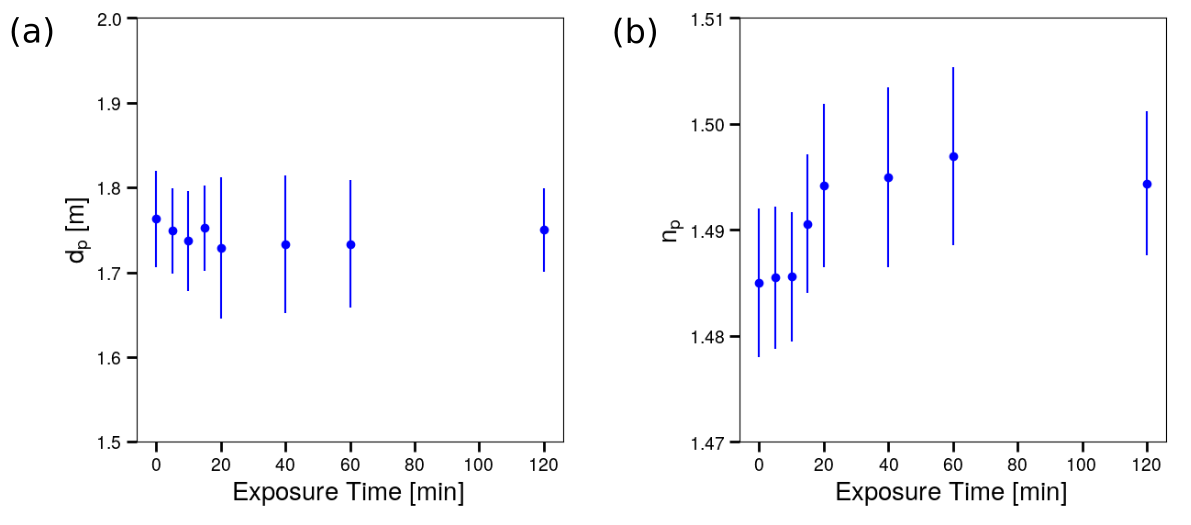
\includegraphics[width=\columnwidth]{synthesis_heat_bath}
    \caption{Particle properties after heat bath exposure times of \num{0}, \num{5},
      \num{10}, \num{15}, \num{20}, \num{40}, and \SI{60}{\min}.
      (a) The average size and (b) refractive index of particles as a function
      of heat bath exposure time. Error bars indicate a single median absolute deviation
      of the associated property.}
    \label{fig:heat_size_time}
\end{figure}

Fig.~\ref{fig:heat_size_time}(a) demonstrates that any changes in size are below
the polydispersity in size. Fig.~\ref{fig:heat_size_time}(b), however, demonstrates
a large shift in refractive index. The first ten minutes are nearly identical;
presumably this is while the suspension is equilibrating with the heat bath.
At \num{15} and \SI{20}{\min} the refractive index significantly increases.
van der Wel \emph{et. al} \cite{vanderwel17} suggest heating the suspension
for \SI{2}{\hour} to ensure the sample has sufficiently polymerized and is
stable. Our analysis suggests that a much shorter time may suffice although
we have not confirmed the resulting stability of the polymerized sample.



\subsection{Effect of stoichiometry and choice of free-radical initiator}

To probe the variables of droplet formation, we make four batches of droplets.
In each case we hold the volume of water, \SI{5}{\milli \liter} constant 
and vary the amounts of TPM and ammonia. Batches A and B each had 
\SI{100}{\micro\liter} of TPM with \si{10} and \SI{20}{\micro\liter} of 
ammonia added, respectively. Batches C and D had \SI{150}{\micro\liter}, 
again with \si{10} and \SI{20}{\micro\liter} of ammonia, respectively. 
\SI{0.1}{\percent} sodium docecyl sulfate (SDS) was introduced to
each sample to suppress aggregation. Through this, we can observe the effects of
varying the amount of TPM and the pH on the size of the resulting droplets.
This gives 
% XXX (Add conclusions about initiator- does not seem to matter)

Next, we observe the effect of using different free radical initiators 
to polymerize the particles. Two water-insoluble initiators, AIBN and
\num{1},\num{1}'-azobis(cyclohexanecarbonitrile) (ACHN), and two water-soluble 
initiators, potassium persulfate (KPS) and ammonium persulfate APS), were 
used.

To compare initiators, one \SI{5}{\milli \liter} suspension of emulsion droplets is
made in a \SI{12}{\milli \liter} vial and then equally divided into five
\SI{1.5}{\milli \liter} microcentrifuge tubes. One tube was left unpolymerized. The
other four tubes were then polymerized at \SI{80}{\celsius} 
for \SI{12}{\hour} on a shaker at \SI{750}{\minute^{-1}} % XXX Again, rpm vs mins^{-1}
to prevent sedimentation.
We added a different free radical initiator to each tube and repeated the process with four
different emulsions for a total of 
\num{16} measurements to ensure that any observations were the result of the 
initiator used and not of the particular protocol used to make the emulsion.


% Van Der Wel et. al suggest that the density increases by 1.07 during polymerization.
% IF the mass stays the same, this corresponds to a 2% decrease in radius.
% For a 1.5 um diameter TPM sphere, a 2% decrease reduces the size to 1.46 um.
% That would be visible in our 

\begin{figure}
    \centering
    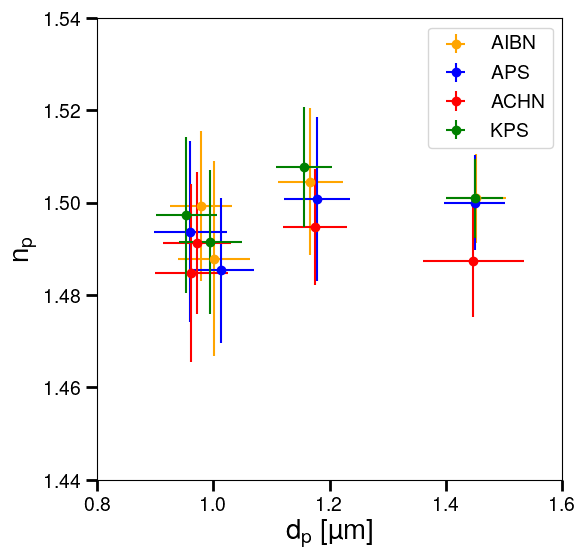
\includegraphics[width=0.75\columnwidth]{may_data_summary.png}
    \caption{The refractive index and diameter of 16 samples of 
    polymerized TPM.}
    \label{fig:initiator_data}
\end{figure}

In making the \si{16} sets of particles to look at the effect of initiator on 
the particles, we can also make observations about the effects of varying 
the amount of TPM and the pH on the size of the resulting droplets. To hold 
the pH constant, we can compare sample A to C and sample B to D. This gives 
the fairly intuitive result that increasing the amount of TPM increases the 
size of the final droplet. Holding the amount of TPM constant and varying 
the pH, which means comparing A to B and C to D, shows that increasing the 
pH of the environment during droplet formation decreases the size of the 
final droplet. This is less intuitive but perhaps not surprising, as the pH 
affects the rate at which oligomers form and therefore the rate of droplet 
formation. This leads to more nucleation sites and therefore smaller droplets 
for the same volume of material. 

Comparing batches A to C, each with \SI{100}{\micro \liter} of TPM monomer, and B to D with
\SI{150}{\micro \liter}, gives the somewhat intuitive result that increasing the amount of TPM
monomer increases the size of the final droplet. On the other hand, comparing A to B with
\SI{10}{\micro \liter} ammonia and C to D with \SI{15}{\micro \liter} ammonia shows that
increasing the pH of the environment during droplet formation decreases the size of the 
final droplet. This is less intuitive but perhaps not surprising, as the pH 
affects the rate at which oligomers form and, therefore, the rate of droplet 
formation. Increasing the pH results in more nucleation sites and therefore smaller droplets 
for the same volume of material. 

Under certain conditions, TPM droplets are known to form dimpled spheres when polymerized with
the water-soluble initiators APS and KPS due to the ejection of low molecular weight oligomers
(citation- I forget which of Stefano's papers?). Therefore, one might think that TPM spheres
polymerized with these initiators would be made of on average higher molecular weight oligomers
and have a higher refractive index than pa. However, under the conditions observed here where no
dimple was formed, there was no observable difference in particle size or refractive index between
the initiators used.

\section{Discussion}

\section{Acknowledgment}

This work was supported primarily by the MRSEC program of
the National Science Foundation through Award Number DMR-1420073.
Additional support was provided by the SBIR program of the
National Science Foundation through Award Number IPP-1519057.
The FESEM was purchased with financial support from the MRI program
of the National Science Foundation under Award DMR-0923251.

\% FIXME David please check the acknowledgment

    \newpage
    
    \chapter{Conclusions}
\label{ch:conclusion}



This thesis validates, extends, and employs holographic
particle characterization, a relatively new technique
for extracting the position, size, and composition
of micometer-scale scatterers \emph{in situ}. This
thesis advances the technique by providing a
firm foundation for the scalar-wave approximation
in image formation and introduces the effective
sphere model which expands its domain of applicability.
In addition we implement machine learning algorithms for
detecting, localizing, and characterizing holograms; these
advances greatly reduce the computation time and enable of
the real-time analysis of dense, heterogeneous samples.
We then use the technique to investigate the role of
environment conditions and chemical choices in
a specific emulsion polymerization process.

In \autoref{ch:debye} we justified the use of the scalar theory
approximation is outlined in \autoref{ch:hvm}.
Where possible, we accounted for the vectorial nature
of light propagation including reflection, refraction,
angular demagnification, and polarization rotation
through the elements of the optical train. By fitting synthetic holograms
based on a vector-based theory to a scalar theory,
our simulations determined that for scatterers between \SI{0.5}{\um}
and \SI{10}{\um} with refractive index between \SI{1.4}{} and \SI{1.7}{},
the scalar theory is provides the same prediction as a vector-based theory,
albeit with far less computational overhead. 

Fitting holographic features to the Lorenz-Mie theory
assumes a homogeneous spherical scatterer and yet colloidal particles
come in many shapes such as aggregates, clusters and rods. In \autoref{ch:dimpled}
we presented a series of experimental and simulated results that demonstrate
that the Lorenz-Mie theory provides a first-order approximation for light scattering
off of aspherical particles. For micrometer sized particles with small deviations
from a spherical geometry, fitting to the Lorenz-Mie theory measures
an effective size and refractive index.

In \autoref{ch:cascade} we considered the first step in analyzing recorded
images: detecting and localizing holographic features. We trained two machine
learning algorithms, a cascade classifier and a convolutional neural network (CNN),
to accomplish these tasks. We compared these two techniques against previously
employed heuristics for precision, recall, and speed. Our tests demonstrate that
the CNN and cascade respectively boast speeds-ups of \num{10} and \num{100} times
faster processing than our heuristics. The CNN can robustly detect and accurately
localize highly overlapping, high-contrast features with exceedingly few false positives.
The Haar-based cascade classifier provides single-pixel rather than
sub-pixel precision yet its speed and modest computational requirements provide
real-time localization and detection abilities. We demonstrated that the cascade
classifiers can operate as a high-speed targeting system for a holographic
optical trapping system where single-pixel precision suffices to capture
rapidly diffusing targets.

\autoref{ch:svr}

\autoref{ch:synthesis}


    \newpage

    %%%%% Appendices start %%%%%%%%%%%%%%%%
    %% Comment out the following line if your thesis has no appendix
    % \appendix
    
    %If you have only one appendix copy this line out
    %% \phantomsection
    %% \addcontentsline{toc}{chapter}{Appendices}
    
    % 
    % If you have multiple appendices, they shouldn't individually appear
    % in the table of contents, but rather be listed in the List of
    % appendices. To do this, put the following code(defined in
    % definitions.tex) at the front of each appendix file(Tip from Jan Smrek):
    %
    % %\SkipTocEntry\chapter{Appendix Title} 
    % %\label{app:appendixtitle}
    % %\appcaption{\thechapter \space Appendix Title}
    %
    %
\subsubsection{Digitizing Images}
\label{ch:hvm:sec:hvm:ssec:digitalrec:sssec:digitizing}

Modern digital cameras employ an array of photon detectors to measure the
average intensity over the sensor surface. Each photon detector, referred to as a pixel,
utilizes the photoelectric effect to convert photons into excited electrons.
The excited electrons at each pixel are counted, sometimes to single precision, and
then digitized into $8$-, $12$-, or even $16$-bit integers. Because the number of
excited electrons is proportional to the number of photons, and the the number of
photons is in turn proportional to the intensity of the of the image at the
sensor surface, the array of electron counts serves as a proxy for the intensity
of the image.

With millions of pixels and the capacity to count tens of thousands of electrons at each pixel,
digital cameras are an engineering marvel. For our purposes, we will review a few of the physical
details of a single pixel to explain important imaging effects such as dark counts, saturation,
and the digitization procedure.

Pixels are designed to accurately count the number of electrons that are
excited by incident photons within a given exposure period. A number of physical constraints
limit the accuracy of each pixels.

During an exposure period, $N_p$ photons of a particular wavelength arrive at a pixel
surface. Some fraction of the incident photons are converted to excited electrons
with a wavelength dependent probability known as the quantum efficiency. To be properly
counted, these excited electrons must survive until the counting procedure has
accounted for their presence. To this end, each pixel is doped to increase the lifetime
of excited electrons. In addition, the excited electrons must remain in the bulk so that
they are not grounded; for this purpose, a biased field is applied. % FIXME: What about mirror charges?

During the exposure period, a number of electrons can be thermally excited (as opposed to
photonically excited) and will be included in the count. These erroneously
counted electrons are referred to as a dark count. Measuring the average dark count of a
camera is as easy as recording the average image while an opaque object is blocking the
camera's sensor. Note that the dark count will increase with the length of the exposure
period.

% The number of electrons that can be negative.. scientific cameras have a non-zero
% floor to maintain gaussian-errors.
% Saturation occurs because the relation number of excited electrons per
% number of incident photons becomes non-linear. The largest number of reported
% electrons is the highest level

% A number of approximations come to mind with the LM theory.
% Approximation of radial component
% Approximation of functional form (Hankel function)
% Approximation of polarization



\subsection{Digital Recording}
\label{ch:hvm:sec:hvm:ssec:digitalrec}

% What are digital images. How are digital images recorded?
% Why are you telling them such things?
% How is it that digital images do not record intensity?

Images in science are ubiquitous; by sampling the intensity over an exposure
period, a single image encodes a bevy of spatial information that is ripe
for qualitative and quantitative analysis. Historically, researchers would
extract this information by hand. Jean-Perrin used a projector, pen and a paper to originally
measure the diffusion of a polymer bead. Crystallographers such as %FIXME: Add reference.
traced photographs of crystalline diffraction patterns by hand. Presently researchers utilize
digital cameras to record and digitize images as arrays of values. 

We utilize a digital camera to record holograms. To fit our experimental holograms to
theory and to simulate our digital recordings it is necessary to have a basic
understanding digital images. In this section we will 


    \begin{appendices}      
      \SkipTocEntry\chapter{Imaging with a Digital Camera} 
\label{app:digital_imaging}
\appcaption{Appendix A}

With millions of pixels and the capacity to count tens of thousands of electrons
at each pixel, digital cameras are an engineering marvel. 
A basic understanding of how digital images are recorded will elucidate
our method of image normalization and validate our model for generating synthetic
hologram images. In this appendix, we will briefly review the physical
details of a single pixel to explain important imaging effects such as
dark counts, saturation, and the digitization procedure. For a more detailed account,
consult reference \cite{nakamura2017}.

\section{Overview of digital imaging}

Digital cameras use an array of photon detectors to measure the
average intensity over the sensor's surface. Each photon detector, referred to as a pixel,
employs the photoelectric effect to convert the visible photons striking its surface into
excited electrons. The array of pixels is exposed to incoming light for a limited
exposure period, during which excited electrons accumulate at each pixel.
The excited electrons are counted, sometimes to single precision,
and digitized into $8$-, $12$-, or even $16$-bit integers. As the number of
excited electrons is proportional to the number of photons, and the the number of
photons is in turn proportional to the intensity of the image at the
sensor surface, the array of electron counts serves as a proxy for
the intensity of the image.

During an exposure period, a number of electrons can be thermally excited and
will be included in the count. These erroneously counted electrons are referred to
as the dark count. The average dark count for a specific exposure period can be measured
by blocking the camera's sensor with an opaque object and averaging the
recorded images. The resulting averaged array is called a bias frame. Note that the dark count will increase with
longer exposure times. For an exposure period of less than \SI{10}{\us}, the dark
count of our camera is less than \SI{0.5}{\percent} the average intensity 


Each pixel is designed and calibrated to closely approximate a linear relationship
between the number of photons incident on the pixel and the recorded number of
electrons excited.
This linear relationship fails, however, above a certain level of accumulated electrons
$N_{\text{max}}$.
For this reason, the registered number of electrons is limited to a maximum value; a
pixel recording this maximum response is called a saturated pixel and is reporting
a lower bound for the intensity rather than an interval of intensities.
Unbiased measurements of intensity requires that no one pixel be saturated.
For ideal holographic imaging, the illumination should therefore be set such that the brightest pixel is below its saturation level.

%During an exposure period, $N_p$ photons of a particular wavelength arrive at a pixel
%surface. Some fraction of the incident photons are converted to excited electrons
%with a wavelength dependent probability known as the quantum efficiency. To be properly
%counted, these excited electrons must survive until the counting procedure has
%accounted for their presence. To this end, each pixel is doped to increase the lifetime
%of excited electrons. In addition, the excited electrons must remain in the bulk so that
%they are not grounded; for this purpose, a biased field is applied.

% The number of electrons that can be negative.. scientific cameras have a non-zero
% floor to maintain gaussian-errors.
% Saturation occurs because the relation number of excited electrons per
% number of incident photons becomes non-linear. The largest number of reported
% electrons is the highest level

% A number of approximations come to mind with the LM theory.
% Approximation of radial component
% Approximation of functional form (Hankel function)
% Approximation of polarization

% What are digital images. How are digital images recorded?
% Why are you telling them such things?
% How is it that digital images do not record intensity?

      \SkipTocEntry\chapter{Approximations to the Lorenz-Mie Scattered fields} 
\label{app:lorenzmie_approx}
\appcaption{Appendix B}

The Lorenz-Mie theory underlies several techniques over including static light scattering
\cite{zimm48}, imaging through interstellar grains \cite{purcell1969} and sizing large
air bubbles \cite{hansen85}. In this appendix we examine the validity of
common approximations for the Lorenz-Mie scattering theory in the context of
holographic particle characterization.


\section{Validating the far-field approximation}



The light scattered by a spherical particle, $\vec{E}_s$, propagates radially and has a
non-zero, albeit decaying, radial component, $\vec{E}_s\cdot\uvec{r}$.
For many applications, the scattered wave has propagated sufficiently far that the
radial component can be safely neglected. For holographic particle characterization,
the fields may be evaluated as close as the focal plane for the scalar theory
presented in \autoref{ch:hvm} and as far as the entrance pupil for the vector-based
theory presented in \autoref{ch:debye}.
We probe the radial component's contribution to the scattered field by measuring
the its fractional contribution, $\vec{E}_s\cdot\uvec{r} \, / \abs{\vec{E}_s}$,
over a range or particle sizes and refractive indexes. The results of this analysis are
presented in Fig.~\ref{fig:radial}.



      \SkipTocEntry\chapter{Discretizing the scattered field for the Debye-Wolf integral} 
\label{app:discretize_dw}
\appcaption{Appendix C}

 \Autoref{ch:debye} presents a model for propagating the incident and
 scattered electric fields through the optical train to a digital camera.
 Eqs.~\eqref{strength_factor} through \eqref{magnification} account for the
 refraction, reflection and angular demagnification of the electric
 field strength factor up to the tube lens.
 The Debye-Wolf integral, Eq.~\eqref{eq:debye}, transforms the
 electric field strength factor at the tube lens into the electric field present in the
 imaging plane. We have implemented this transformation as a discrete Fourier
 transform as shown in Eq.~\eqref{complete_dw}. This appendix described an appropriate
 discretization of the Fourier transform such that the Debye-Wolf integral converges
 and the spacing in the image plane approximates the size of a pixel.

\section{Appropriately sampling the electric field strength factor}
  As presented in Fig.~\ref{debye_schematic}, there are three discrete grids
  necessary in 
  To ensure that
  our sampling rate will not cause aliasing, we impose the following condition on
  the sampling number $P$ (the same argument applies to the sampling number $Q$):
  \begin{eqnarray*}
    \Delta s_x &<& \frac{2 \pi}{k W_x} \hspace{.5 in} \text{Eq 142 in Ref.}\\
    \frac{2 \sin{\theta_{img}}}{P} &<& \frac{\lambda}{W_x} \\
    \frac{2 \sin{\theta_{img}}W_x}{\lambda} &<& P \\
    \frac{2 \text{NA}\cdot W_x}{n\lambda} &<& P 
  \end{eqnarray*}
  
  The field $\vec{E}_{img}$ is discretized into a set of points 
  $\left ( \Delta_x, \Delta_y \right )$ in the camera plane. We desire that the
  spacing in the image approximates the real spacing between adjacent 
  pixels of our camera. As such, we seek to satisfy the relation 
  $\Delta_x = M\text{mpp}$. However, this is an integer equation which can only
  be approximately satisfied in general. Pursuing this approximation:
  \begin{eqnarray*}
    \Delta_x &\approx& \text{mpp}\cdot M \\
    \frac{2 \pi}{k' \Delta s_x' N_p} &\approx& \text{mpp}\cdot M \\
    \frac{\lambda'}{N_P} \frac{1}{\Delta s_x'} &\approx& \text{mpp}\cdot M \\
    \frac{\lambda'}{N_P} \frac{P}{2 \sin{\theta_{img}}} &\approx& \text{mpp}\cdot M \\
    \frac{\lambda'}{N_P} \frac{PMn'}{2\text{NA}} &\approx& \text{mpp}\cdot M \\
    \frac{\lambda}{N_P} \frac{P}{2\text{NA}} &\approx& \text{mpp} \\
    \frac{P\lambda}{2\text{NA}\cdot\text{mpp}} &\approx& N_p \\
    \frac{P\lambda}{2\text{NA}\cdot\text{mpp}} &\approx& P+\text{pad}_P \\
    \left ( \frac{\lambda}{2\text{NA}\cdot\text{mpp}} - 1 \right )P &\approx& \text{pad}_P \\    
  \end{eqnarray*}

  \begin{equation}
    \begin{split}
      P > \frac{2 \text{NA}\cdot W_x}{n\lambda} \\
      \text{pad}_P  \approx  \left ( \frac{\lambda}{2\text{NA}\cdot\text{mpp}} - 1 \right )P
    \end{split}
  \end{equation}

  Let's first reduce the prefactor in $\vec{E}_{img}$:
  \begin{eqnarray*}
    \frac{-ik'\Delta s'_x \Delta s'_y}{2 \pi} &=& -i\left ( \frac{k'}{2\pi} \right ) (2 \sin{\theta_{img}}/P)(2 \sin{\theta_{img}}/Q) \\
    &=& -i \left ( \frac{1}{\lambda'} \right ) \frac{4}{PQ} \left ( \sin{\theta_{img}} \right )^2 \hspace{.5 in} \text{By Equation 132. of Ref.}\\
    &=& -i \left ( \frac{1}{\lambda'} \right ) \frac{4}{PQ} \left ( \frac{\text{NA}}{Mn'} \right )^2 \\
    &=& -i \left ( \frac{4}{PQ} \right ) \left ( \frac{\text{NA}^2}{M^2\lambda n'} \right )
  \end{eqnarray*}

Now reduce the exponential in $\vec{E}_{img}$:
\begin{eqnarray*}
  i2\pi \left ( \frac{s'_{x_o}}{\Delta s'_x N_p} m + \frac{s'_{y_o}}{\Delta s'_yN_q} n \right )  &=& i2\pi \left ( \frac{-\sin{\theta_{img}} \left ( 1 - 1/P\right )}{2\sin{\theta_{img}}/P\cdot N_p} m + \frac{-\sin{\theta_{img}}\left ( 1-1/Q\right ) }{2\sin{\theta_{img}}/Q \cdot N_q} n \right ) \\
  &=& -i\pi \left ( \frac{P - 1}{N_p}m + \frac{Q - 1}{N_q} n \right ) 
\end{eqnarray*}
Therefore our expression for $\vec{E}_{img}$ is the following:

\begin{equation}
  \vec{E}_{img} \approx -i \left ( \frac{4}{PQ} \right ) \left ( \frac{\text{NA}^2}{M^2\lambda n'} \right ) e^{-i\pi \left ( \frac{P - 1}{N_p}m + \frac{Q - 1}{N_q} n \right ) }\vec{E}\left [ m, n \right ]
\end{equation}


    \end{appendices}

    

    \clearpage

%\addcontentsline{toc}{chapter}{Reference}
%\singlespacing
\renewcommand{\bibname}{Bibliography}
\bibliographystyle{apsrev4-1}
\bibliography{Bibliography/bibliography}

\end{document}
